\documentclass[a4paper,13pt]{report}

\usepackage[top=2.5cm,bottom=2.5cm,left=3cm,right=2cm]{geometry}
\usepackage[a4,frame,center]{crop}
\usepackage{graphicx}
\usepackage[english]{babel}
\usepackage[utf8]{inputenc}
\usepackage[T1]{fontenc}
\usepackage{ragged2e}
\usepackage{hyphenat}
\usepackage{lmodern}
\usepackage{fancyhdr}
\usepackage[toc,page]{appendix}
\usepackage{tabularx}
\usepackage{float}
\usepackage{amsmath}
\usepackage{indentfirst}
\usepackage[table]{xcolor}
\usepackage{array,multirow} 
\usepackage{varwidth}
\usepackage{listings}
\usepackage{background}
\usepackage{tikz}
\usepackage{hyperref}
\usepackage{ragged2e}
\usetikzlibrary{calc}
\backgroundsetup{contents={}}
\setcounter{secnumdepth}{5}

\AtBeginDocument{%
\let\mtcontentsname\contentsname
\renewcommand\contentsname{\MakeUppercase\mtcontentsname}
}

\begin{document}
    \begin{titlepage}
        \centering
        \SetBgScale{1}
\SetBgAngle{0}
\SetBgColor{black}
\SetBgContents{
\begin{tikzpicture}[overlay,remember picture]
    \draw [line width=1pt,rounded corners=15pt,double]
        ($ (current page.north west) + (.5cm,-.5cm) $)
        rectangle
        ($ (current page.south east) + (-.5cm,.5cm) $);
\end{tikzpicture}
}
        \LARGE{\textsc{VIETNAM AVIATION ACADEMY}}\\
        \vspace{3mm}
        \normalsize{Department of Telecommunication - Electronics Engineering Technology} \\
        \vspace{3mm}
        \large{LOCATED IN HO CHI MINH CITY} \\
        \vspace{3mm}
        
\includegraphics[scale=0.3]{img/logo.png} \\
        \vspace{3mm}
        \large{Graduation Thesis} \\
        \vspace{10mm}
        \huge{\textbf{"DROWSINESS DETECTION AND ALERT SYSTEM IN THE CAR"}} \\ 
        \vspace{20mm}
        \normalsize{Written by} \\ 
        \vspace{3mm}
        \large{\textbf{\textit{Nguyen Van Anh Tuan}}} \\ 
        \vspace{3mm}
        \large{\textbf{\textit{Roll.No.1753020018}}} \\ 
        \vspace{15mm}
        \large{Under the guidance of} \\
        \vspace{7mm}
        \centerline{\textbf{\large{Msc.Vo Phi Son}}} 
        \vspace{3.5cm}
        \centerline{\today}
    \end{titlepage}

    \newpage
    \thispagestyle{plain}
        \centering
        \LARGE{\textsc{VIETNAM AVIATION ACADEMY}}\\
        \vspace{3mm}
        \normalsize{Department of Telecommunication - Electronics Engineering Technology} \\
        \vspace{3mm}
        \large{LOCATED IN HO CHI MINH CITY} \\
        \vspace{3mm}
        
\includegraphics[scale=0.3]{img/logo.png} \\
        \vspace{3mm}
        \large{Graduation Thesis} \\
        \vspace{15mm}
        \huge{\textbf{"DROWSINESS DETECTION AND ALERT SYSTEM IN THE CAR"}} \\ 
        \vspace{20mm}
        \normalsize{Written by} \\ 
        \vspace{3mm}
        \large{\textbf{\textit{Nguyen Van Anh Tuan}}} \\ 
        \vspace{3mm}
        \large{\textbf{\textit{Roll.No.1753020018}}} \\ 
        \vspace{15mm}
        \large{Under the guidance of} \\
        \vspace{7mm}
        \centerline{\textbf{\large{Msc.Vo Phi Son}}} 
        \vspace{3cm}
        \centerline{\today}
    
    \newpage
    \thispagestyle{plain}
    \centering
    \justifying
    \centerline{\textbf{\huge{PREAMBLE}}}
    \vspace{10mm}
    \begin{flushleft}
        In nowaday, along with the continuous development and progress of science and technology, image processing is 
        one of the topics that need attention and development. From the first researches about black-white image, 
        gray-scale and digital image, image processing has been studied deeply and applied a lot in our life. Beside that, 
        along with the development of Raspberry Pi with small scale, its promoting more development and application with 
        practice. \\ 
        \vspace{2mm}
        The application of Raspberry Pi in image processing aims to provide a few of image processing solutions to apply in 
        real life. In this project, i have used Raspberry Pi to detect drowsiness in the car with algorithms that can respond 
        in real time, the optimal solutions are simple but bring efficiency and high accuracy. I started to identify directly 
        through a camera connected to Raspberry Pi, and programmed using Python with the ability to track and mark the subject's 
        eyes, thereby determining whether the subject was closed or opened and alert a driver immediately, eyes are regconized by 
        the Facial Landmarks algorithm, then calculate the distance between the eyelids using Euclid to detect eye states and detect 
        drowsiness.
    \end{flushleft}
    \begin{flushright}
        \textbf{Auth.Nguyen Van Anh Tuan}
    \end{flushright}

    \newpage
    \thispagestyle{plain}
    \centering
    \justifying
    \centerline{\textbf{\huge{WORDS OF THANKS}}}
    \vspace{10mm}
    \begin{flushleft}
        Reality show that success is always associated with support of friends, teacher,... And i have special thanks to Mr.Vo Phi Son and my close friends 
        for helping me completing this project. \\ 
        \vspace{2mm}
        I have tried my best to do this project. However, due to my lack of experience and 
        knowledge, there are still some unexpected mistakes in the project. Please let me know your opinions and criticizes.
        Once again, thank you so much. 
    \end{flushleft}
    \begin{flushright}
        \textbf{Auth.Nguyen Van Anh Tuan}
    \end{flushright}

    \newpage
    \centerline{\huge{\textbf{REVIEW OF INSTRUCTOR}}}
    \vspace{10mm}
    \noindent\makebox[\linewidth]{\rule{\paperwidth}{0.4pt}}
    \noindent\makebox[\linewidth]{\rule{\paperwidth}{0.4pt}}
    \noindent\makebox[\linewidth]{\rule{\paperwidth}{0.4pt}}
    \noindent\makebox[\linewidth]{\rule{\paperwidth}{0.4pt}}
    \noindent\makebox[\linewidth]{\rule{\paperwidth}{0.4pt}}
    \noindent\makebox[\linewidth]{\rule{\paperwidth}{0.4pt}}
    \noindent\makebox[\linewidth]{\rule{\paperwidth}{0.4pt}}
    \noindent\makebox[\linewidth]{\rule{\paperwidth}{0.4pt}}
    \noindent\makebox[\linewidth]{\rule{\paperwidth}{0.4pt}}
    \noindent\makebox[\linewidth]{\rule{\paperwidth}{0.4pt}}
    \noindent\makebox[\linewidth]{\rule{\paperwidth}{0.4pt}}
    \noindent\makebox[\linewidth]{\rule{\paperwidth}{0.4pt}}
    \noindent\makebox[\linewidth]{\rule{\paperwidth}{0.4pt}}
    \noindent\makebox[\linewidth]{\rule{\paperwidth}{0.4pt}}
    \noindent\makebox[\linewidth]{\rule{\paperwidth}{0.4pt}}
    \vspace{10mm}
    \begin{flushright}
        \today \\ 
        \vspace{5mm}
        \textbf{Instructor}
    \end{flushright}

    \newpage
    \tableofcontents
    \listoffigures

    \chapter{OVERVIEW ABOUT PROJECT}

\renewcommand{\headrulewidth}{0.5pt}
\renewcommand{\footrulewidth}{0.5pt}
\thispagestyle{plain}
\pagestyle{fancy}
\fancyhf{}
\fancyhead[L]{\textbf{CHAPTER 1}}
\fancyhead[R]{\textbf{Graduate Report}}
\raggedright
\fancyfoot[L]{From: Nguyen Van Anh Tuan}
\fancyfoot[R]{Page \thepage}

\section{Reasons For Choosing The Topic}
    During the time of entering the internship unit, after being briefly introduced to the systems, components and equipment 
    at BAA Training Vietnam, accompanied by the instructor's suggestion, I realized the importance of the system. The importance 
    of applying flight simulators in pilot training. \\ 
    \vspace{3mm}
    But because the practice process is not too long to understand all the functions of the device. Since then, I have chosen the 
    topic of learning about the maintenance process of the flight simulator and the components related to the flight simulator for 
    this graduation internship.

\section{The Target of Research}
    Through the implementation of this topic, I personally want to have more understanding about the maintenance process of a flight 
    simulator, what is the MPIC system, and at the same time experience a working environment. Dynamic, open-minded, absorbing practical 
    knowledge. Thereby cultivating yourself and adding other necessary skills in the working process.

\section{Research Methods}
    The study uses the method of collecting secondary data from reputable books, websites and internal information of BAA Training Vietnam 
    company. In addition, the primary data collection method was also used through observation and recording during the internship.

\section{Research Scope}
    \subsection{In Term of Time}
        From March 1st 2021 to June 1st 2021
    \subsection{In Term of Space}
        At BAA Training Vietnam company

    \chapter{THEORETICAL BASIS}

\renewcommand{\headrulewidth}{0.5pt}
\renewcommand{\footrulewidth}{0.5pt}
\thispagestyle{plain}
\pagestyle{fancy}
\fancyhf{}
\fancyhead[L]{\textbf{CHAPTER 2}}
\fancyhead[R]{\textbf{DROWSINESS DETECTION AND ALERT SYSTEM IN THE CAR}}
\raggedright
\fancyfoot[L]{From: Nguyen Van Anh Tuan}
\fancyfoot[R]{Page \thepage}

\section{Overview About Image Processing}
    \subsection{Introduction about Image Processing}
        Image processing is a method to perform some operations on an image, 
        in order to get an enhanced image or to extract some useful information from it. It is a type of signal 
        processing in which input is an image and output may be image or characteristics/features associated with 
        that image. Nowadays, image processing is among rapidly growing technologies. It forms core research area 
        within engineering and computer science disciplines too. \\ 
        \vspace{3mm}
        Image processing basically includes the following 3 steps:
        \begin{itemize}
            \item Importing the image via image acquisition tools
            \item Analysing and manipulating the image
            \item Output in which result can be altered image or report that is based on image analysis
        \end{itemize}
        There are two types of methods used for image processing namely, analogue and digital image processing. 
        Analog image processing can be used for the hard copies like printouts and photographs. Image analysts use 
        various fundamentals of interpretation while using these visual techniques. Digital image processing techniques 
        help in manipulation of the digital images by using computers. The three general phases that all types of data 
        have to undergo while using digital technique are pre-processing, enhancement, and display, information extraction.
        \begin{figure}[H]
            \centering
            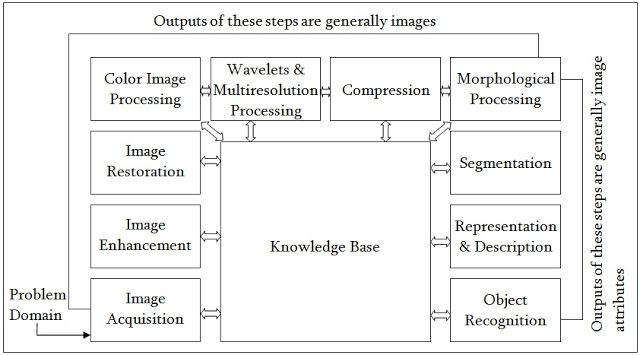
\includegraphics[width=0.6\linewidth]{img/IP.jpg}
            \caption{Fundamental steps in digital processing}
        \end{figure}
        \subsubsection{Image Acquistion}
            This is the first step or process of the fundamental steps of digital image processing. Image acquisition could 
            be as simple as being given an image that is already in digital form. Generally, the image acquisition stage involves 
            preprocessing, such as scaling etc.
        \subsubsection{Image Enhancement}
            Image enhancement is among the simplest and most appealing areas of digital image processing. Basically, the idea behind 
            enhancement techniques is to bring out detail that is obscured, or simply to highlight certain features of interest in an 
            image. Such as, changing brightness \& contrast etc.
        \subsubsection{Image Restoration}
            Image restoration is an area that also deals with improving the appearance of an image. However, unlike enhancement, 
            which is subjective, image restoration is objective, in the sense that restoration techniques tend to be based on mathematical 
            or probabilistic models of image degradation.
        \subsubsection{Color Image Processing}
            Color image processing is an area that has been gaining its importance because of the significant increase in the use of digital 
            images over the Internet. This may include color modeling and processing in a digital domain etc.
        \subsubsection{Wavelets and Multiresolution Processing}
            Wavelets are the foundation for representing images in various degrees of resolution. Images subdivision successively into smaller 
            regions for data compression and for pyramidal representation.
        \subsubsection{Compression}
            Compression deals with techniques for reducing the storage required to save an image or the bandwidth to transmit it. Particularly in 
            the uses of internet it is very much necessary to compress data.
        \subsubsection{Morphological Processing}
            Morphological processing deals with tools for extracting image components that are useful in the representation and description of shape.
        \subsubsection{Segmentation}
            Segmentation procedures partition an image into its constituent parts or objects. In general, autonomous segmentation is one of the most difficult 
            tasks in digital image processing. A rugged segmentation procedure brings the process a long way toward successful solution of imaging problems that 
            require objects to be identified individually.
        \subsubsection{Representation and Description}
            Representation and description almost always follow the output of a segmentation stage, which usually is raw pixel data, constituting either the boundary 
            of a region or all the points in the region itself. Choosing a representation is only part of the solution for transforming raw data into a form suitable 
            for subsequent computer processing. Description deals with extracting attributes that result in some quantitative information of interest or are basic for 
            differentiating one class of objects from another.
        \subsubsection{Object Recognition}
            Recognition is the process that assigns a label, such as, “vehicle” to an object based on its descriptors.
        \subsubsection{Knowledge Base}
            Knowledge may be as simple as detailing regions of an image where the information of interest is known to be located, thus limiting the search that has to be 
            conducted in seeking that information. The knowledge base also can be quite complex, such as an interrelated list of all major possible defects in a materials 
            inspection problem or an image database containing high-resolution satellite images of a region in connection with change-detection applications.
    \subsection{The Components of Image Processing}
        \subsubsection{Digital Image}
            A digital image is a finite set of pixels with a gray level suitable for describing an image close to the real image. The number of pixels 
            determines the resolution of the image. The higher quality of the image, the more clearly the image's points are displayed, making the image 
            more realistic and sharp.
        \subsubsection{Picture Element}
            In digital imaging, pixel, pel, or picture element is a smallest addressable element in a raster image, or the smallest addressable element in an \textbf{all points 
            addressable display device}; so it is the smallest controllable element of a picture represented on the screen. \\ 
            \vspace{3mm}
            Each pixel is a sample of an original image; more samples typically provide more accurate representations of the original. The intensity of each pixel is variable. 
            In color imaging systems, a color is typically represented by three or four component intensities such as red, green, and blue, or cyan, magenta, yellow, and black. \\ 
            \vspace{3mm}
            In some contexts (such as descriptions of \textbf{camera sensors}), pixel refers to a single scalar element of a multi-component representation (called a photosite in the 
            camera sensor context, although sensel is sometimes used), while in yet other contexts it may refer to the set of component intensities for a spatial position.
            \begin{figure}[H]
                \centering
                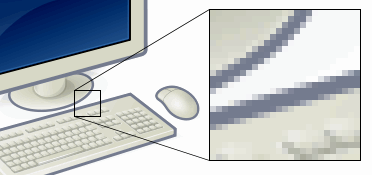
\includegraphics[width=0.6\linewidth]{img/Pixel-example.png}
                \caption{Pixel example}
            \end{figure}
            Pixel is an element of digital image at coordinate (x,y) with gray level or certain color. The size and the distance between those pixels are chosen appropriately so that 
            the human eye perceives spatial continuity and gray level (or color) of digital image like real image. Each of element in matrix is called an image element.
        \subsubsection{Gray Level of Picture}
            Gray level is the result of conversion of 1 luminosity value of 1 pixel positive integer value. Usually identified in [0,255] depending on the value each pixel is 
            represented. Common gray scale values is: 16, 32, 64, 128, 256 (level 256 is universal level). The reason is computer techniques use 1 byte (8 bits) to represent 
            the gray level. Gray level use 1 byte represent: 28 = level 256, it mean from 0 to 255).
            \begin{figure}[H]
                \centering
                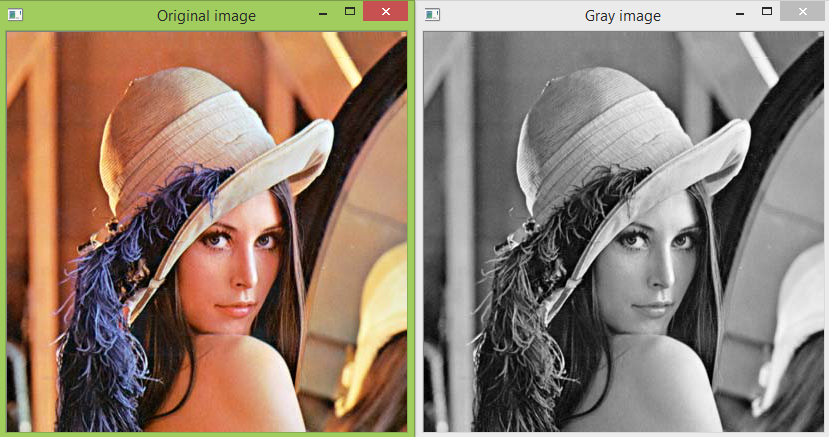
\includegraphics[width=0.6\linewidth]{img/gray-scale.png}
                \caption{Gray scale image example}
            \end{figure}
        \subsubsection{Image Resolution}
            Image resolution is detail an image holds. The term applies to raster digital images, film images, and other types of images. Higher resolution means more image detail. \\ 
            \vspace{3mm}
            Image resolution can be measured in various ways. Resolution quantifies how close lines can be to each other and still be visibly resolved. Resolution units can be tied 
            to physical sizes (e.g. lines per mm, lines per inch), to the overall size of a picture (lines per picture height, also knnown simply as lines, TV lines, or TVL), 
            or to angular subtense. Line pairs are often used instead of lines; a line pair comprises a dark line and an adjacent light line. A line is either a dark line or 
            a light line. A resolution of 10 lines per milimeter means 5 dark line alternating with 5 light lines, or 5 line pairs per milimeter (5 LP/mm). Photographic lens and film 
            resolution are most often quoted in line pairs per milimeter. \\ 
            \vspace{3mm}
            For example: Image resolution in CGA display (Color Graphic Adaptor) is a grid of points across the screen: 320 vertical points * 200 image points (320*200).
            Obviously, with the same CGA display 12 inches we notice smoother than the screen CGA 17 inches with resolution is 320*200. The reason is with the same resolution but 
            the larger the screen area, the less smooth.
        \subsubsection{Types of image classification}
            \begin{itemize}
                \item \textbf{Binary Image:} is one that consists of pixels that can have one of exactly two colors, usually black and white. Binary images are also called bi-level 
                or two-level, Pixelart made of two colours is often referred to as 1-Bit or 1bit. This means that each pixel is stored as a single bit—i.e., a 0 or 1. \\
                \vspace{2mm}
                The names black-and-white, B\&W, monochrome or monochromatic are often used for this concept, but may also designate any images that have only one sample per pixel, 
                such as grayscale images. In Photoshop parlance, a binary image is the same as an image in "Bitmap" mode. \\ 
                \vspace{2mm}
                Binary images often arise in digital image processing as masks or thresholding, and dithering. Some input/output devices, such as laser printers, fax machines, 
                and bilevel computer displays, can only handle bilevel images. \\ 
                \vspace{2mm}
                A binary image can be stored in memory as a bitmap, a packed array of bits. A 640×480 image requires 37.5 KiB of storage. Because of the small size of the image files, 
                fax machine and document management solutions usually use this format. Most binary images also compress well with simple run-length compression schemes. \\ 
                \vspace{2mm}
                Binary images can be interpreted as subsets of the two-dimensional integer lattice $Z^2$; the field of morphological image processing was largely inspired by this view.
                \item \textbf{RGB Image:} RGB Color Model is an additive color model, in which red, green, and blue light are added together in various ways to reproduce a broad array 
                of colors. The name of the model comes from the initials of the three additive primary colors, red, green, and blue. \\ 
                \vspace{2mm}
                RGB is a device-dependent color model: different devices detect or reproduce a given RGB value differently, since the color elements (such as phosphors or dyes) 
                and their response to the individual R, G, and B levels vary from manufacturer to manufacturer, or even in the same device over time. Thus an RGB value does not define 
                the same color across devices without some kind of color management.
                \begin{figure}[H]
                    \centering
                    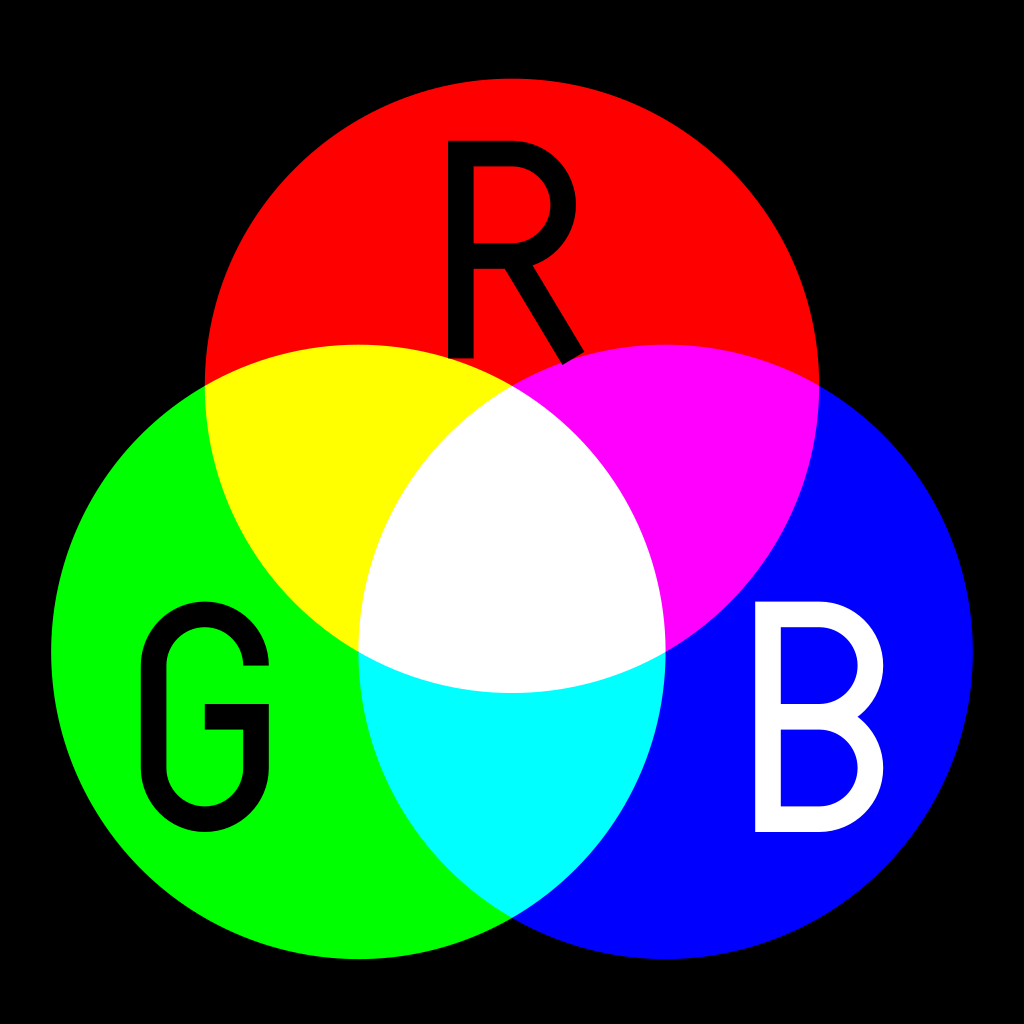
\includegraphics[width=0.6\linewidth]{img/RGB.png}
                    \caption{Additive color mixing}
                \end{figure}
                The choice of primary colors is related to the physiology of the human eye; good primaries are stimuli that maximize the difference between the responses of the cone 
                cells of the human retina to light of different wavelengths, and that thereby make a large color triangle. \\ 
                \vspace{2mm}
                The normal three kinds of light-sensitive photoreceptor cells in the human eye (cone cells) respond most to yellow (long wavelength or L), green (medium or M), 
                and violet (short or S) light (peak wavelengths near 570 nm, 540 nm and 440 nm, respectively). The difference in the signals received from the three kinds allows 
                the brain to differentiate a wide gamut of different colors, while being most sensitive (overall) to yellowish-green light and to differences between hues in the 
                green-to-orange region.
                \begin{figure}[H]
                    \centering
                    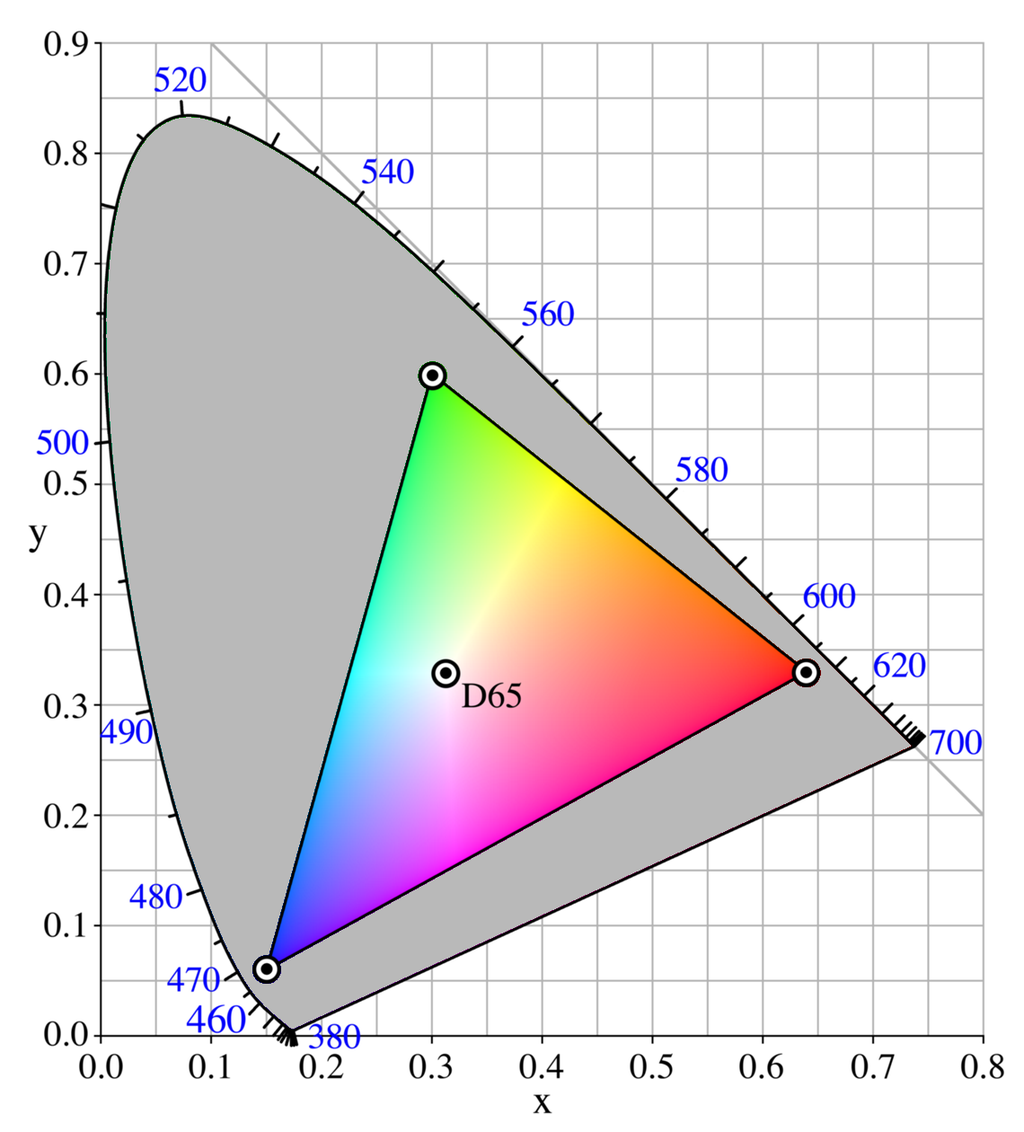
\includegraphics[width=0.6\linewidth]{img/primary-color.png}
                    \caption{A set of primary colors, such as the sRGB primaries, define a color triangle}
                \end{figure}
                \item \textbf{Image Transformation:} is a function. A function that maps one set to another set after performing some operations. \\ 
                \vspace{2mm}
                Image transformation is consider this equation:
                \begin{align}
                    G(x,y) = T{f(x,y)}
                \end{align}
                In this equation, $F(x,y)$ is input image on which transformation function has to be applied; $G(x,y)$ is the output image or processed image; $T$ is the transformation 
                function. This relation between input image and the processed output image can also be represented as: $s = T(r)$ where $r$ is actually the pixel value or gray level intensity 
                of $f(x,y)$ at any point. And $s$ is the pixel value or gray level intensity of $g(x,y)$ at any point. \\
                \vspace{2mm}
                The basic gray level transformation has been discussed in our tutorial of basic gray level transformations. There is some image transformations like: \texttt{Fourier Transform, Cousin, 
                Sin, convolution transform, Kronecker product}.
            \end{itemize}
    \subsection{Parts of The Image Processing System}
        \begin{figure}[H]
            \centering
            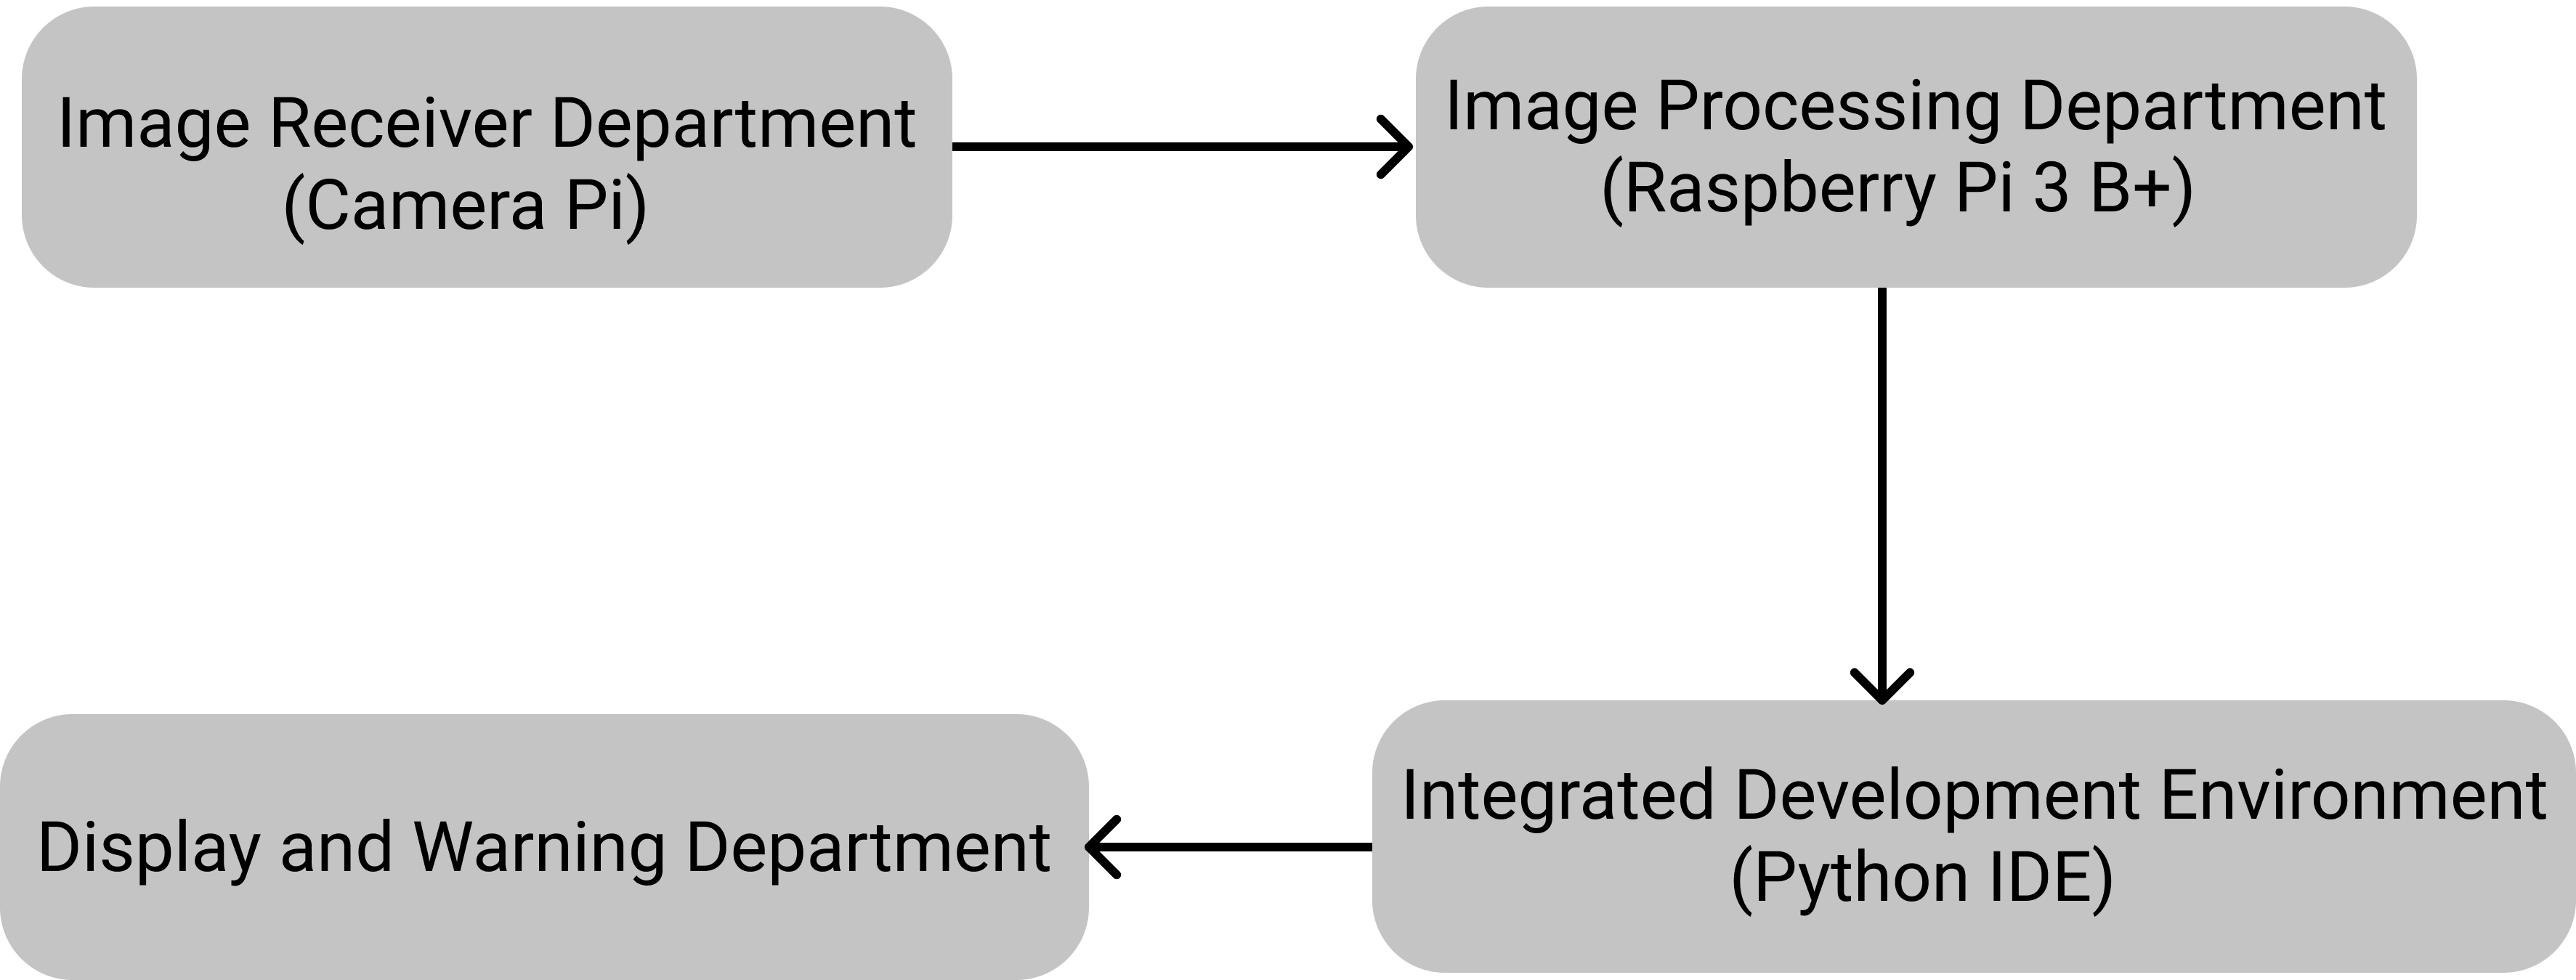
\includegraphics[width=0.6\linewidth]{img/Drowsiness.png}
            \caption{The part of image processing system}
        \end{figure}
        \textbf{Image Receiver Department} is usually a camera, scaners, image sensor,... In this project, a pi camera with 5mpx resolution is used to capture images. \\ 
        \vspace{3mm}
        \textbf{Image Processing Department} is specialized processing equipment or computers,... Specifically here using a Raspberry pi 3B + computer for image processing. \\ 
        \vspace{3mm}
        \textbf{Integrated Development Environment} using Thony Python IDE software to write program. \\ 
        \vspace{3mm}
        \textbf{Warning Devices} speaker alarms.

\section{Face Regconition Algorithm}
    Before we go to the algorithms for face detection we should understand how to detect a face even though we don't know who the subject is. \\
    \vspace{3mm}
    Face Recognition is a way of recognizing a human face through technology. A facial recognition system uses biometrics to map facial features from a photograph or video. 
    It compares the information with a database of known faces to find a match. Facial recognition can help verify personal identity, but it also raises privacy issues. \\ 
    \vspace{3mm}
    The recognition of a face in a video sequence is split into three primary tasks: Face Detection, Face Prediction, and Face Tracking. The tasks performed in the Face Capture 
    program are performed during face recognition as well. To recognize the face obtained, a vector of HOG features of the face is extracted. This vector is then used in the SVM 
    model to determine a matching score for the input vector with each of the labels. The SVM returns the label with the maximum score, which represents the confidence to the 
    closest match within the trained face data. 
    \begin{figure}[H]
        \centering
        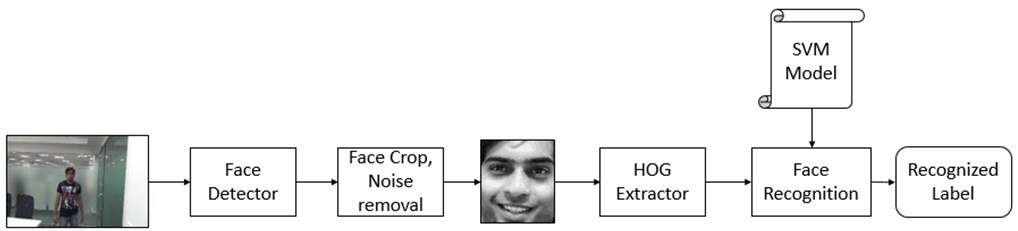
\includegraphics[width=0.6\linewidth]{img/face-recognition.jpg}
        \caption{Block diagram of the face recognition process}
    \end{figure}
    The task of calculating matching scores is exceptionally heavy to compute. Hence, once detected and identified, the labeled face in an image needs to be tracked to reduce the 
    computation in future frames until the face eventually disappears from the video. Of all the available trackers, the Camshift tracking algorithm is used since it produces the 
    best results with faces. \\ 
    \vspace{3mm}
    Where you see a face, recognition technology sees data. That data can be stored and accessed. 
    For instance, half of all American adults have their images stored in one or more facial-recognition databases that law enforcement agencies can search, according to a 
    Georgetown University study. Technologies can be different, but there are the basic steps:
    \begin{itemize}
        \item \textbf{Step 1.} A picture of your face is captured from a photo or video. Your face might appear alone or in a crowd. Your image may show you looking straight 
        ahead or nearly in profile
        \item \textbf{Step 2.} Facial recognition software reads the geometry of your face. Key factors include the distance between your eyes and the distance from forehead to chin. 
        The software identifies facial landmarks — one system identifies 68 of them — that are key to distinguishing your face. The result: your facial signature
        \item \textbf{Step 3.} Your facial signature — a mathematical formula — is compared to a database of known faces. And consider this: at least 117 million Americans have images 
        of their faces in one or more police databases. According to a May 2018 report, the FBI has had access to 412 million facial images for searches
        \item \textbf{Step 4.} A determination is made. Your faceprint may match that of an image in a facial recognition system database.
    \end{itemize}
    The gist of the pipeline can be seen in figure down here: 
    \begin{figure}[H]
        \centering
        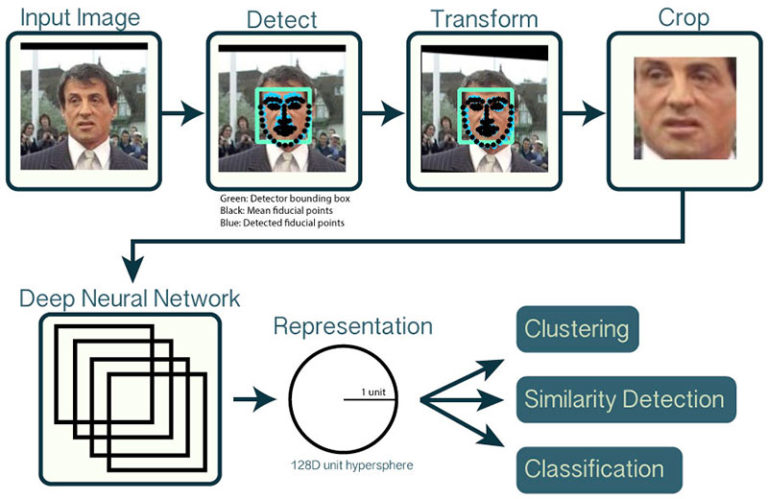
\includegraphics[width=0.6\linewidth]{img/opencv.jpg}
        \caption{An overview of the OpenCV face recognition pipeline}
    \end{figure}
    First, we input an image or video frame to our face recognition pipeline. Given the input image, we apply face detection to detect the location of a face in the image. Optionally 
    we can compute \textbf{Facial Landmarks}, enabling us to \textbf{Preprocess and align the face}. \\ 
    \vspace{3mm}
    Face alignment, as the name suggests, is the process of identifying the geometric structure of the faces and attempting to obtain a canonical alignment of the face based on translation, 
    rotation, and scale. While optional, face alignment has been demonstrated to increase face recognition accuracy in some pipelines. After we’ve (optionally) applied face alignment 
    and cropping, we pass the input face through our deep neural network:
    \begin{figure}[H]
        \centering
        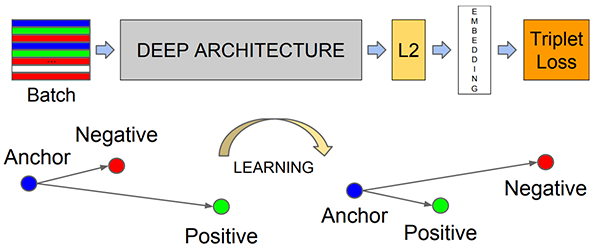
\includegraphics[width=0.6\linewidth]{img/pyimgsearch.png}
        \caption{How the deep learning face recognition model computes the face embedding}
    \end{figure}
    The FaceNet deep learning model computes a 128-d embedding that quantifies the face itself. But how does the network actually compute the face embedding? The answer lies in the training 
    process itself, including:
    \begin{itemize}
        \item The input data to the network
        \item The triplet loss function
    \end{itemize}
    To train a face recognition model with deep learning, each input batch of data includes three images:
    \begin{itemize}
        \item The anchor
        \item The positive image
        \item The negative image
    \end{itemize}
    The anchor is our current face and has identity A. \\ 
    \vspace{3mm}
    The second image is our positive image — this image also contains a face of person A. \\ 
    \vspace{3mm}
    The negative image, on the other hand, does not have the same identity, and could belong to person B, C, or even Y! \\
    \vspace{3mm}
    The point is that the anchor and positive image both belong to the same person/face while the negative image does not contain the same face. The neural network computes the 128-d 
    embeddings for each face and then tweaks the weights of the network (via the triplet loss function) such that:
    \begin{itemize}
        \item The 128-d embeddings of the anchor and positive image lie closer together
        \item While at the same time, pushing the embeddings for the negative image father away
    \end{itemize}
    In this manner, the network is able to learn to quantify faces and return highly robust and discriminating embeddings suitable for face recognition.
    \subsection{Face Detection using HOG}
        The essential thought behind the histogram of oriented gradients descriptor is that local object appearance and shape within an image can be described by the distribution of intensity gradients or edge directions. 
        The image is divided into small connected regions called cells, and for the pixels within each cell, a histogram of gradient directions is compiled. The descriptor is the concatenation of these histograms. For 
        improved accuracy, the local histograms can be contrast-normalized by calculating a measure of the intensity across a larger region of the image, called a block, and then using this value to normalize all cells 
        within the block. This normalization results in better invariance to changes in illumination and shadowing. \\
        \vspace{3mm}
        In the current example, all the face sample images of a person are fed to the feature descriptor extraction algorithm; i.e., a HOG. The descriptors are gradient vectors generated per pixel of the image. 
        The gradient for each pixel consists of magnitude and direction, calculated using the following formular:
        \begin{figure}[H]
            \centering
            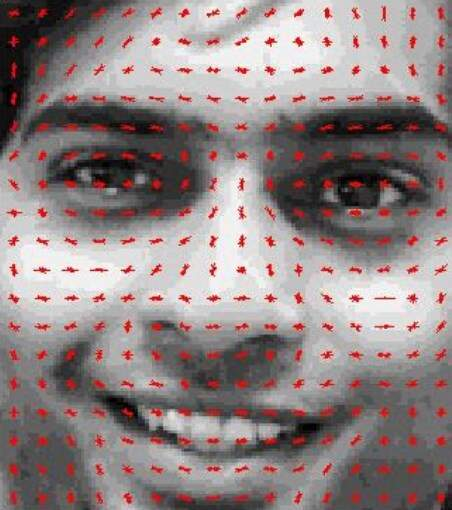
\includegraphics[width=0.6\linewidth]{img/HOG-feature.jpg}
            \caption{HOG features sample face}
        \end{figure}
        \begin{align}
            g = \sqrt{g^2_x + g^2_y} \\ 
            \theta = \arctan{\frac{g_y}{g_x}}
        \end{align}
        Gx and Gy are respectively the horizontal and vertical components of the change in the pixel intensity. A window size of 128 x 144 is used for face images since it matches the general aspect ratio of human faces. 
        The descriptors are calculated over blocks of pixels with 8 x 8 dimensions. These descriptor values for each pixel over 8 x 8 block are quantized into 9 bins, where each bin represents a directional angle of gradient 
        and value in that bin, which is the summation of the magnitudes of all pixels with the same angle. \\ 
        \vspace{3mm}
        Further, the histogram is then normalized over a 16 x 16 block size, which means four blocks of 8 x 8 are normalized together to minimize light conditions. This mechanism mitigates the accuracy drop due to a 
        change in light. The SVM model is trained using a number of HOG vectors for multiple faces. \\
        \vspace{3mm}
        There is some review entire detailed process of training an object detector using Histogram Oriented Gradients, each step can be fairly detailed. It goes like something like this:
        \begin{itemize}
            \item \textbf{Step 1:} Sample P positive samples from your training data of the object(s) you want to detect and extract HOG descriptors from these samples;
            \item \textbf{Step 2:} Sample N negative samples from a negative training set that \textbf{does not contain} any of the objects you want to detect and extract HOG descriptors from these samples as well. In practice N $\gg$ P;
            \item \textbf{Step 3:} Train a Linear Support Vector Machine on your positive and negative samples;
            \item \textbf{Step 4:} 
                \begin{figure}[H]
                    \centering
                    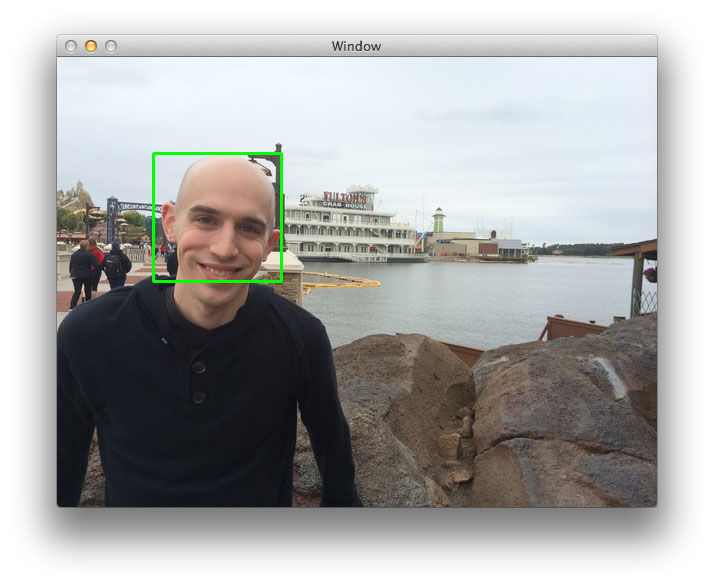
\includegraphics[width=0.6\linewidth]{img/sliding_window_example.jpg}
                    \caption{Example of the sliding a window approach, where we slide a window from left-to-right and top-to-bottom}
                \end{figure}
                \textbf{Apply hard-negative mining}, For each image and each possible scale of each image in your negative training set, apply the sliding window technique and slide your window across the image. 
                At each window compute your HOG descriptors and apply your classifier. If your classifier (incorrectly) classifies a given window as an object (and it will, there will absolutely be false-positives), 
                record the feature vector associated with the false-positive patch along with the probability of the classification. \textbf{This approach is called hard-negative mining}.
            \item \textbf{Step 5:} Take the false-positive samples found during the hard-negative mining stage, sort them by their confidence (i.e. probability) and re-train your classifier using these hard-negative samples.
            \item \textbf{Step 6:} Your classifier is now trained and can be applied to your test dataset. Again, just like in Step 4, for each image in your test set, and for each scale of the image, apply the sliding window technique. 
                At each window extract HOG descriptors and apply your classifier. If your classifier detects an object with sufficiently large probability, record the bounding box of the window. After you have finished scanning the image, 
                apply non-maximum suppression to remove redundant and overlapping bounding boxes. \\ 
                \vspace{2mm}
                These are the bare minimum steps required, but by using this 6-step process you can train and build object detection classifiers of your own! Extensions to this approach include a deformable parts model and Exemplar SVMs, 
                where you train a classifier for each positive instance rather than a collection of them. \\ 
                \vspace{2mm}
                However, if you’ve ever worked with object detection in images you’ve likely ran into the problem of detecting multiple bounding boxes around the object you want to detect in the image. And here’s an example of this overlapping bounding box problem:
                \begin{figure}[H]
                    \centering
                    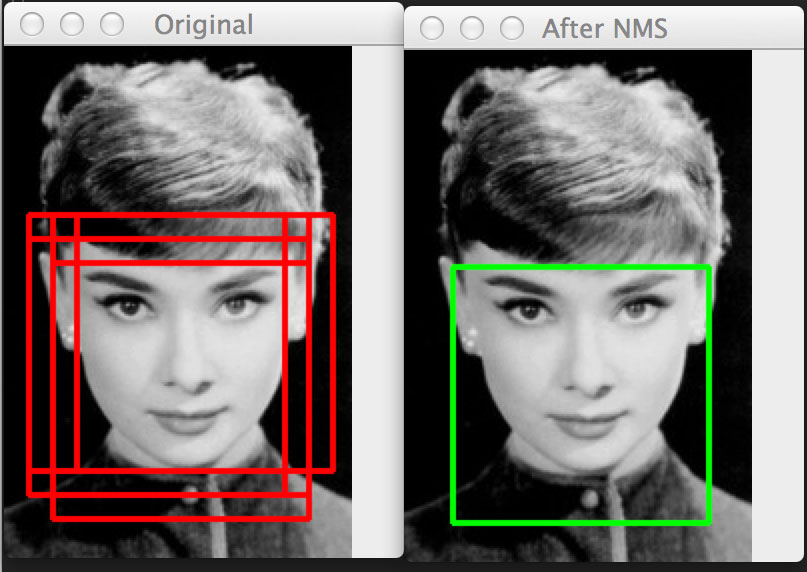
\includegraphics[width=0.6\linewidth]{img/multiple-overlapping.jpg}
                    \caption{(Left) Detecting multiple overlapping bounding boxes around the face we want to detect. (Right) Applying non-maximum suppression to remove the redundant bounding boxes.}
                \end{figure}
        \end{itemize}
    \subsection{Haar-like Feature (Haar-Cascade)}
        \subsubsection{Theory}
            Object Detection using Haar feature-based cascade classifiers is an effective object detection method is a machine learning based approach where a cascade function is trained from a lot of positive and negative images. It is then used to detect objects in other images. \\ 
            \vspace{3mm}
            Here we will work with face detection. Initially, the algorithm needs a lot of positive images (images of faces) and negative images (images without faces) to train the classifier. Then we need to extract features from it. For this, Haar features shown in the below image 
            are used. They are just like our convolutional kernel. Each feature is a single value obtained by subtracting sum of pixels under the white rectangle from sum of pixels under the black rectangle.
            \begin{figure}[H]
                \centering
                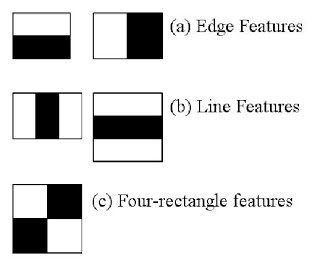
\includegraphics[width=0.6\linewidth]{img/haar_features.jpg}
                \caption{Feature 4 rectangle}
            \end{figure}
            \begin{figure}[H]
                \centering
                
\includegraphics[width=0.6\linewidth]{img/feature_center.png}
                \caption{Feature in center}
            \end{figure}
            Using above features, we can calculate the value of the Haar-Like feature as the difference between the sum of the pixels of the black area and the white area as shown in the following formula:
            \begin{align}
                F(x) = Sum of black area - Sum of white area (gray level of pixel)
            \end{align} 
            There is a concept called \textbf{"Integral Image"}, is the 2D array with the size equal to the size of the image to be Haar-Like feature, with each element of this array is computed by summing the pixels above and left of it.
        \subsubsection{Integral Image}
            The idea of this concept is transforming an input images into a summed-area table, where the value at any point (x, y) in that table is the sum of all the pixels above and to the left of (x, y), inclusive:
            \begin{align}
                P(x,y) = \Sigma_{x' \leq x, y' \leq y} i(x',y')
            \end{align}
            Where I(x,y) is the value of the integral image pixel in the position (x,y), while i(x,y) is the corresponding intensity in the original image. It is a recursive formula, hence, if we start from one corner of the input image, we will have the same result in the integral image. 
            To make it clearer, let’s see an example:
            \begin{figure}[H]
                \centering
                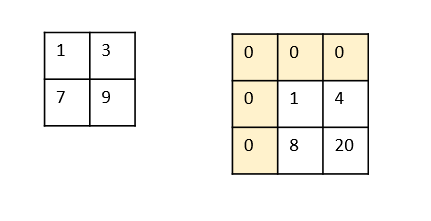
\includegraphics[width=0.6\linewidth]{img/example_integral.png}
                \caption{Example of Integral Image}
            \end{figure}
            In this figure we added one row and column of zeros, since we need one step backward in order to start the recursive formula. Hence, if your image is $w$ pixels wide and $h$ pixels high, then the integral of this will be $w+1$ pixels wide and $h+1$ pixels high. \\ 
            \vspace{3mm}
            Moving to the computations, let's start from the first pixel in the original image with intensity 1: the integral image returns exactly the same value, since it is computing (1+0+0). Then, pixel '3' becomes '4', since it is 3+1+0+0. With the same procedure, we obtain an 
            "8" (7+1+0) and a '20' (9+3+1+7). \\ 
            \vspace{3mm}
            We have a new image, but how is supposed to be useful? The answer rely in an unique property of the integral image. Indeed, it turned our that if you need to compute the summation within a window in the input image, hence that summation is equal to a linear combination 
            of the corresponding window’s corner in the integral image, as follows:
            \begin{align}
                \Sigma_{x_0 < x < x_1; y_0 < y < y_1} i(x,y) = I(D) + I(A) - I(B) - I(C)
            \end{align}
            Where is $A,B,C$ and $D$ are the corners of the corresponding window in the integral image.
            \begin{figure}[H]
                \centering
                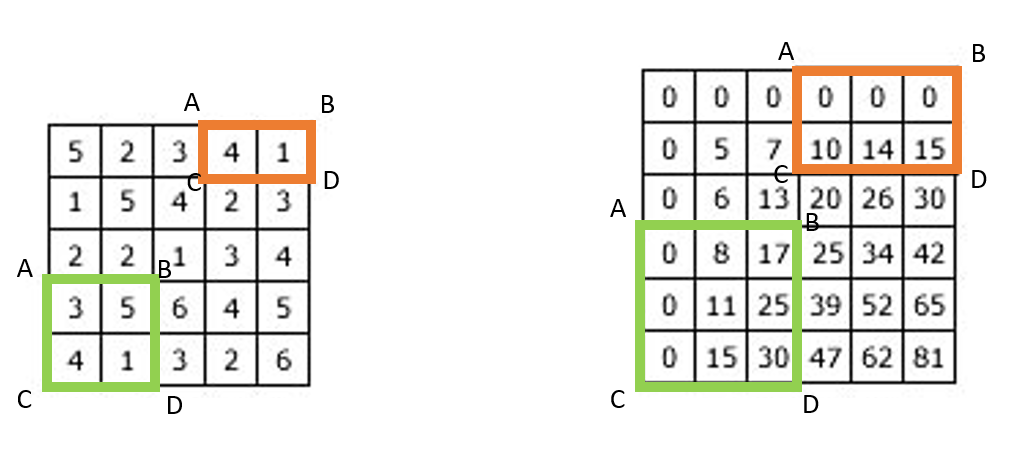
\includegraphics[width=0.6\linewidth]{img/corners_corresponding.png}
                \caption{Integral Image Approach}
            \end{figure}
            This reduces the number of computations by far. To give you an idea, consider a 100×100 image with a 9×9 window. We want to compute the sum of the pixel intensities within that window, which requires 8 operations. If we repeat this procedure 100 times, we obtain 800 operations. \\
            \vspace{3mm}
            Now let’s see the integral image approach. First, we compute the summed-area table, which requires 56 operations. Then, considering the same 9×9 window, to compute the sum of pixel intensity we just need the above formula, which is made of 3 operations. Hence, the total number 
            of operations is 56+3*100=356. As you can see, it is less than a half. \\
            \vspace{3mm}
            This procedure is widely used in computer vision and Haar Cascade algorithm is based exactly on that. \\
            \vspace{3mm}
            Now, all possible sizes and locations of each kernel are used to calculate lots of features. (Just imagine how much computation it needs? Even a 24x24 window results over 160000 features). For each feature calculation, we need to find the sum of the pixels under white 
            and black rectangles. To solve this, they introduced the integral image. However large your image, it reduces the calculations for a given pixel to an operation involving just four pixels. It makes things super-fast. \\ 
            \vspace{3mm}
            But among all these features we calculated, most of them are irrelevant. For example, consider the image below. The top row shows two good features. The first feature selected seems to focus on the property that the region of the eyes is often darker than the region of 
            the nose and cheeks. The second feature selected relies on the property that the eyes are darker than the bridge of the nose. But the same windows applied to cheeks or any other place is irrelevant. So how do we select the best features out of 160000+ features? 
            It is achieved by \textbf{Adaboost}.
            \begin{figure}[H]
                \centering
                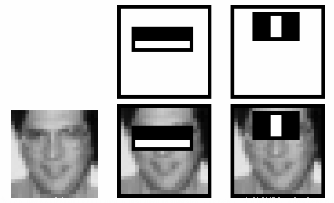
\includegraphics[width=0.6\linewidth]{img/haar_example.png}
                \caption{Example for this feature}
            \end{figure}
            For this, we apply each and every feature on all the training images. For each feature, it finds the best threshold which will classify the faces to positive and negative. Obviously, there will be errors or misclassifications. We select the features with minimum error rate, 
            which means they are the features that most accurately classify the face and non-face images. (The process is not as simple as this. Each image is given an equal weight in the beginning. After each classification, weights of misclassified images are increased. Then the same 
            process is done. New error rates are calculated. Also new weights. The process is continued until the required accuracy or error rate is achieved or the required number of features are found). \\ 
            \vspace{3mm}
            The final classifier is a weighted sum of these weak classifiers. It is called weak because it alone can't classify the image, but together with others forms a strong classifier. The paper says even 200 features provide detection with 95\% accuracy. Their final setup had 
            around 6000 features. (Imagine a reduction from 160000+ features to 6000 features. That is a big gain). \\ 
            \vspace{3mm}
            So now take an image. Take each 24x24 window. Apply 6000 features to it. Check if it is face or not. There will be a little inefficient and time consuming. There is a good solution for that. \\ 
            \vspace{3mm}
            In an image, most of the image is non-face region. So it is a better idea to have a simple method to check if a window is not a face region. If it is not, discard it in a single shot, and don't process it again. Instead, focus on regions where there can be a face. This way, 
            we spend more time checking possible face regions. \\ 
            \vspace{3mm}
            For this they introduced the concept of Cascade of Classifiers. Instead of applying all 6000 features on a window, the features are grouped into different stages of classifiers and applied one-by-one. Normally the first few stages will contain very many fewer features. 
            If a window fails the first stage, discard it. We don't consider the remaining features on it. If it passes, apply the second stage of features and continue the process. The window which passes all stages is a face region.
    \subsection{AdaBoost Algorithm}
        In recent years, boosting algorithms gained massive popularity in data science or machine learning competitions. Most of the winners of these competitions use boosting algorithms to achieve high accuracy. These Data science competitions provide 
        the global platform for learning, exploring and providing solutions for various business and government problems. Boosting algorithms combine multiple low accuracy(or weak) models to create a high accuracy(or strong) models. It can be utilized in 
        various domains such as credit, insurance, marketing, and sales. Boosting algorithms such as AdaBoost, Gradient Boosting, and XGBoost are widely used machine learning algorithm to win the data science competitions. In this tutorial, you are going 
        to learn the AdaBoost ensemble boosting algorithm, and the following topics will be covered:
        \begin{itemize}
            \item Ensemble Machine Learning Approach
                \begin{itemize}
                    \item Bagging
                    \item Boosting
                    \item Stacking  
                \end{itemize}
            \item Adaboost Classifier
            \item How does the AdaBoost algorithm work?
        \end{itemize}
        \subsubsection{Ensemble Machine Learning Approach}
            An ensemble is a composite model, combines a series of low performing classifiers with the aim of creating an improved classifier. Here, individual classifier vote and final prediction label returned that performs majority voting. Ensembles offer more 
            accuracy than individual or base classifier. Ensemble methods can parallelize by allocating each base learner to different-different machines. Finally, you can say Ensemble learning methods are meta-algorithms that combine several machine learning methods 
            into a single predictive model to increase performance. Ensemble methods can decrease variance using bagging approach, bias using a boosting approach, or improve predictions using stacking approach.
            \begin{figure}[H]
                \centering
                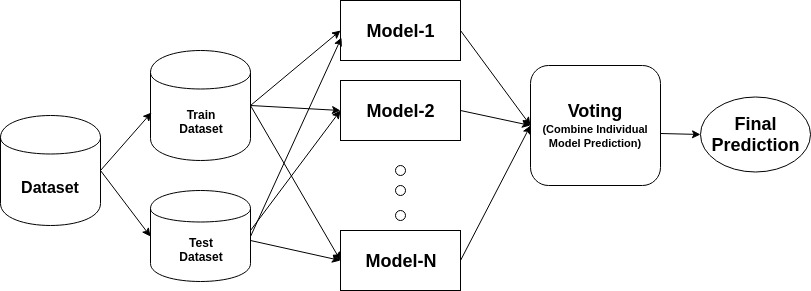
\includegraphics[width=0.6\linewidth]{img/Ensemble.png}
                \caption{Ensemble methods}
            \end{figure}
            \begin{enumerate}
                \item \textbf{Bagging} stands for bootstrap aggregation. It combines multiple learners in a way to reduce the variance of estimates. For example, random forest trains M Decision Tree, you can train M different trees on different random subsets of the 
                data and perform voting for final prediction. Bagging ensembles methods are Random Forest and Extra Trees;
                \item \textbf{Boosting algorithms} are a set of the low accurate classifier to create a highly accurate classifier. Low accuracy classifier (or weak classifier) offers the accuracy better than the flipping of a coin. Highly accurate classifier( or strong classifier) 
                offer error rate close to 0. Boosting algorithm can track the model who failed the accurate prediction. Boosting algorithms are less affected by the overfitting problem. The following three algorithms have gained massive popularity in data science competitions.
                    \begin{itemize}
                        \item AdaBoost (Adaptive Boosting)
                        \item Gradient Tree Boosting
                        \item XGBoost
                    \end{itemize}
                \item \textbf{Stacking (or stacked generalization)} is an ensemble learning technique that combines multiple base classification models predictions into a new data set. This new data are treated as the input data for another classifier. This classifier employed to 
                solve this problem. Stacking is often referred to as blending.
                    \begin{figure}[H]
                        \centering
                        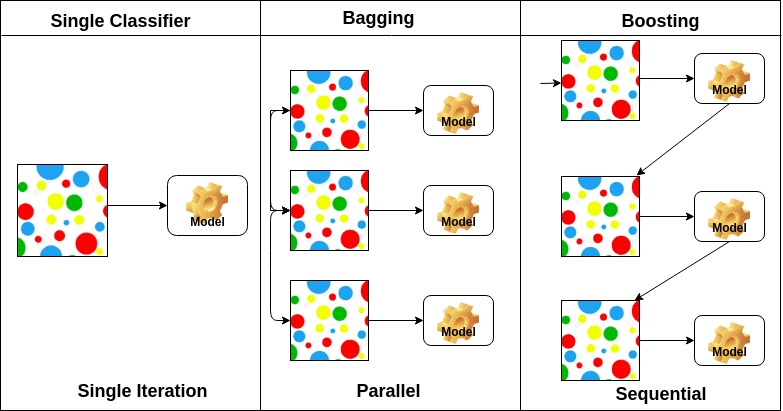
\includegraphics[width=0.6\linewidth]{img/stacking.png}
                        \caption{On the basis of the arrangement of base learners, ensemble methods can be divided into two groups: In parallel ensemble methods, base learners are generated in parallel for example. Random Forest. In sequential ensemble methods, base learners are generated sequentially for example AdaBoost.}
                    \end{figure}
            \end{enumerate}
            On the basis of the type of base learners, ensemble methods can be divided into two groups: homogenous ensemble method uses the same type of base learner in each iteration. heterogeneous ensemble method uses the different type of base learner in each iteration.
        \subsubsection{AdaBoost Classifier}
            Ada-boost or Adaptive Boosting is one of ensemble boosting classifier proposed by Yoav Freund and Robert Schapire in 1996. It combines multiple classifiers to increase the accuracy of classifiers. AdaBoost is an iterative ensemble method. 
            AdaBoost classifier builds a strong classifier by combining multiple poorly performing classifiers so that you will get high accuracy strong classifier. The basic concept behind Adaboost is to set the weights of classifiers and training the 
            data sample in each iteration such that it ensures the accurate predictions of unusual observations. Any machine learning algorithm can be used as base classifier if it accepts weights on the training set. Adaboost should meet two conditions:
            \begin{enumerate}
                \item The classifier should be trained interactively on various weighed training examples;
                \item In each iteration, it tries to provide an excellent fit for these examples by minimizing training error.
            \end{enumerate}
        \subsubsection{How Does AdaBoost Algorithm Work?}
            It works in the following steps:
            \begin{enumerate}
                \item Initially, Adaboost selects a training subset randomly;
                \item It iteratively trains the AdaBoost machine learning model by selecting the training set based on the accurate prediction of the last training;
                \item It assigns the higher weight to wrong classified observations so that in the next iteration these observations will get the high probability for classification;
                \item Also, It assigns the weight to the trained classifier in each iteration according to the accuracy of the classifier. The more accurate classifier will get high weight;
                \item This process iterate until the complete training data fits without any error or until reached to the specified maximum number of estimators;
                \item To classify, perform a "vote" across all of the learning algorithms you built.
            \end{enumerate}
            \begin{figure}[H]
                \centering
                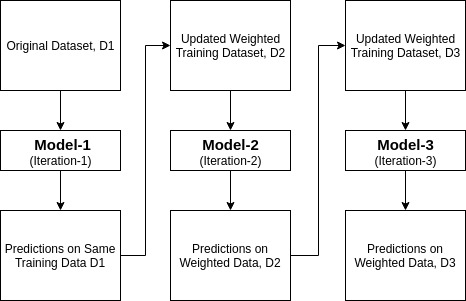
\includegraphics[width=0.6\linewidth]{img/Adaboost work.png}
                \caption{Adaboost model work}
            \end{figure}
            \begin{align}
                h_k = \left\{
                    \begin{array}{ll}
                        1 & \mbox{$p_k f_k(x) < p_k \theta_k$} \\
                        0 & \mbox{opposite}
                    \end{array}
                \right.
            \end{align}
            With: 
            \begin{itemize}
                \item $x$: Subwindow need to consider
                \item $\theta$: threshold
                \item $f_k$: Haar-like characteristic value
                \item $p_k$: Decision coefficient of detemining the dimension of the equation
            \end{itemize}
            Adaboost will combine weak classifiers into strong classifier as follows:
            \begin{align}
                H(x) = \Sigma(a_1 h_1(x) + a_2 h_2(x) +...+ a_n h_n(x))
            \end{align}
            With: $a_t >= 0$ is normalization coefficient for weak classifiers.
            \begin{figure}[H]
                \centering
                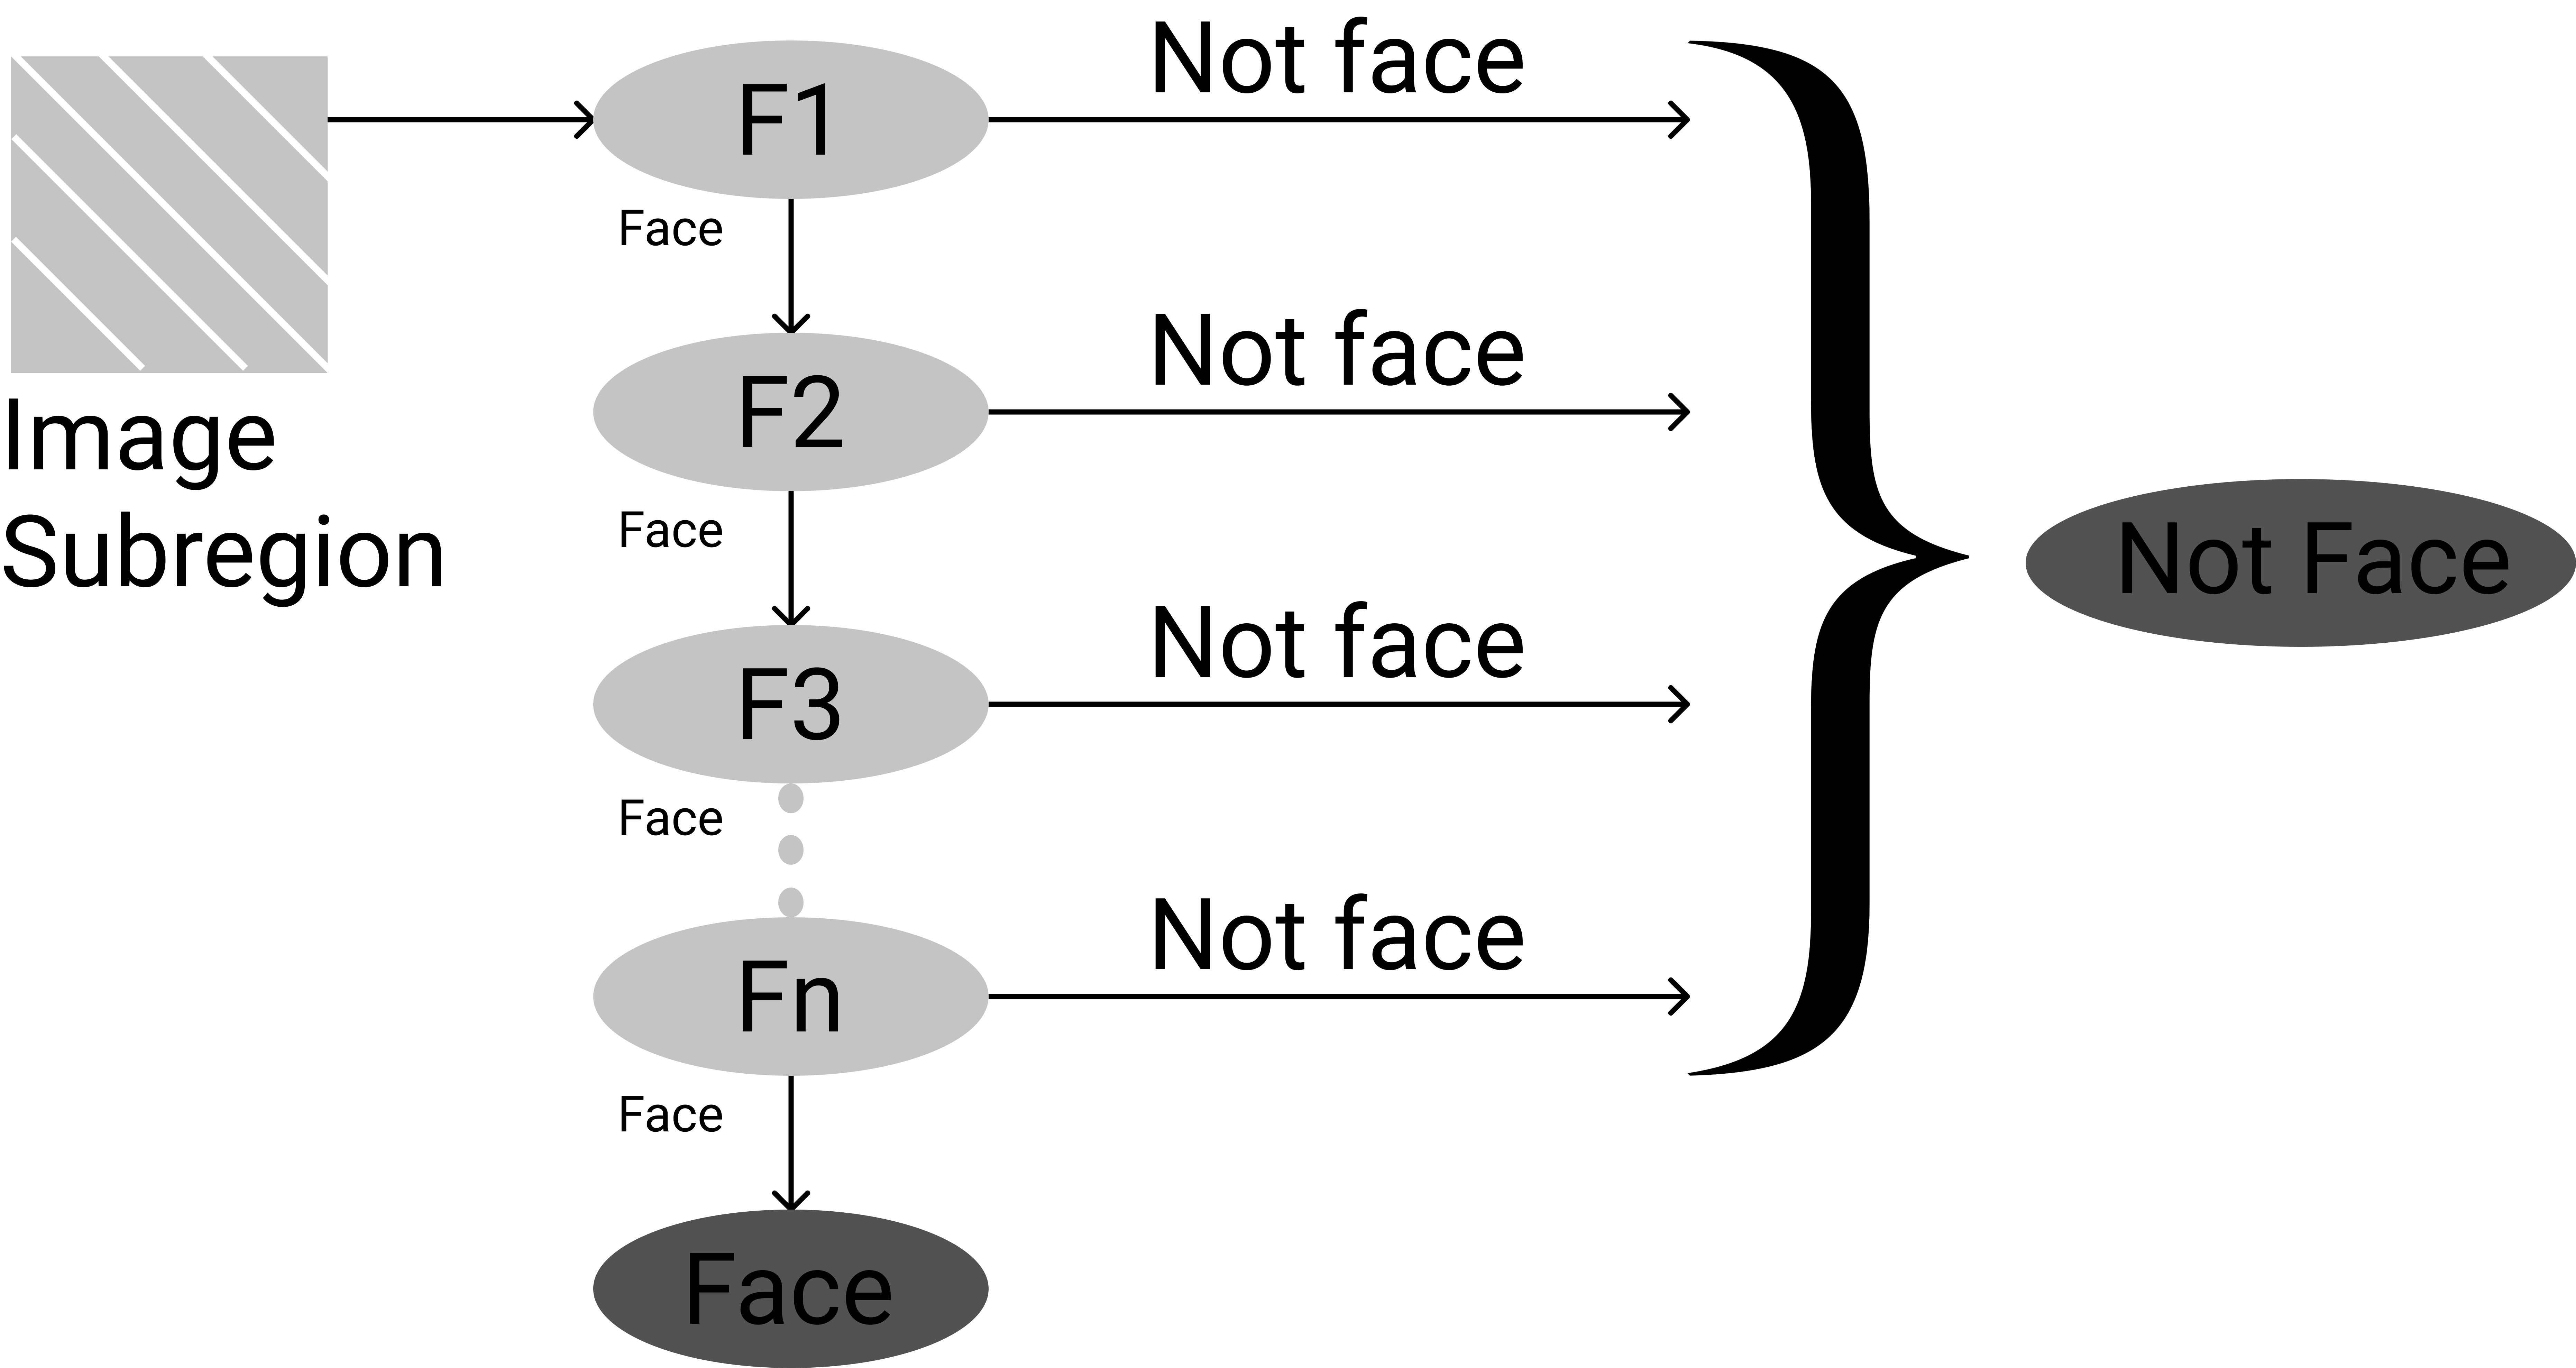
\includegraphics[width=0.6\linewidth]{img/Haar-Cascade.png}
                \caption{Haar Cascade Detection model}
            \end{figure}

\section{Euclidean Distance}

\section{OpenCV}

\section{Python Programming Language}

\section{Introduction about Dlib}

\section{Raspberry Pi 3B +}

    \chapter{MULTIPLE OBJECT TRACKING}

\renewcommand{\headrulewidth}{0.5pt}
\renewcommand{\footrulewidth}{0.5pt}
\thispagestyle{plain}
\pagestyle{fancy}
\fancyhf{}
\fancyhead[L]{\textbf{CHAPTER 3}}
\fancyhead[R]{\textbf{Intelligent Traffic System}}
\raggedright
\fancyfoot[L]{From: ITM Vision}
\fancyfoot[R]{Page \thepage}

\section{Overview}
    Multiple object tracking can be viewed as a multi-variable estimation problem. Given an image sequence, we employ
    $s_t^i$ to denote the state of the i-th object in the t-th frame, $\textbf{S}_t = (s_t^1, s_t^2, ..., s_t^{M_t})$
    to denote states of all the $M_t$ objects in the t-th frame. Let \textbf{$s_{i_s:i_c}^i = \{s_{i_s}^i,...,s_{i_e}^i\}$} 
    be the sequential states of the i-th object, where $i_s$ and $i_e$ are respectively the first and last frame in 
    which target \emph{i} exist, and \textbf{$S_{1:t} = \{S_1,S_2,...,S_t\}$} to denote all the sequential states of all the 
    objects from the first frame to the t-th frame. Note that the object number may vary from frame to frame. \\ 
    \vspace{3mm}
    Correspondingly, following the most commonly used tracking by detection, or Detection Based Tracking (DBT) paradigm,
    we utilize $o_t^i$ to denote the collected observations for the i-th object in the t-th frame. $\textbf{O}_t=(\textbf{o}_t^1,\textbf{o}_t^2,...,\textbf{o}_t^{M_t})$ 
    to denote the collected observations for all the $M_t$ objects in the t-th frame, and $\textbf{O}_{1:t}=\{\textbf{O}_1,\textbf{O}_2,...,\textbf{O}_t\}$ 
    to denote all collected sequential observations of all the objects from the first frame to the t-th frame.
    \vspace{3mm}
    The objective of multiple object tracking is to find the “optimal” sequential states of all the objects, which can be 
    generally modeled by performing MAP (maximal a posteriori) estimation from the conditional distribution of the 
    sequential states given all the observations: 
    \begin{align}
        \hat{S}_{1:t}=\underset{S_{1:t}}{argmax}P(\textbf{S}_{1:t}|\textbf{O}_{1:t})
    \end{align} 
    Different MOT algorithms from previous works can now be thought as designing different approaches to solving 
    the above MAP problem, either from a probabilistic inference perspective or a deterministic optimization perspective. 

\section{Categorization}
    Categorization of MOT bases on: initialization method, processing mode and type of output.
    \begin{itemize}
        \item Initialization method: MOT devides into detection based tracking and detection free tracking
            \begin{itemize}
                \item Detection based tracking: Given a sequence, type specific object detection or motion detection (based on background modeling) is applied in each frame 
                to obtain object hypotheses, then (sequential or batch) tracking is conducted to link detection hypotheses into trajectories. Detection based tracking focuses 
                on specific objects and its performance relies heavily on accuracy of object detectors. Detection based tracking is more popular as it can deal with new 
                discovered and disappear objects automatically.
                \item Detection free tracking requires requires manual initialization of objects in each frame.
                    \begin{figure}[H]
                        \centering
                        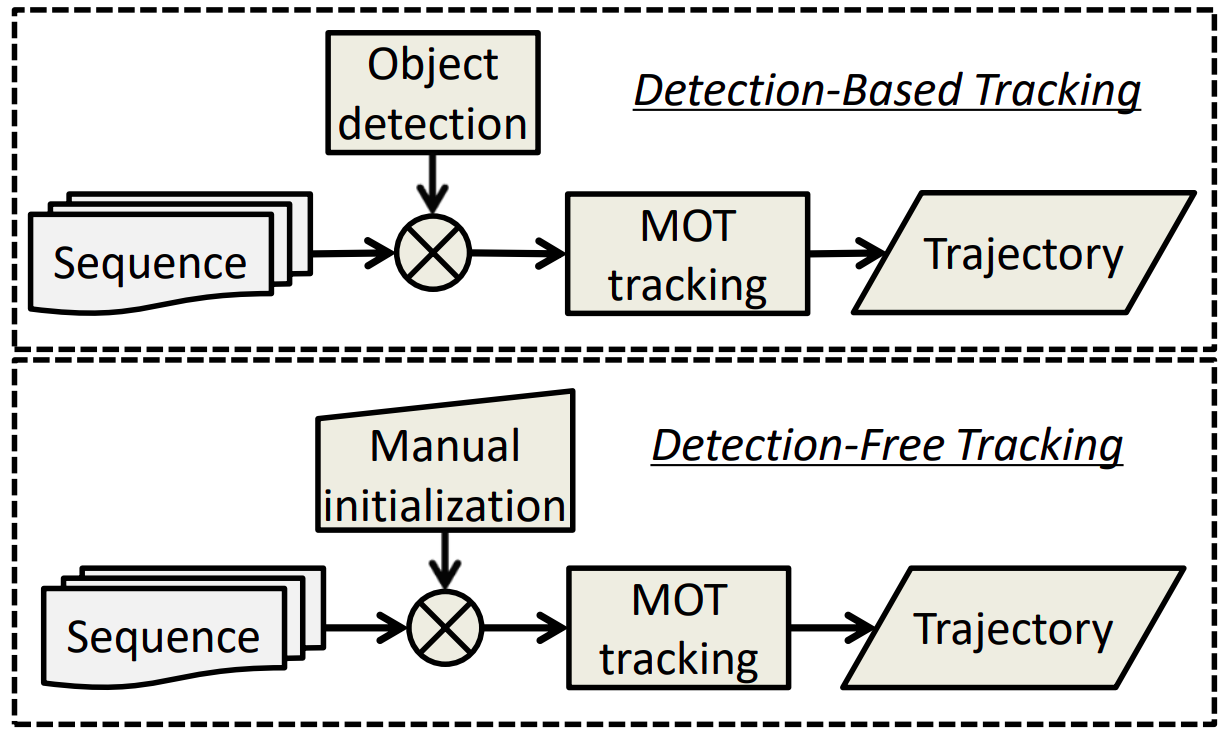
\includegraphics[width=0.6\linewidth]{img/MOT.png}
                        \caption{Pipeline of detection based tracking and detection free tracking}
                    \end{figure}
            \end{itemize}
        \item Processing mode: based on processing mode, MOT can be divided into online tracking and offline tracking problem. 
            \begin{itemize}
                \item An online model receives video input on a frame-by-frame basis, and has to give an output for each frame. This means that, in addition to the current frame, 
                only information from past frames can be used. Online tracking takes up-to-time observation and updates trajectories on the fly there for it is suitable for real time application.
                \item Offline models, on the other hand, have access to the entire video, which means that information from both past and future frames can be used. The task can then be viewed as an 
                optimization problem, where the goal is to find a set of paths that minimize some global loss  function. Offline tracking takes a batch of frames to process therefore it products delay results. 
                Since offline trackers have access to more information, one can expect better performance from these models. 
            \end{itemize}
    \end{itemize}
    Detection free tracking process data sequentially while in Detection based tracking, tracklet or detection response are often associated in batch. \\ 
    \vspace{3mm}
    Recently with the rise of deep learning, MOT can also devided into non-deep learning based methods and deep learning based methods. \\ 
    \vspace{3mm}
    In deep learning based methods, first CNN-based object detectors are applied such as Faster R-CNN and YOLOv3 to localize all objects of interest in input images. Then in a separate step,they crop the images 
    according to the boxes and feed them to an identity embedding network to extract re-ID features which are used to link the boxes over time. The linking step usually follows a standard practice which first 
    computes a cost matrix according to the re-ID features and Intersection over Unions (IoU) of the bounding boxes and then uses the Kalman Filter and Hungarian algorithm to accomplish the linking task. 
    MOT methods based on deep learning can be further devided into two-stage method and one-stage method. \\ 
    \vspace{3mm}
    The main advantage of the two-step methods is that they can develop the most suitable model for each task separately without making compromise. In addition, they can crop the image patches according to the 
    detected bounding boxes and resize them to the same size before estimating re-ID features. This helps to handle the scale variations of objects.The main drawback due to the fact that they are usually very 
    slow because the two tasks need to be done separately without sharing. \\ 
    \vspace{3mm}
    For one stage method, the core idea is to simultaneously accomplish object detection and identity embedding (re-ID features) in a single network in order to reduce inference time. However, the accuracy of the 
    one-shot trackers is usually lower than that of the two-step ones.

\section{MOT Components Overview}
    \subsection{Appearance Model}
        Appearance model includes visual representation and statistical measuring. Appearance model is important cue for affinity computation in MO. Visual representation: local features, region features, 
        Probabilistic Occupancy Map (POM), depth features, Statistical measuring: single cue \& multiple cues (five kinds of fusion strategies: Boosting, Concatenating, Summation, Product, and Cascading).
    \subsection{Motion Model}
        Motion model includes linear \& non-linear model. It aims to estimates the potential position of objects in the future frames, thereby reducing the search space.
    \subsection{Interaction Model} 
        Interaction model, also known as mutual motion model, captures the influence of an object on other objects. In the crowd scenery, an object would experience some “force” from other agents and objects. 
        Interaction model includes social force model \& crowd motion pattern model.
    \subsection{Exclusion Model}
        Exclusion model includes detection-level exclusion \& trajectory-level exclusion. Exclusion is a constraint employed to avoid physical collisions when seeking a solution to the MOT problem. It arises from 
        the fact that two distinct objects cannot occupy the same physical space in the real world.
    \subsection{Occlusion Handling}
        Occlusion is perhaps the most critical challenge in MOT. It is a primary cause for ID switches or fragmentation of trajectories. In order to handle occlusion, various kinds of strategies have been proposed such as: 
        part-to-whole, hypothesize-and-test, buffer-and-recover.
    

\section{Detection Based Tracking and End to End Tracking}

\section{SORT}

\section{Deep SORT}

    \subsection{Feature Extraction and Embedding}

    \subsection{Affinity Computation and Data Association}

\section{Metrics and Evaluations}

    \subsection{Conventional Metrics}

    \subsection{Update Metrics}

    \chapter{INTRODUCTION ABOUT MPIC SYSTEM}

\renewcommand{\headrulewidth}{0.5pt}
\renewcommand{\footrulewidth}{0.5pt}
\thispagestyle{plain}
\pagestyle{fancy}
\fancyhf{}
\fancyhead[L]{\textbf{CHAPTER 4}}
\fancyhead[R]{\textbf{Graduate Report}}
\raggedright
\fancyfoot[L]{From: Nguyen Van Anh Tuan}
\fancyfoot[R]{Page \thepage}

\justifying

\section{Simulation Interface Concept}
    \subsection{What is an interface module?}
        It is the module that allow the software to control and to monitor the cockpit hardware.
    \subsection{MPIC Interface System Overview Software Module}
        \begin{figure}[H]
            \centering
            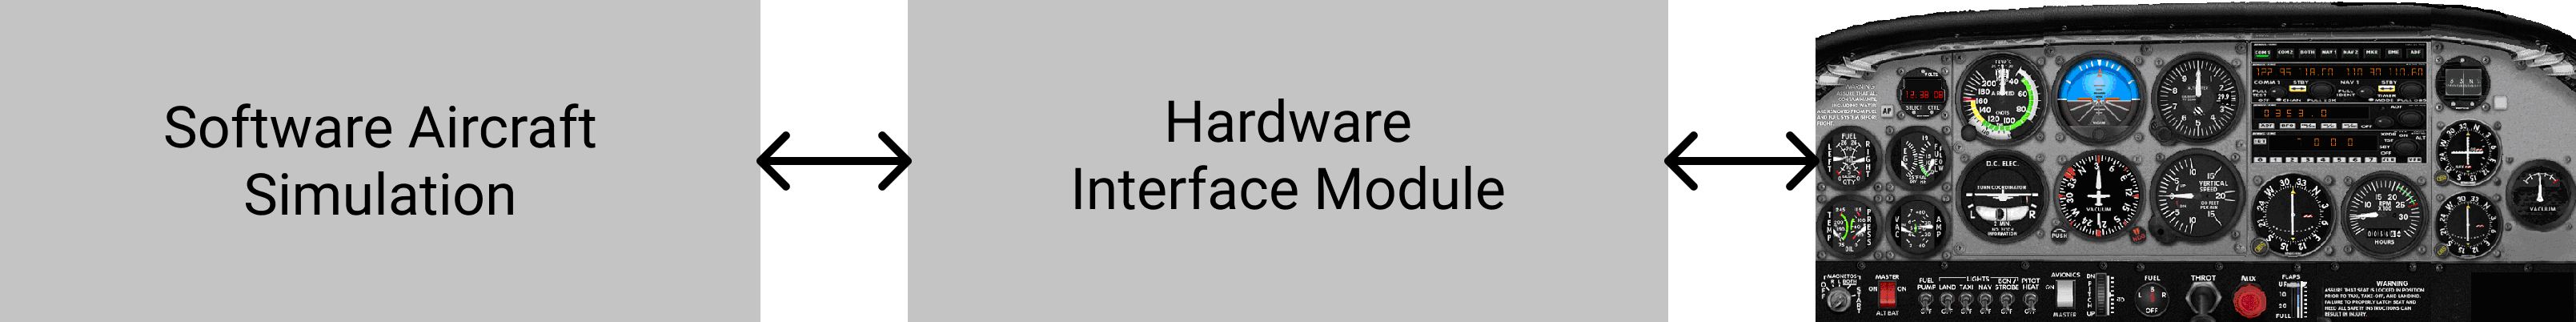
\includegraphics[width=0.6\linewidth]{img/MPIC.png}
            \caption{MPIC Interface System Overview Software Module}
        \end{figure}
        \begin{figure}[H]
            \centering
            \includegraphics[width=0.6\linewidth]{img/simulator-support-system.png}
            \caption{Simulator Support Systems}
        \end{figure}

\section{Interface System Architecture}
    \subsection{Architecture Overview}
        To meet the A661 standard used by CAE, we must seperate the User Application (UA) from the Cockpit Display System (CDS). 
        In other words, the appearance and contents of an object (Widget) on the display must be segregated from its functional 
        behavior as this is managed by the UA. As a result, the system structure can be divided into two main modules, as shown 
        in below figure, specifically the PC where the simulator sends all the data to be processed by the UA, and the CAE-MPIC 
        where the graphics rendering is performed. \\ 
        \vspace{3mm}
        To make things simple we choose to categorize the architecture into four modules:
        \begin{itemize}
            \item The UA
            \item The CDS 
            \item The Window Manager UA
            \item The communication protocol ARINC 661/DUP
        \end{itemize}
        \begin{figure}[H]
            \centering
            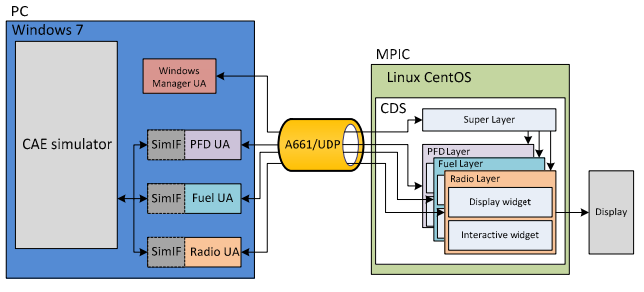
\includegraphics[width=0.6\linewidth]{img/UA.PNG}
            \caption{System Architecture}
        \end{figure}
    \subsection{What Is ARINC 661?}
        ARINC 661 is a standard which aims to normalize the definition of a \textbf{C}ockpit \textbf{D}isplay \textbf{S}ystem (CDS), 
        and the communication between the CDS and User Applications (UA) which manage aircraft avionics functions. The GUI definition 
        is completely defined in binary \textbf{D}efinition \textbf{F}iles (DF).\\
        \vspace{3mm}
        The CDS software is constituted of a kernel which is able to create the GUI hierarchy specified in the DF during initialization, 
        thus not needing to be recompiled if the GUI definition changes. \\
        \vspace{3mm}
        The standard normalizes: 
        \begin{itemize}
            \item the GUI definition of the CDS interface, in a binary file called DF (Definition File) defining the structure of the 
            graphical interface tree. The GUI tree is instantiated at initialization time (called the Definition Phase in the standard) 
            in the CDS, using the definition contained in the DF;
            \item the communication at runtime between the User Applications (UA) and the CDS. This communication protocol is typically 
            used for UAs to send widgets modifications to the CDS, and return user events (such as buttons selection) from CDS to UA.
        \end{itemize}
        In order to be compliant with the standard, a CDS must have a kernel that can create the widgets tree during CDS initialization, 
        using the Definition File, and communicate with UA in both ways using the runtime protocol. \\ 
        \vspace{3mm}
        ARINC 661 does not imply the use of a particular Data bus structure to perform the low-level communication between CDS and UA. 
        For example, an ARINC 429 or Ethernet protocol such as ARINC 664 can be used, but it is not mandatory. \\ 
        \subsubsection{GUI Structure}
            \begin{itemize}
                \item The \textbf{Cockpit Display System (CDS)} is the graphic Server which is responsible to show and manage the GUI;
                \item A \textbf{User Application (UA)} is one system application which communicates with the CDS. The CDS manage one ore more 
                Definition Files for each User Application. At run-time, messages are exchanged between UAs and the CDS;
                \item A \textbf{Definition File (DF)} specifies the GUI definition associated with one User Application (note that a User 
                Application may be associated by more than one DF). A Definition File contains the definition of one or more Layers;
                \item A Layer (also named User Application Layer Definition or \textbf{UALD}) is a GUI container for widgets;
                \item A widget is the basic building block of the GUI
            \end{itemize}
            \begin{figure}[H]
                \centering
                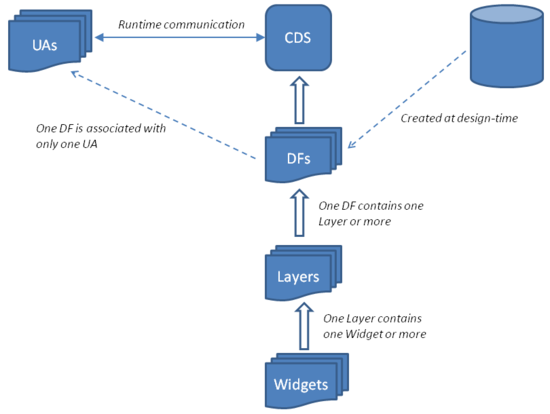
\includegraphics[width=0.6\linewidth]{img/ARINC_661_structure.png}
                \caption{ARINC 661 structure}
            \end{figure}
        \subsubsection{GUI Definition}
            Each DF binary file specifies the GUI definition for one User Application (UA) User interface. Several UA user interface trees can 
            be combined to constitute the CDS display definition. \\
            \vspace{3mm}
            A DF is composed of two parts : an optional symbol definition, and a widgets definition. The widget library is similar to Widgets 
            used in computing. There are Containers, Lists, ScrollPanes, Buttons, Menus, Labels, EditBoxes, etc... \\
            \vspace{3mm}
            Although the DF File is binary, the standard has also defined an associated XML definition, which is easier to manipulate in tools.
    \subsection{User Application}
        The UA contains the logic for each CDS. There are three generic CDSs are developed:
        \begin{itemize}
            \item Primary Flight Display (PFD)
            \item Fuel page
            \item Radio page
        \end{itemize}
        Each CDS is controlled by a UA. The main task for each UA is to update the widget's paremeters by sending precisely defined 
        ARINC 661 messages to the CDS. The UA uses the simulator global variables such as speed, altitude, heading, etc., through a 
        tailored simulator interface called SimIF, to build the message for the CDS. SimIF is a library that enables the UA to write 
        and read simulator variables to and from the shared memory, which contains the global variables that the simulator needs to 
        run its applications, including the PFD, fuel and radio variables.
    \subsection{Cockpit Display System}
        The CDS is made up of a number of Layers controlled by one UA. In A661, a Layer is the highest entity of the CDS as seen by 
        the UA. From a CDS viewpoint, a Layer is a graphical entity related to the application within a window page. Layers are numbered 
        and can be connected to a SuperLayer. Each Layer contains several widgets that are displayed as objects. The SuperLayer links all 
        UA Layers for the flight deck together by a single CDS Layer. The SuperLayer also uses standard widgets, to define all of the 
        groupings of functional UA Layers that are needed to draw each display and uses connectors to reference those functional UA 
        Layers as shown in below figure.
        \begin{figure}[H]
            \centering
            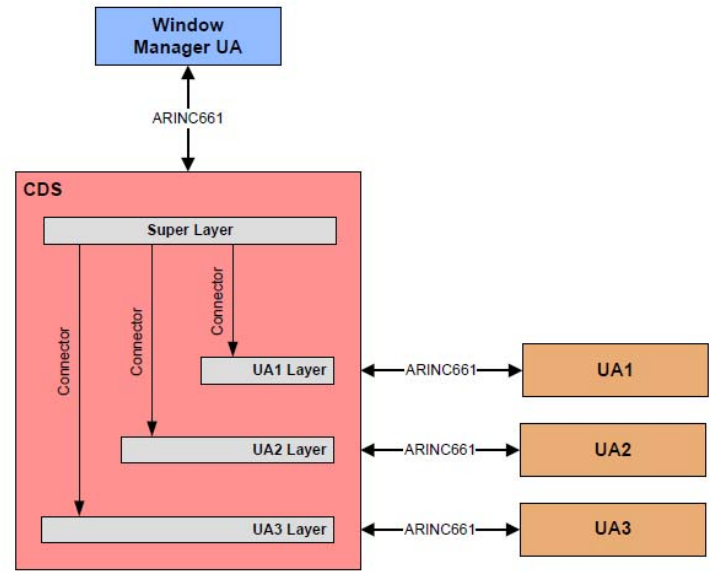
\includegraphics[width=0.6\linewidth]{img/SuperLayer.PNG}
            \caption{Super layer}
        \end{figure}
        This figure shows a Display Unit that has a set of windows, and each window is subdivided in a number of layers, which are owned 
        by their respective UA.
        \begin{figure}[H]
            \centering
            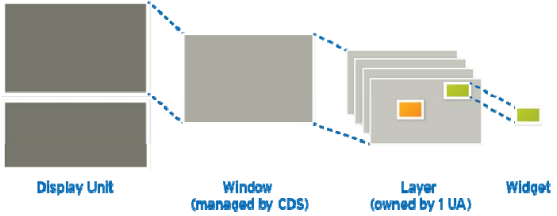
\includegraphics[width=0.6\linewidth]{img/window-layer.PNG}
            \caption{Window \& Layer illustration}
        \end{figure}
    \subsection{Window Manager}
        The Window Manager’s primary task is to manage all the logical display of each CDS page as well as the page’s selection interface, 
        for the user to control \textbf{(CDS+UA)}.


\section{Interface panels power and requirements}
    \subsection{Simulation Interfacing Concepts}
        Figure shownws a typical power, lighting and interface signal requirements to drive an aircraft and simulated instruments/panels.
        \begin{figure}[H]
            \centering
            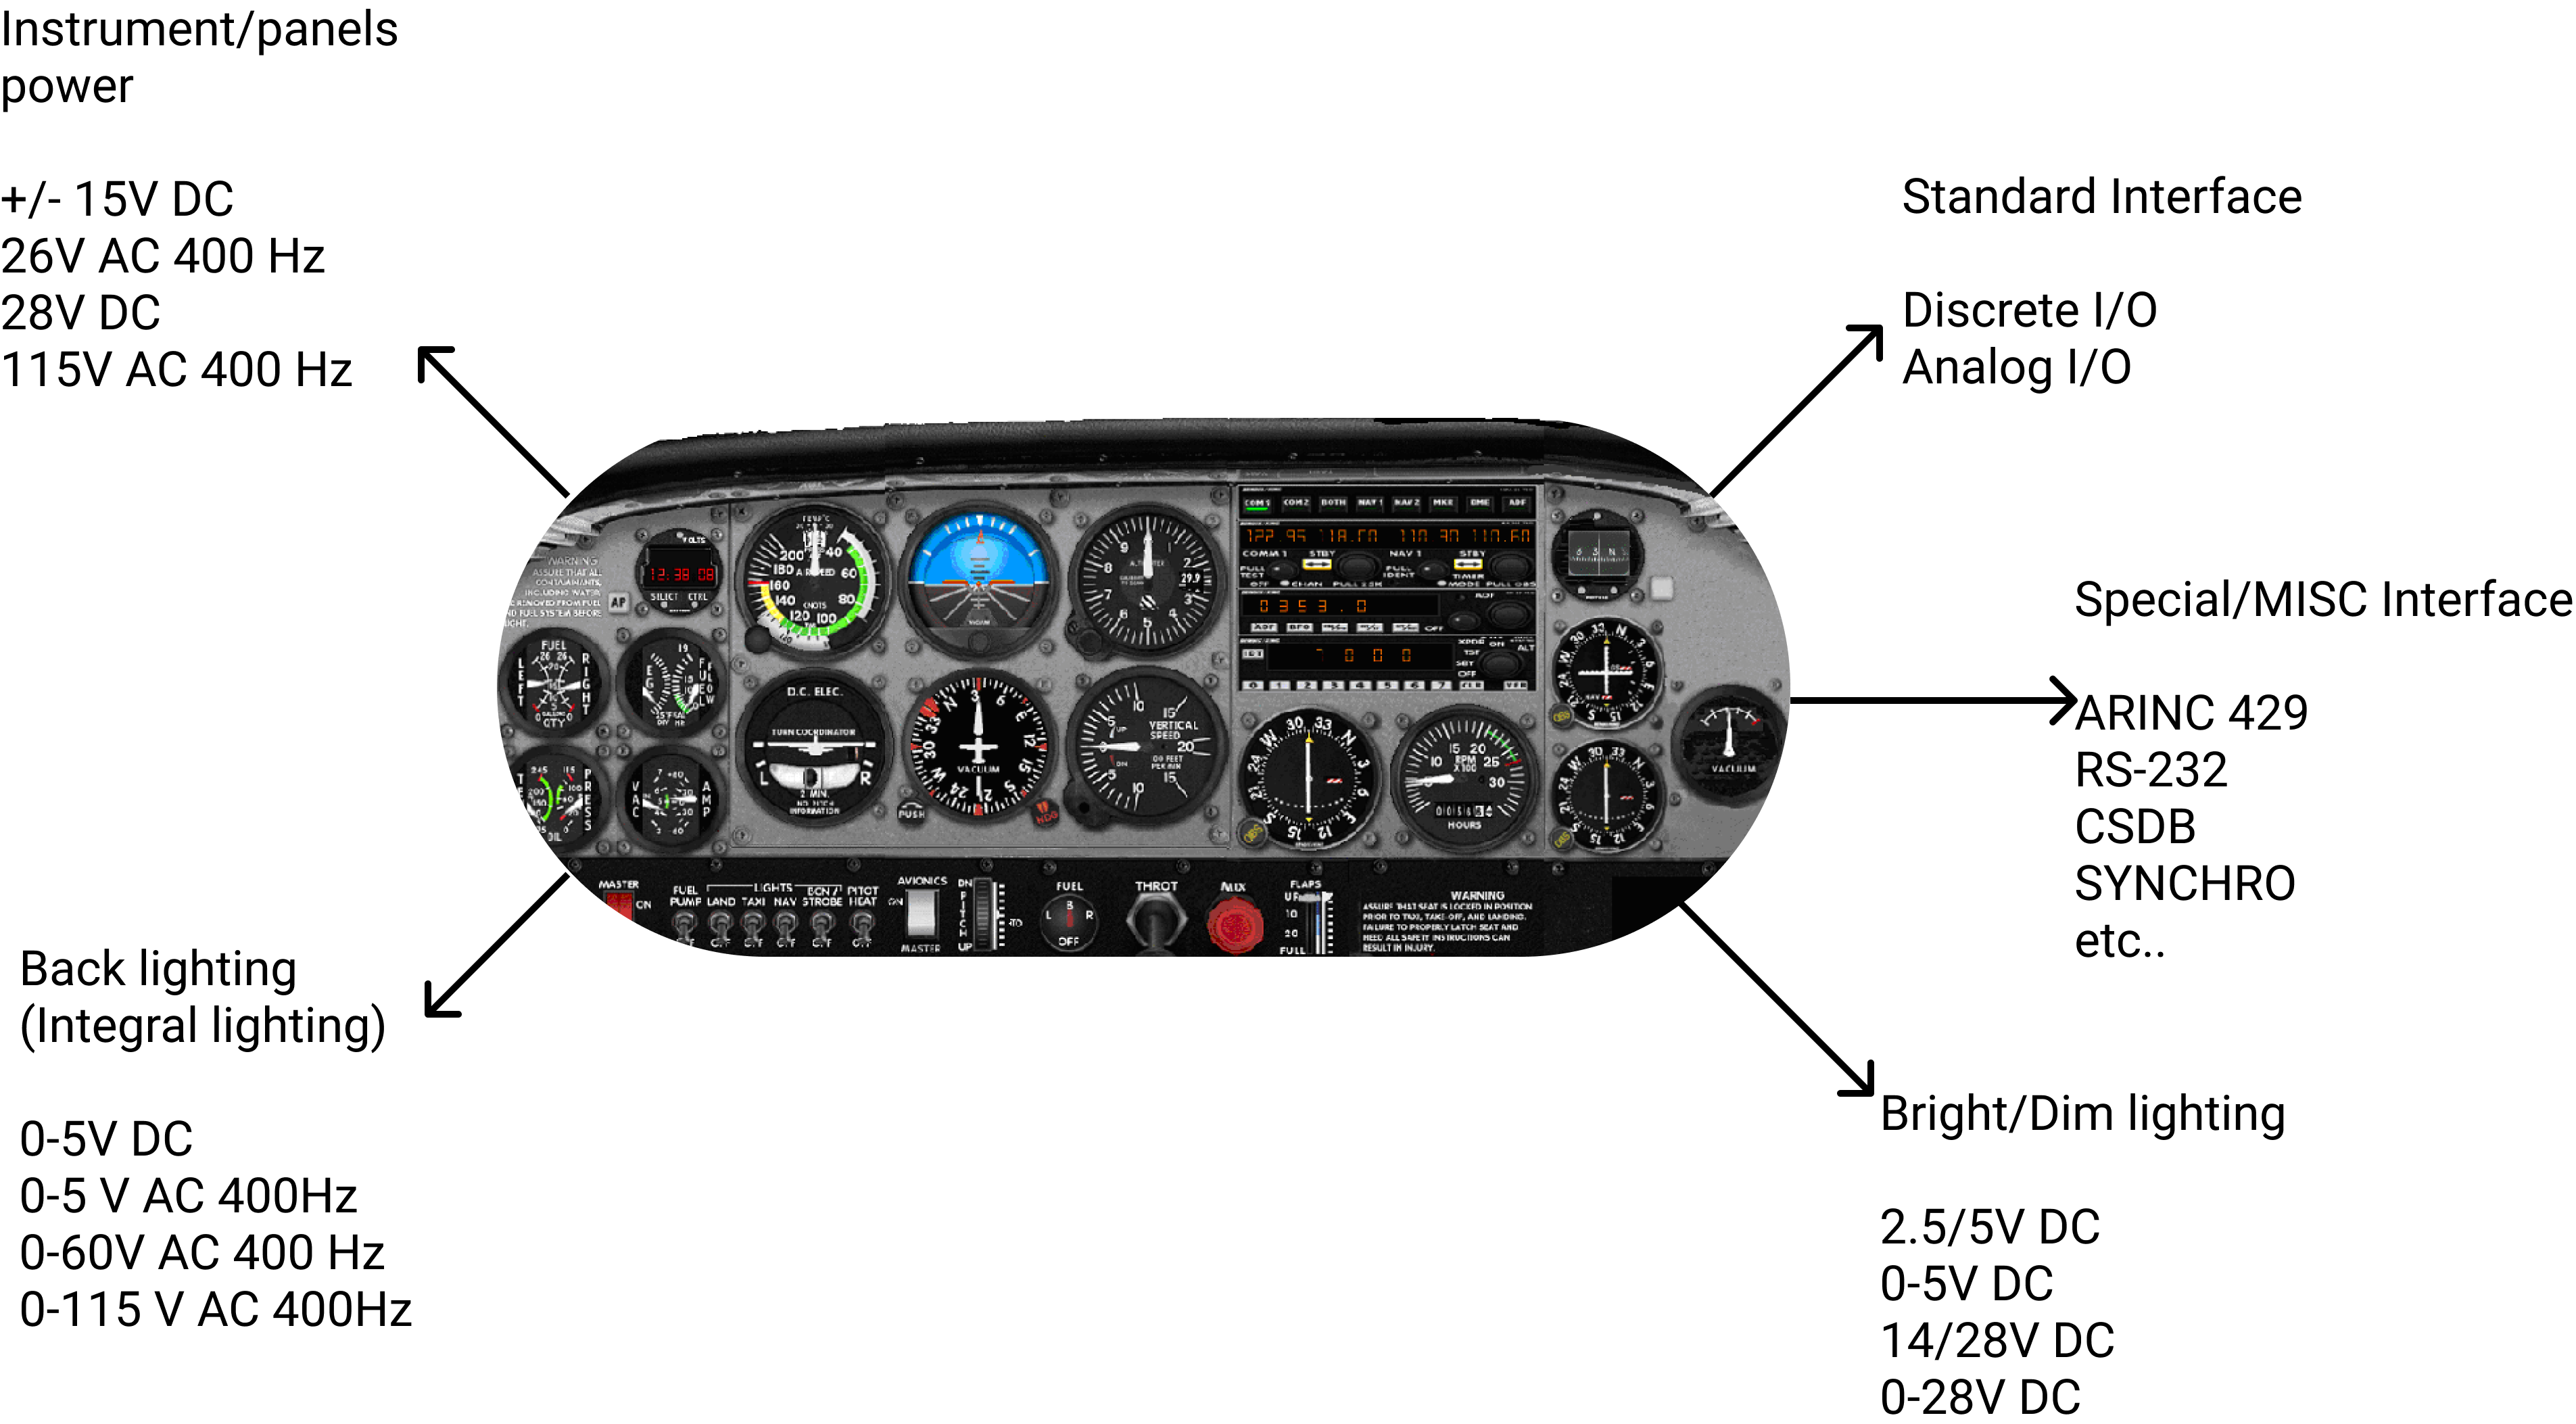
\includegraphics[width=0.6\linewidth]{img/Simulation.png}
            \caption{Aircraft panels power interface requirements}
        \end{figure}
        This figure is shown the Interface Systems Architecture.
        \begin{figure}[H]
            \centering
            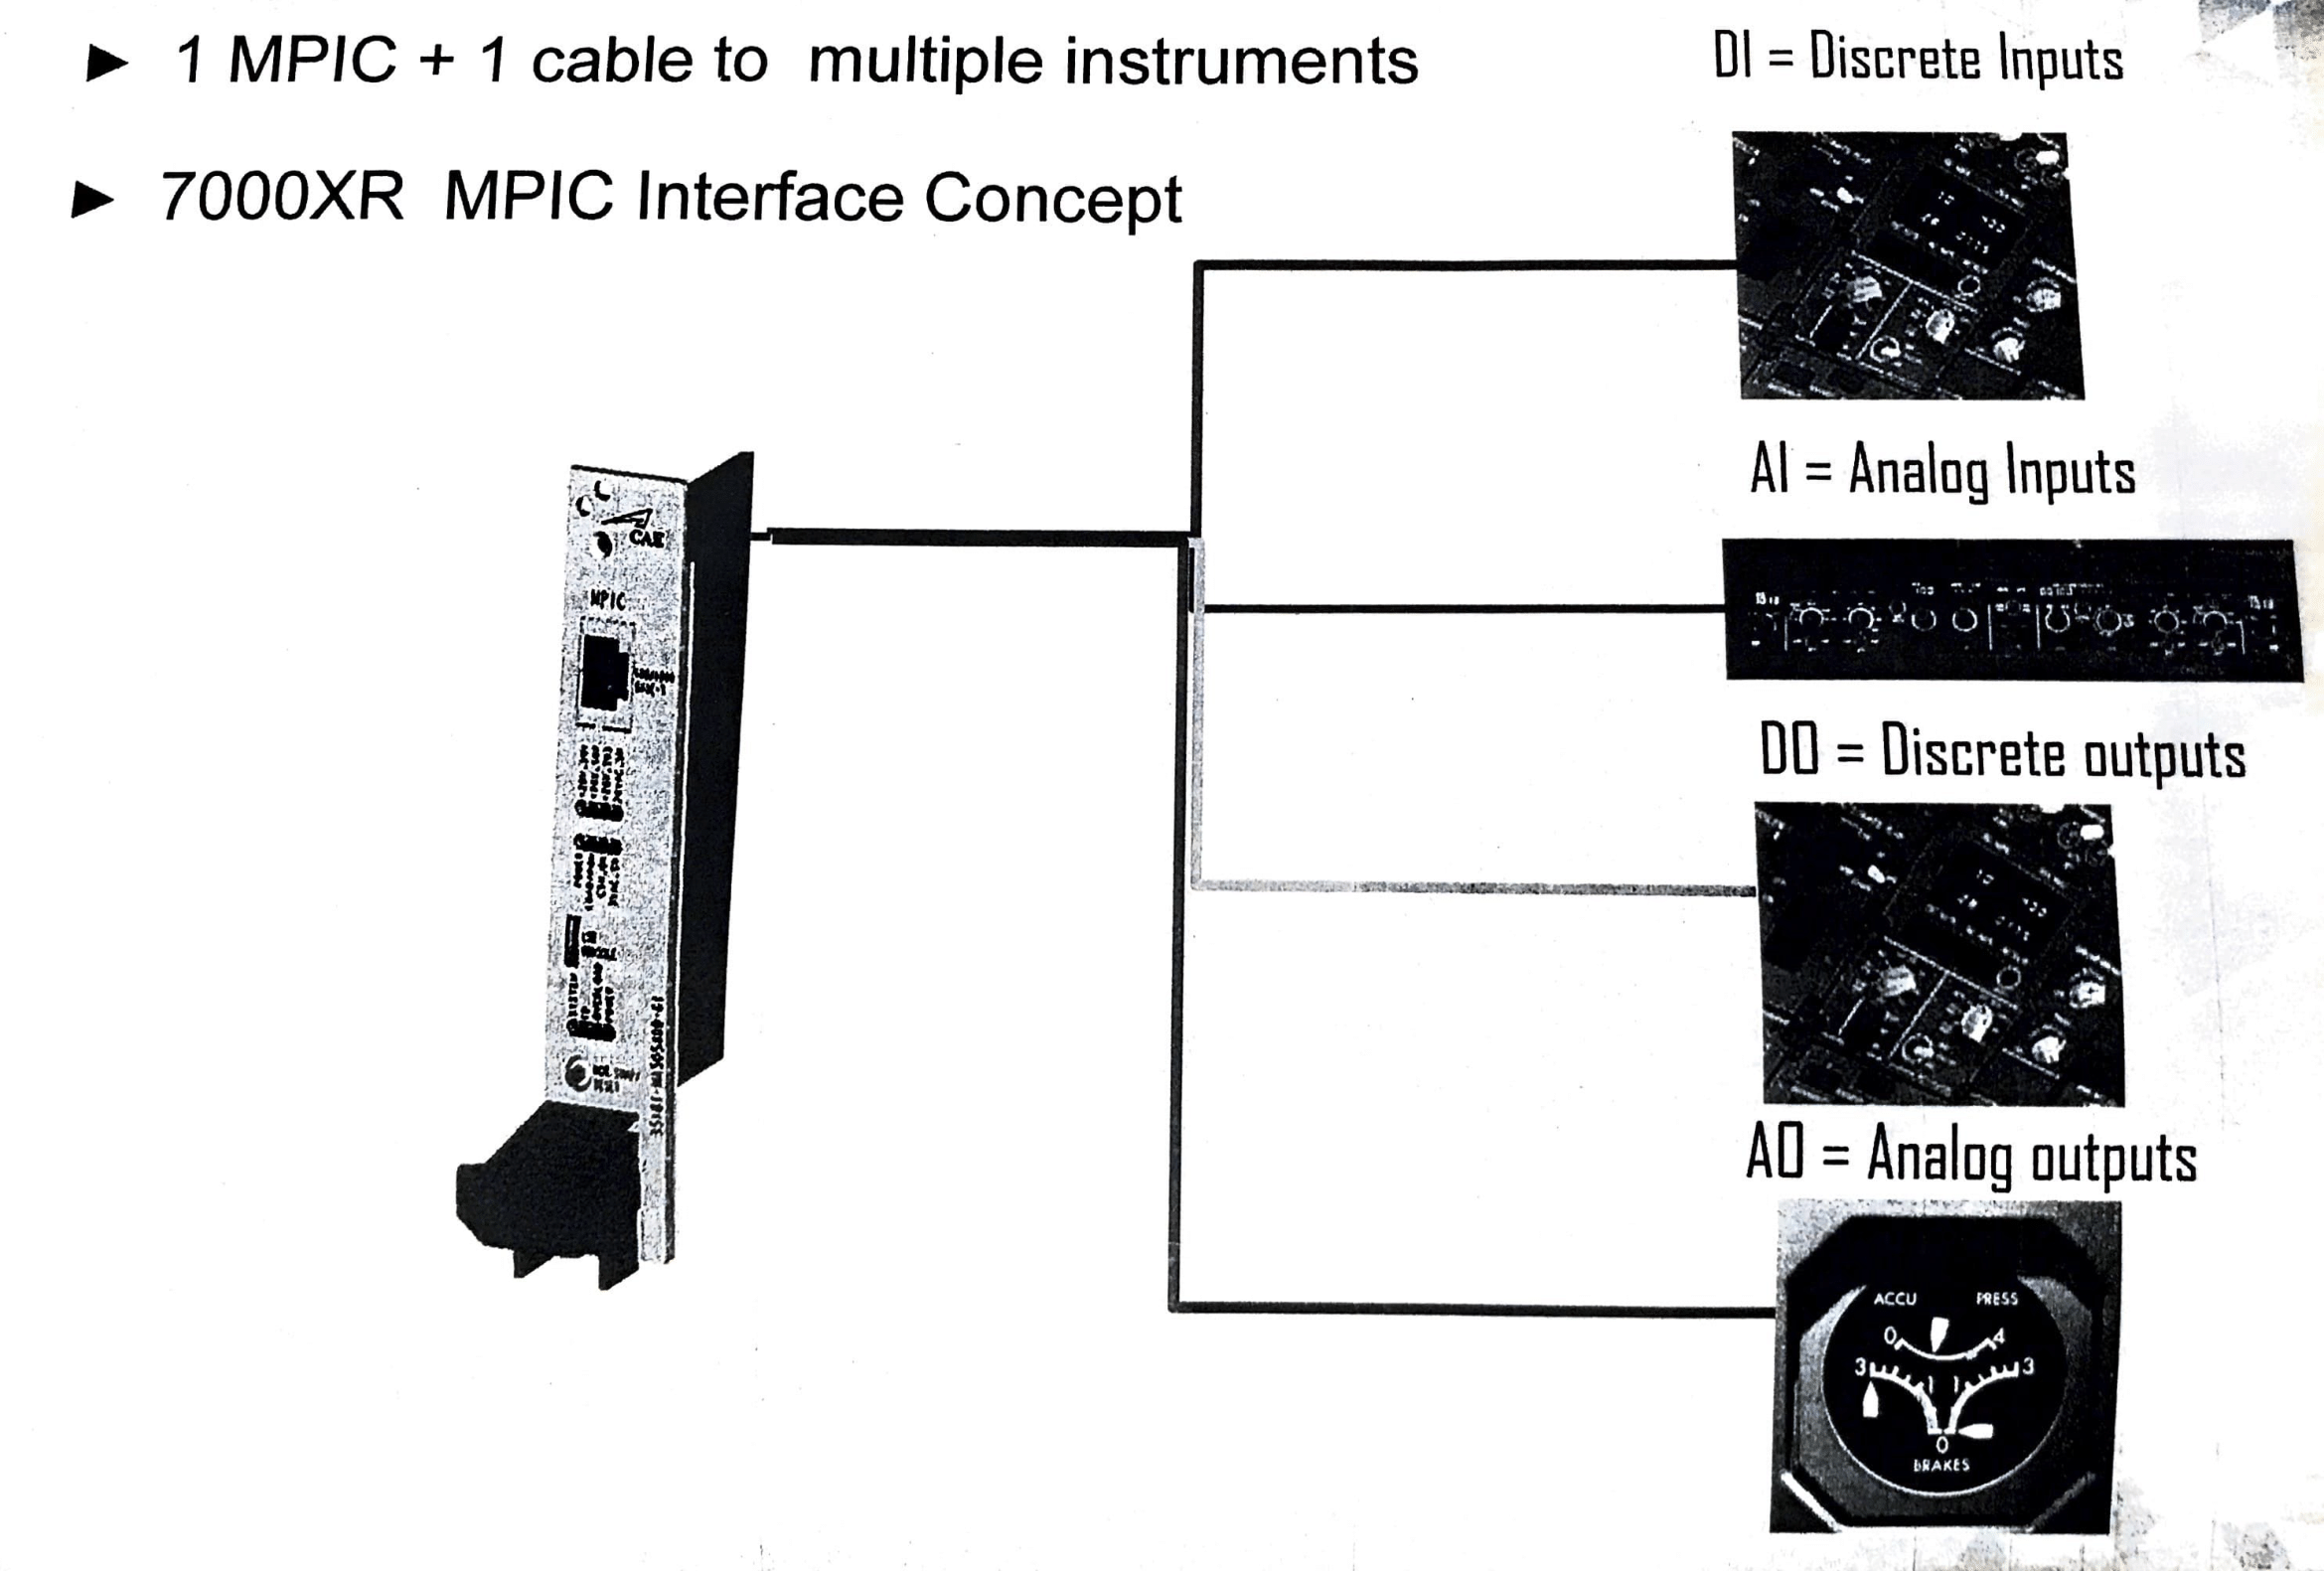
\includegraphics[width=0.6\linewidth]{img/image.png}
            \caption{Interface systems architecture}
        \end{figure}
        Figure below here shows an actual typical aircraft wiring diagram for a lighting functionality.
        \begin{itemize}
            \item A switch (SW) turns the lamp on/off;
            \item A circuit breaker (CB) powers the bus;
            \item Lamp could be for reading, map utility light or annunciator light switch.
        \end{itemize}
        \begin{figure}[H]
            \centering
            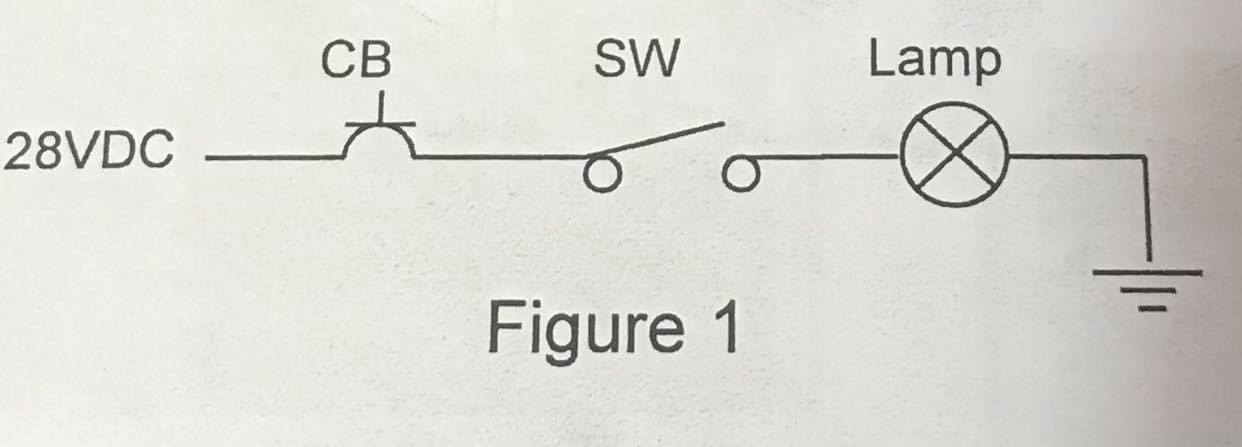
\includegraphics[width=0.6\linewidth]{img/figure1.jpg}
            \caption{Wiring diagram for lighting functionality}
        \end{figure}
        And the typical interface simulation wiring includes:
        \begin{itemize}
            \item The DIP GND on the MPIC senses the status (on/off) of a switch (SW) or a circuit breaker (simulated CB);
            \item DOP 28V on the MPIC turns the lamp on/off;
            \item Additional DOP 28V and DOP GND create a fault (mal-function) condition;
            \item Software simulation manages all the above actions and also occasionally broadcasts aircraft condition to other simulation 
            systems.
        \end{itemize}
        \begin{figure}[H]
            \centering
            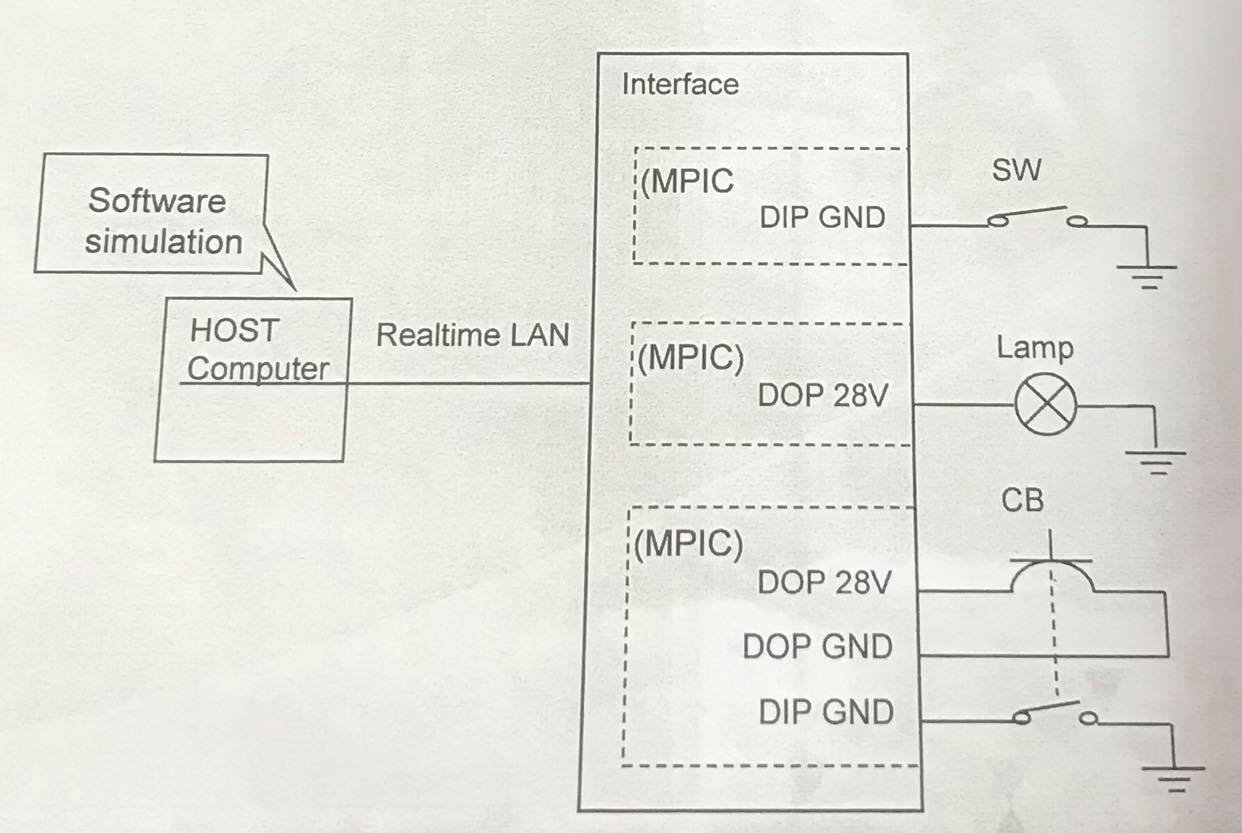
\includegraphics[width=0.6\linewidth]{img/figure2.jpg}
            \caption{Interface simulation wiring}
        \end{figure}
    \subsection{Major Components}
        \begin{figure}[H]
            \centering
            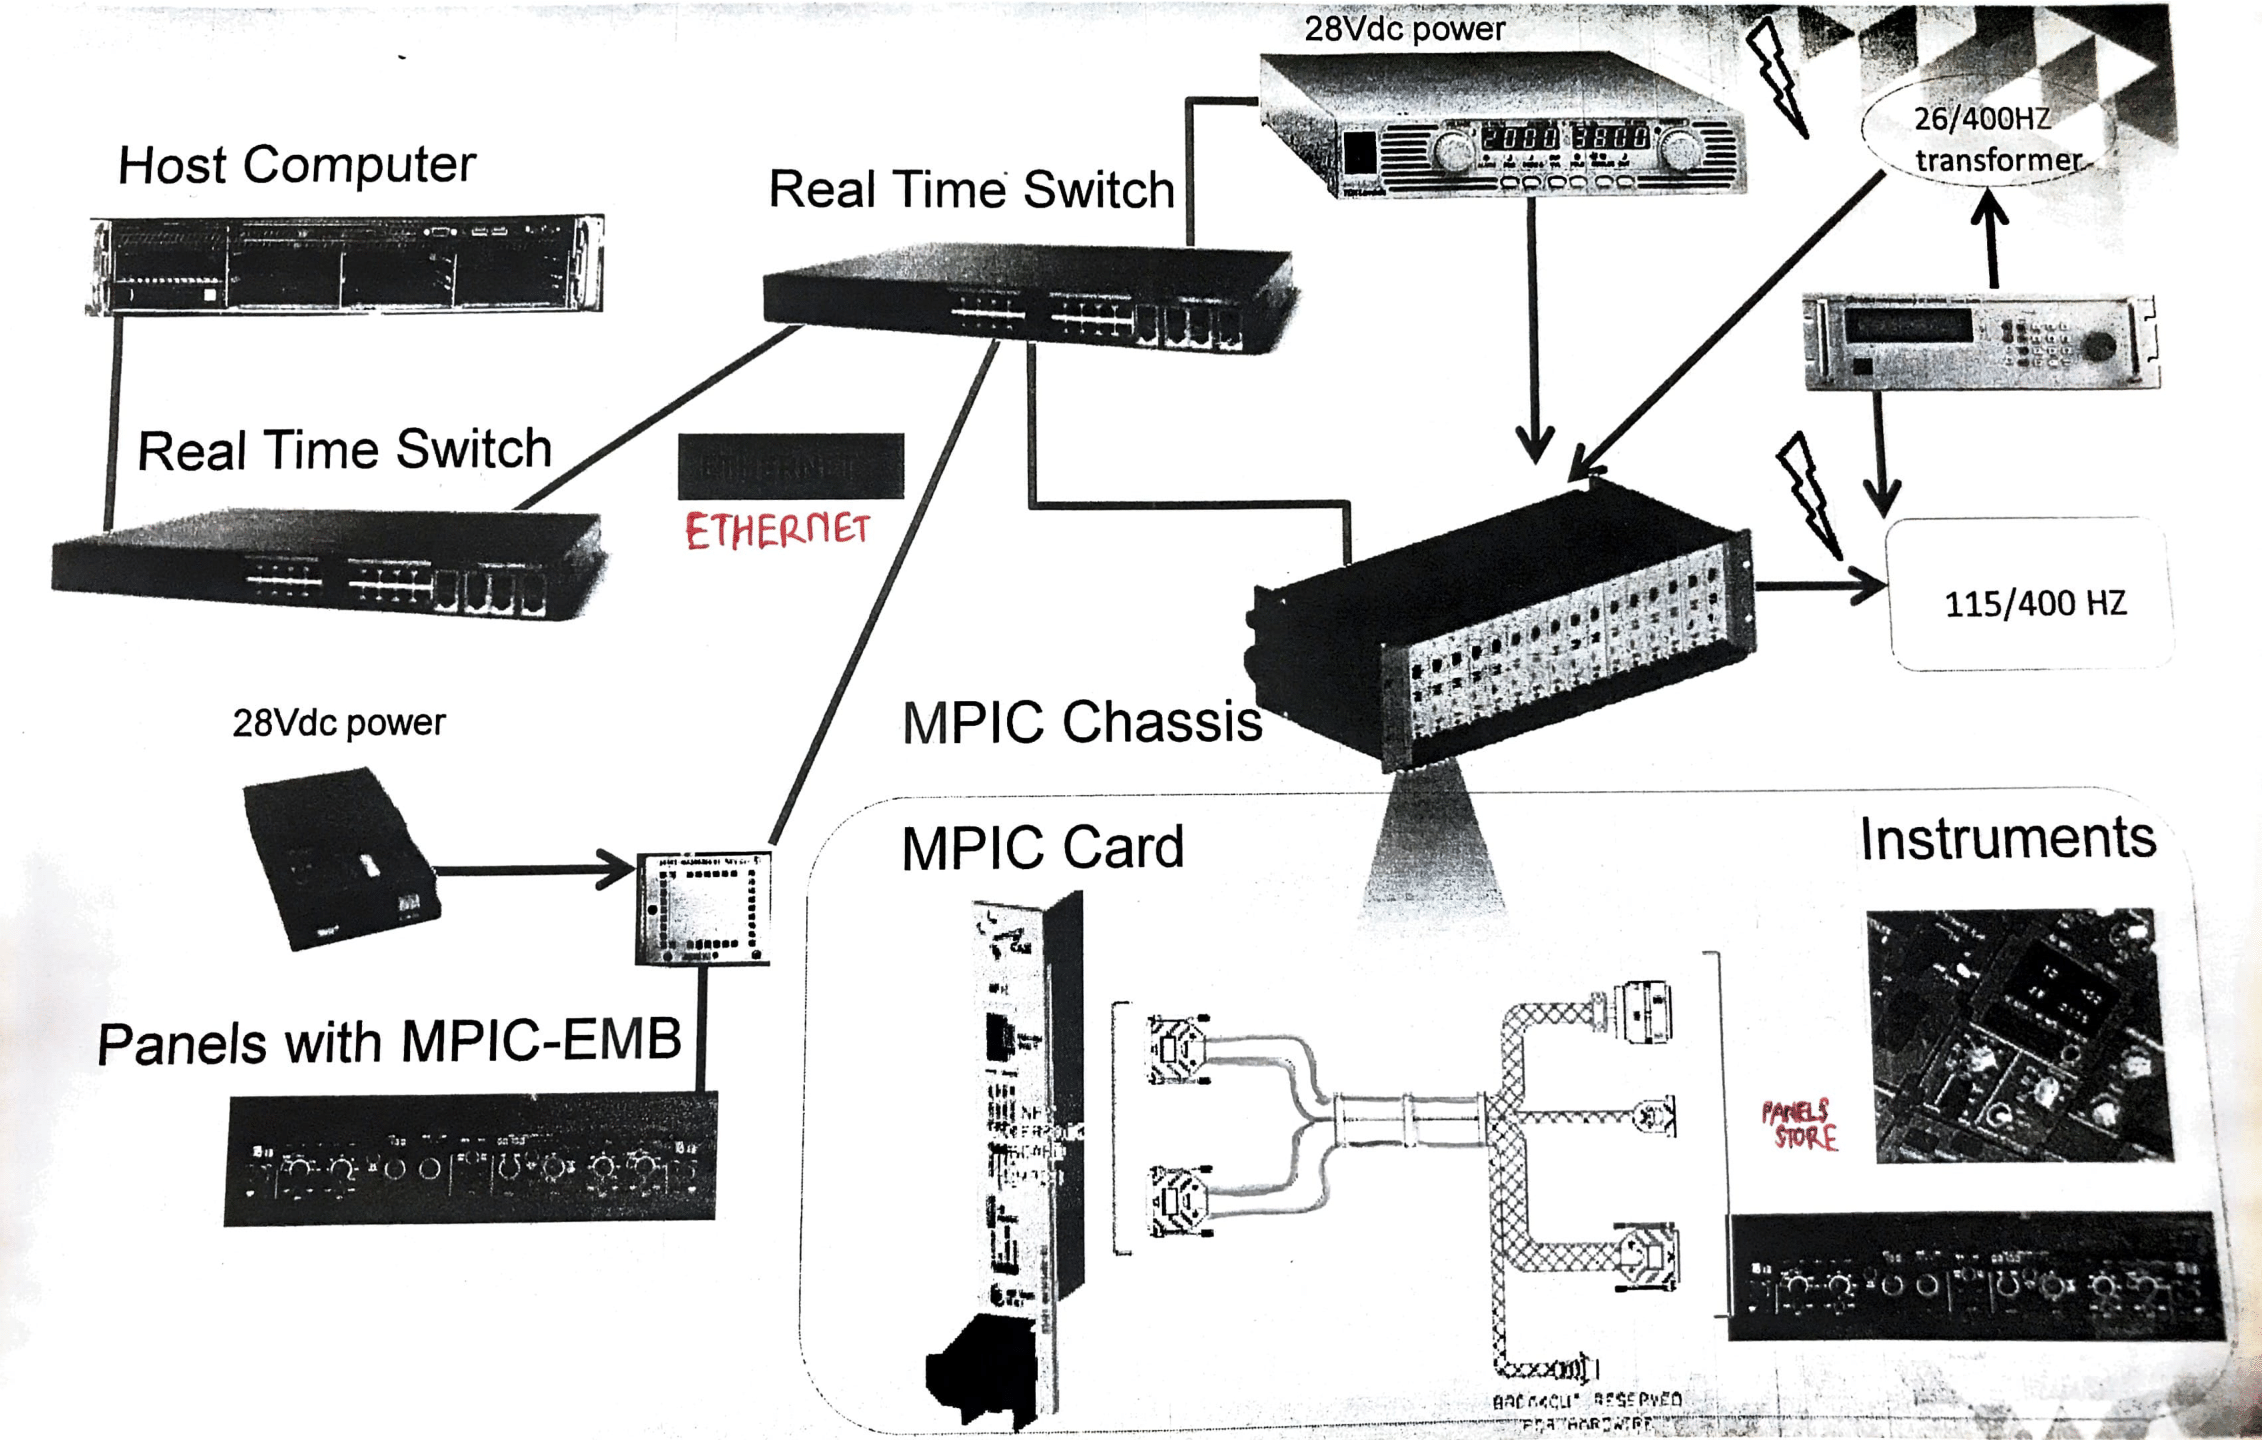
\includegraphics[width=0.6\linewidth]{img/require-component.png}
            \caption{Interface systems architecture}
        \end{figure}
        \begin{figure}[H]
            \centering
            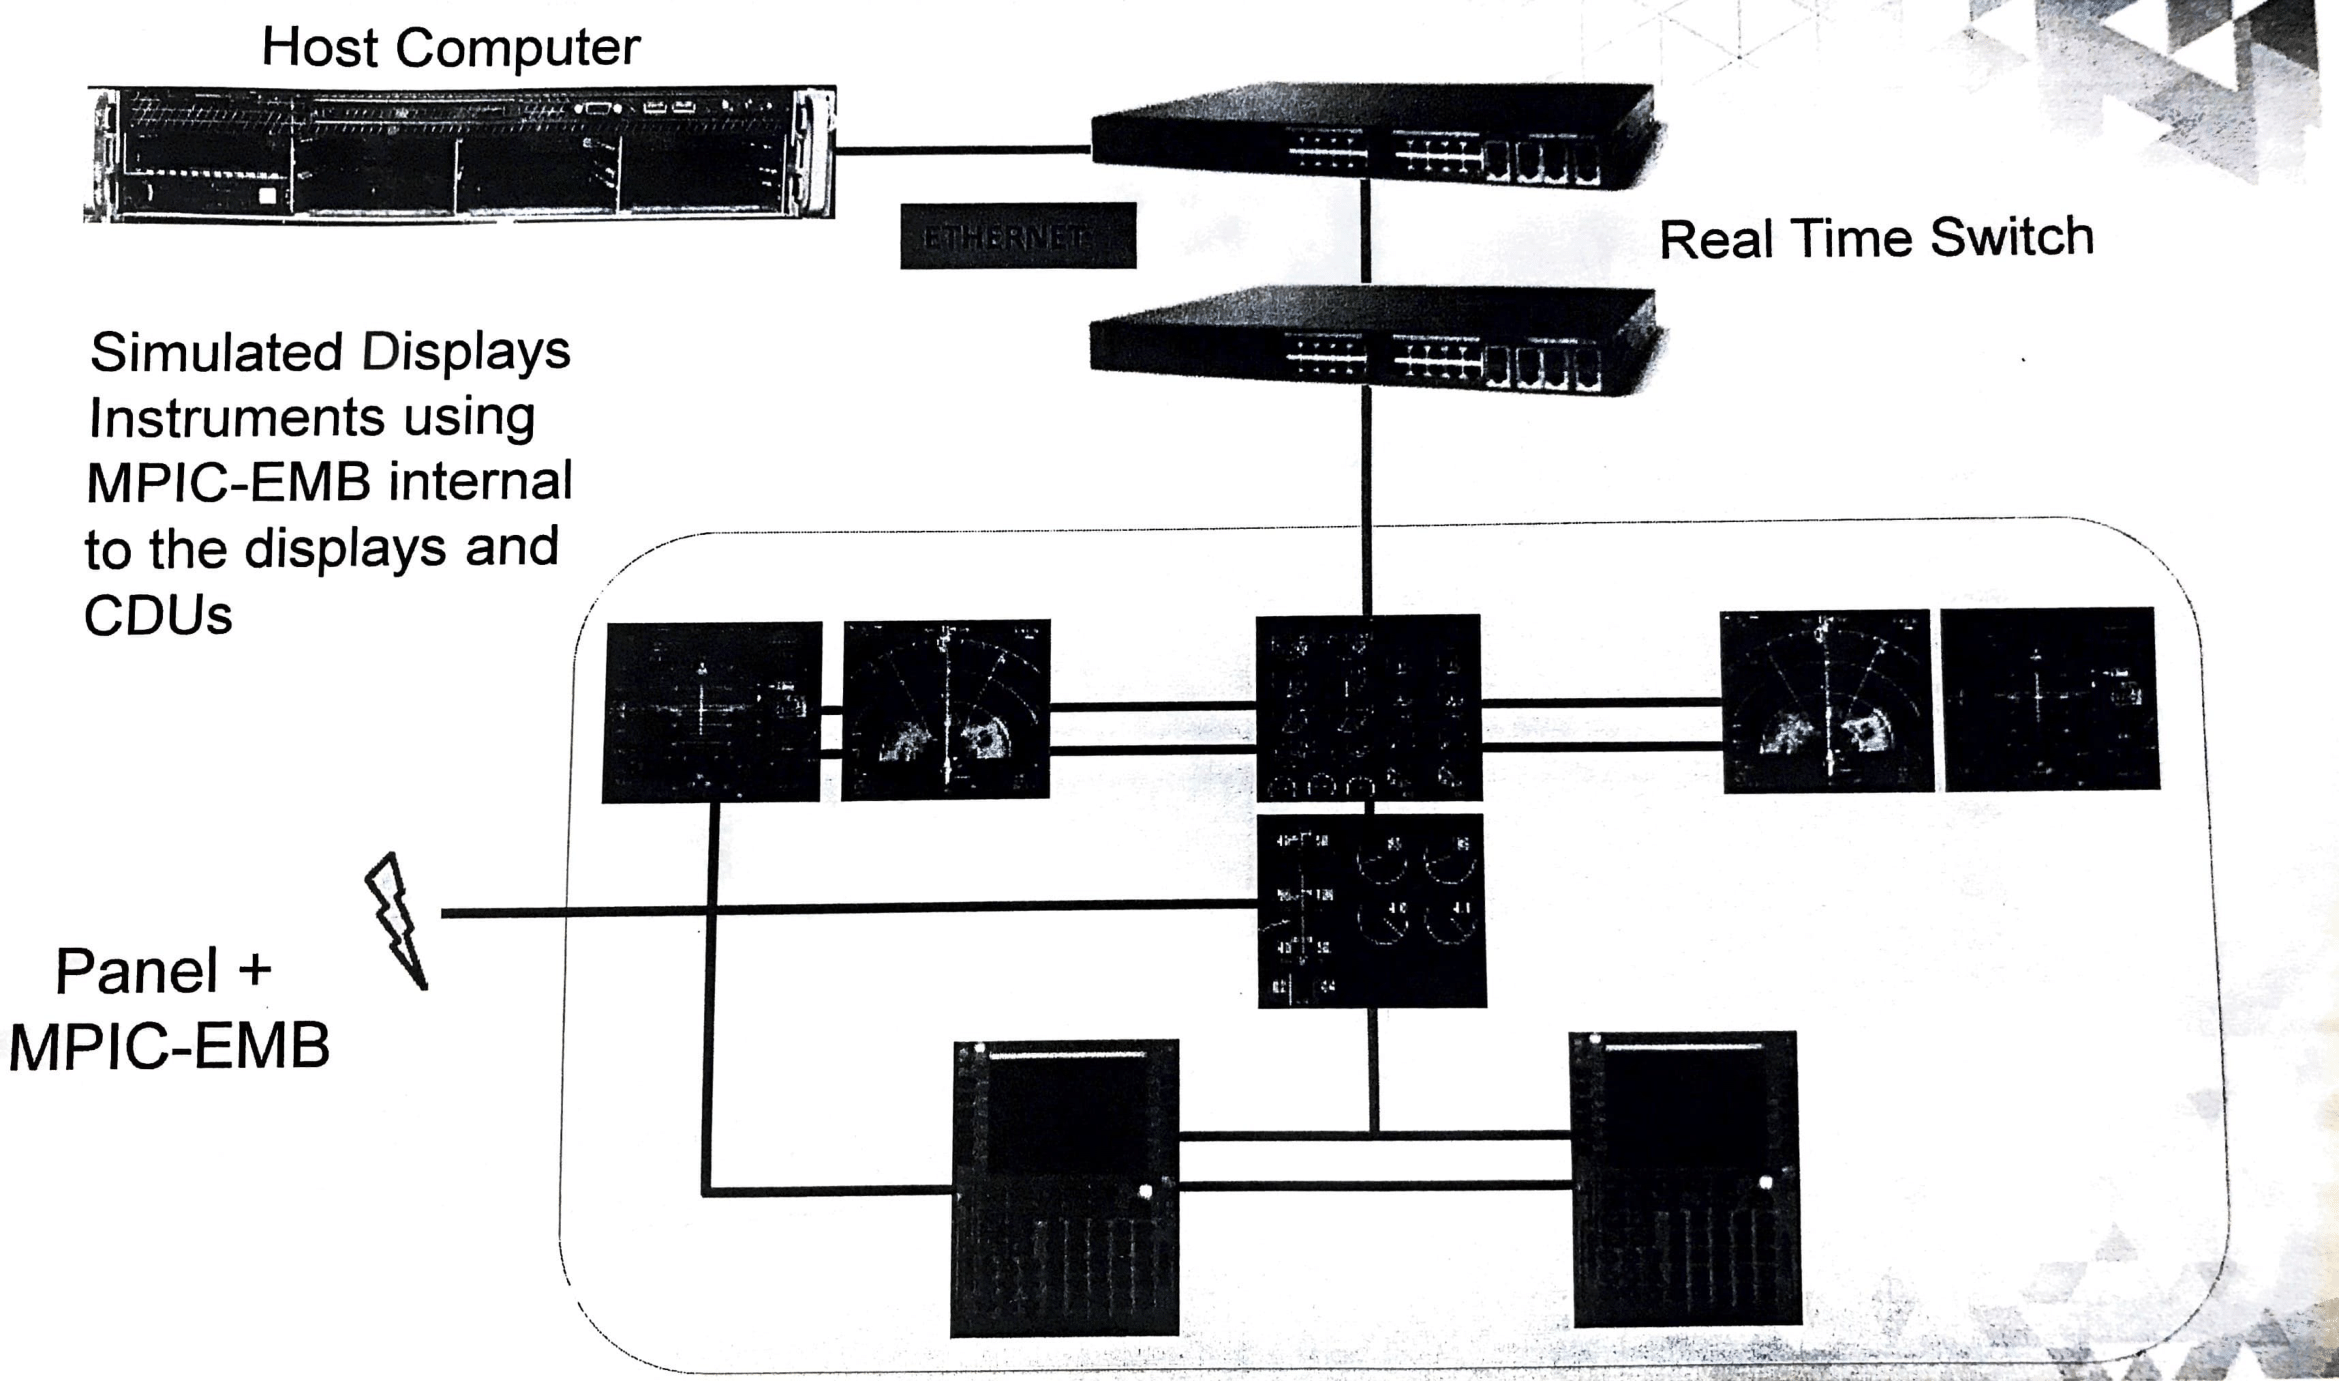
\includegraphics[width=0.6\linewidth]{img/Simulated-Display.png}
            \caption{Simulated displays instruments}
        \end{figure}
    \subsection{Network Architecture}
        \begin{figure}[H]
            \centering
            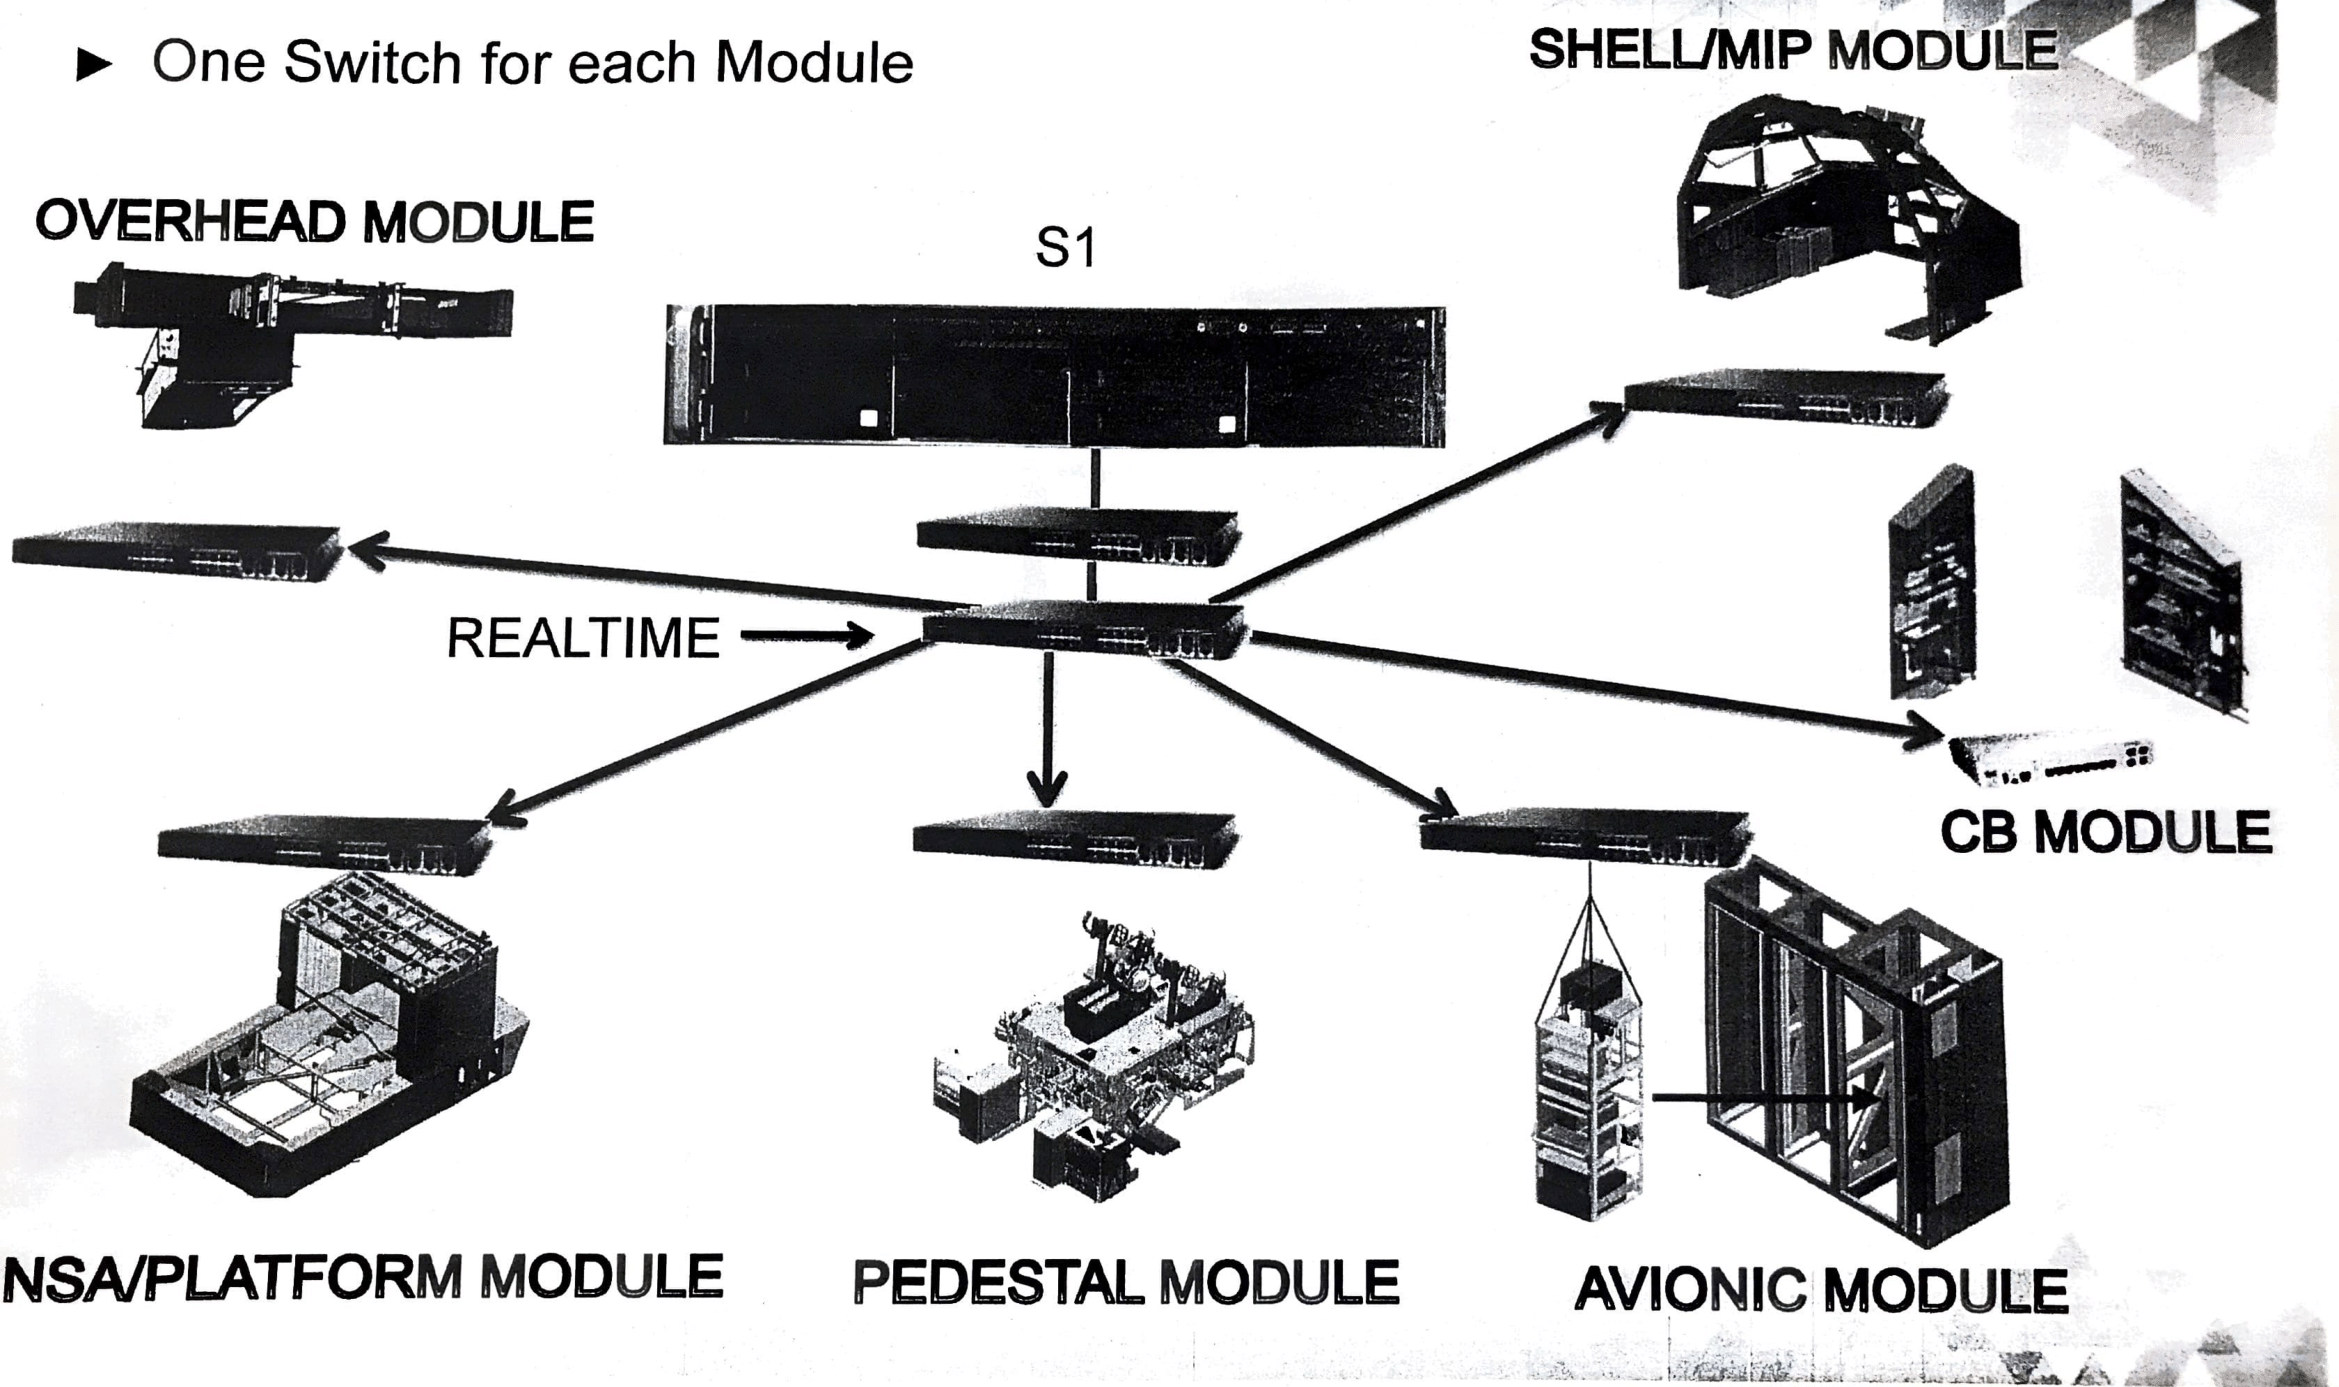
\includegraphics[width=0.6\linewidth]{img/network.png}
            \caption{Network modules}
        \end{figure}
        \subsubsection{Module Level}
            \begin{itemize}
                \item MPIC chassis is composed of 16 MPIC slots, each divided in groups of 4;
                \item Each group of 4 uses the same Ethernet cable;
                \item Each MPIC-EMB has its own cable;
                \item An Ethernet cable part of a group of 4 can be plugged into any card in that specific group.
            \end{itemize}
            \begin{figure}
                \centering
                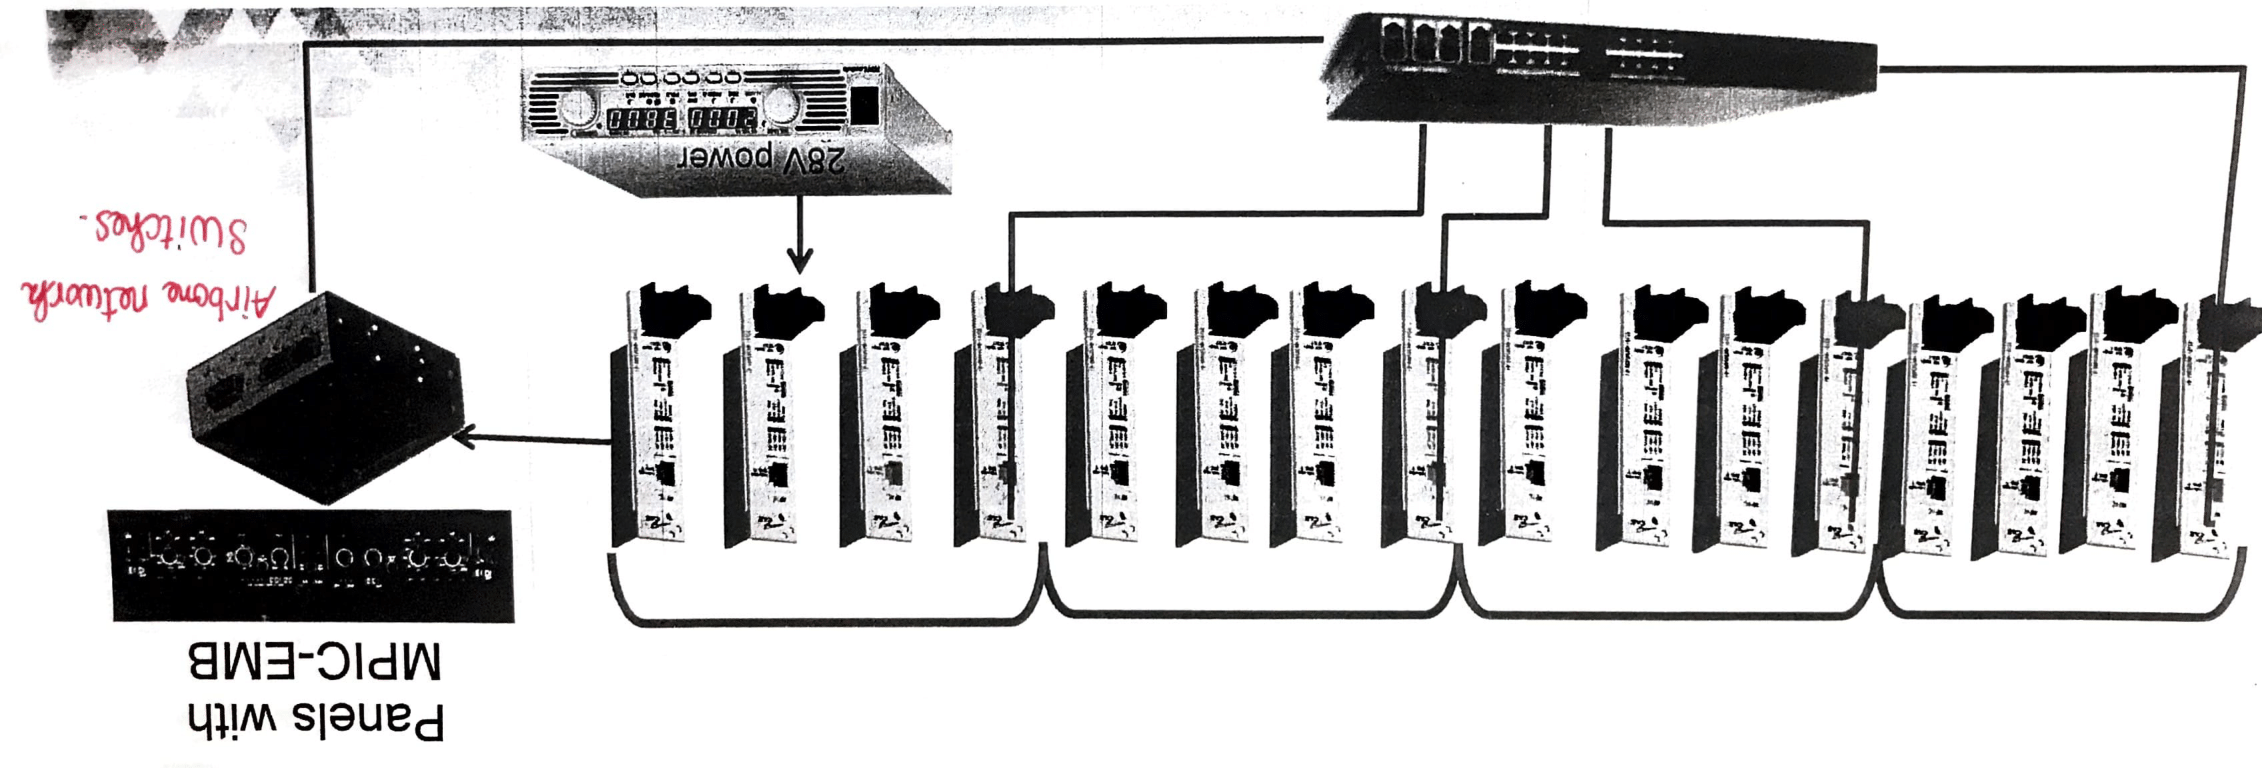
\includegraphics[width=0.6\linewidth]{img/Module-level.png}
                \caption{Module level network}
            \end{figure}
    \subsection{Communication Paths}
        Interface cards are connected to the Real time LAN. \\ 
        \vspace{3mm}
        Real time LAN is extended on the backplane.
        \begin{figure}[H]
            \centering
            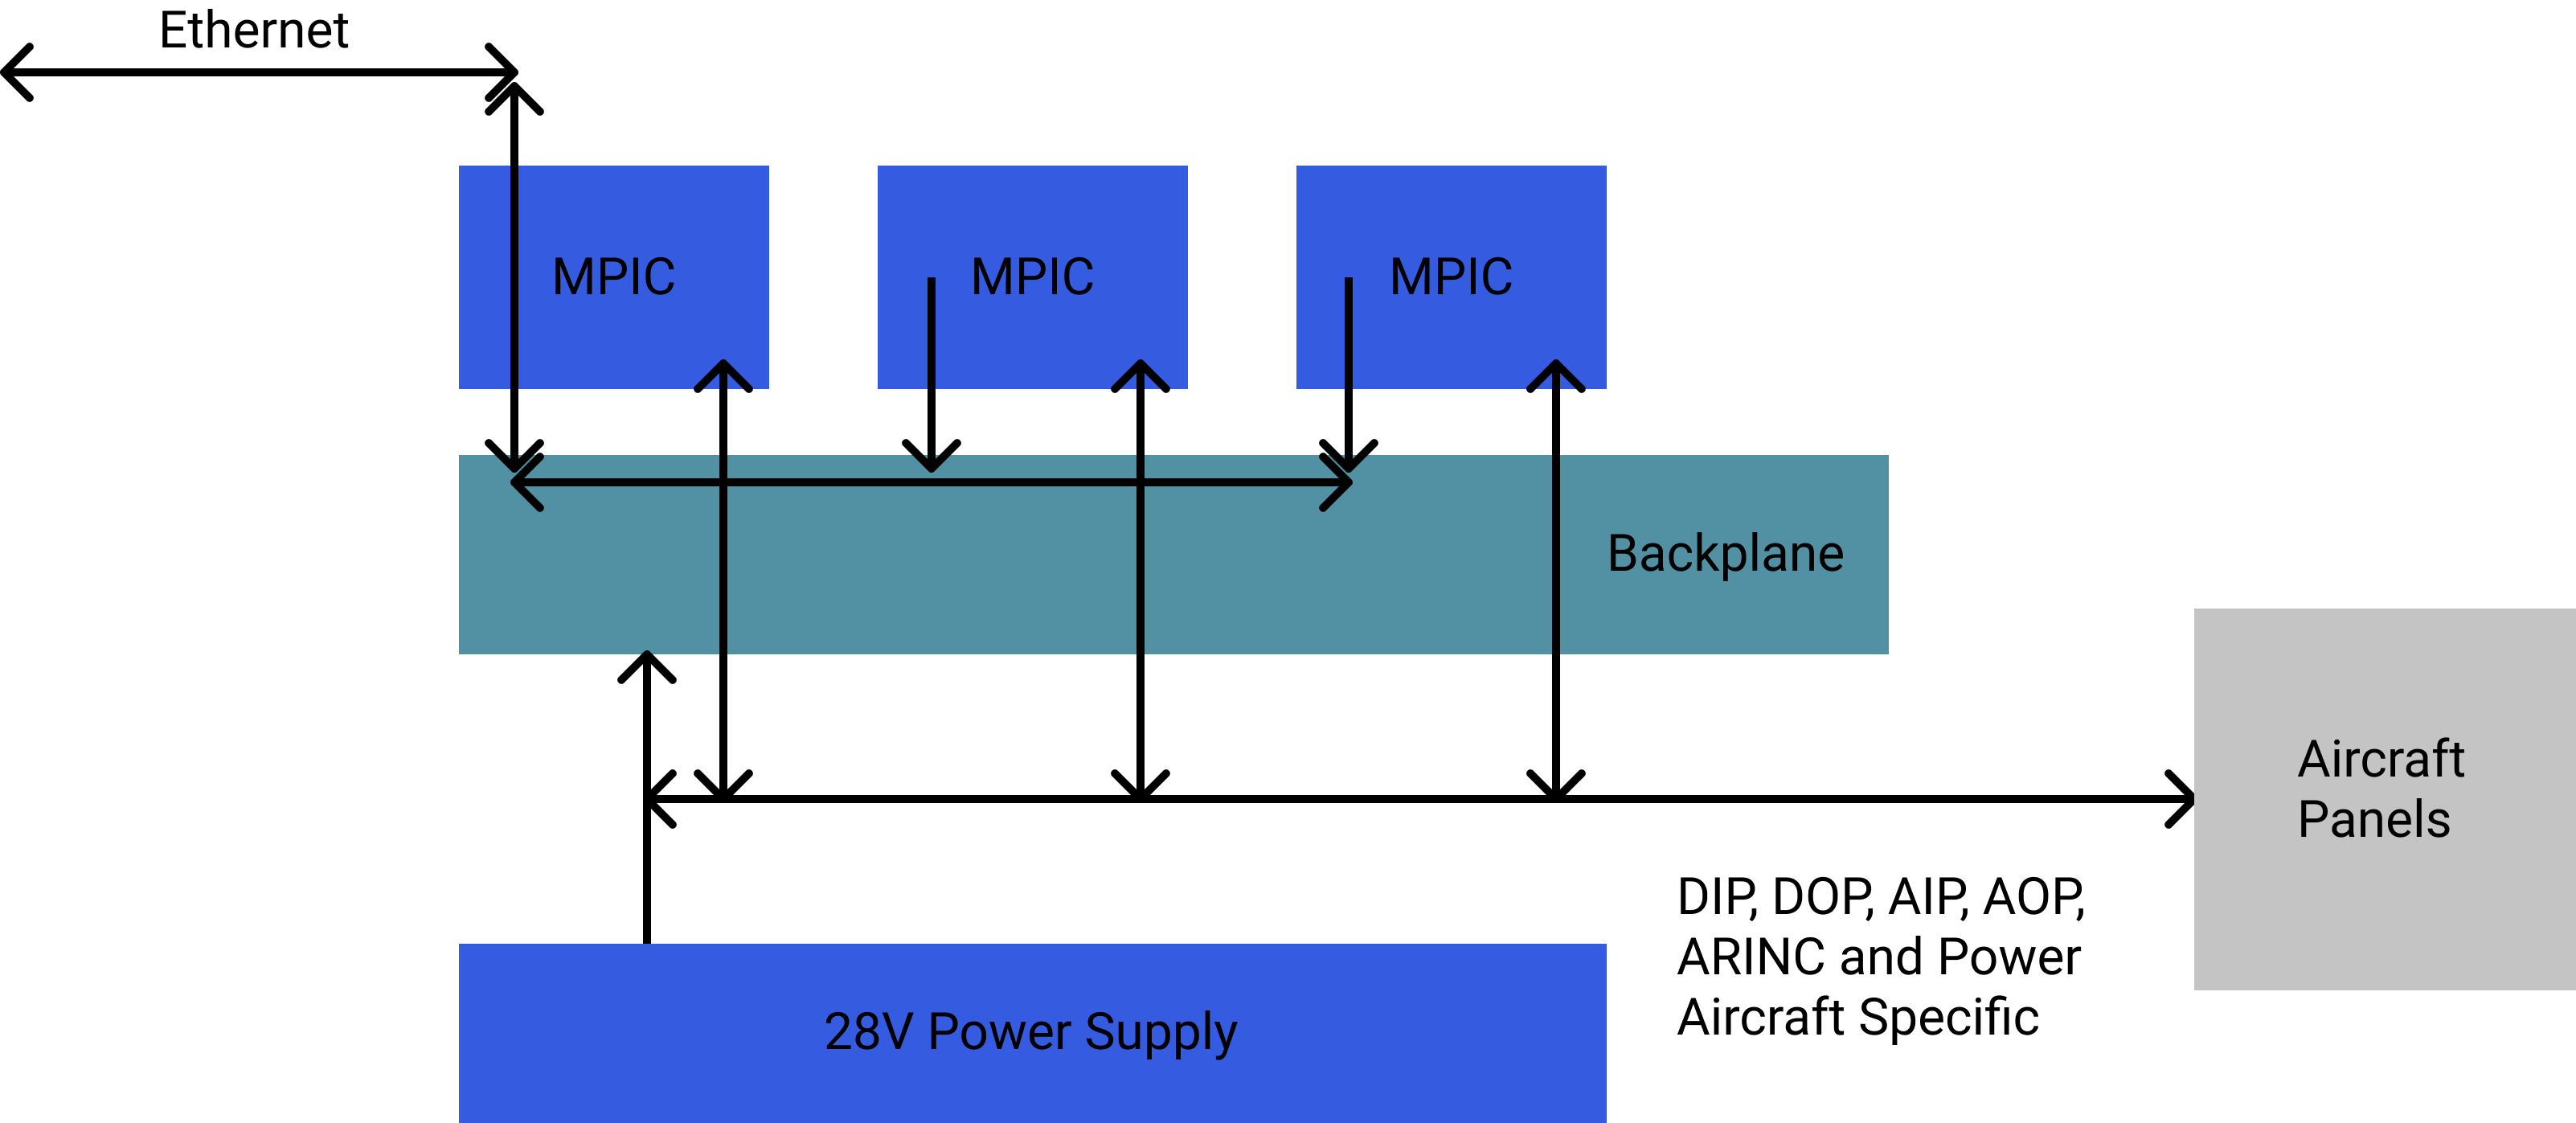
\includegraphics[width=0.6\linewidth]{img/communication path.png}
            \caption{Backplane}
        \end{figure}
    \subsection{Simulator Power Distribution}
        \begin{figure}[H]
            \centering
            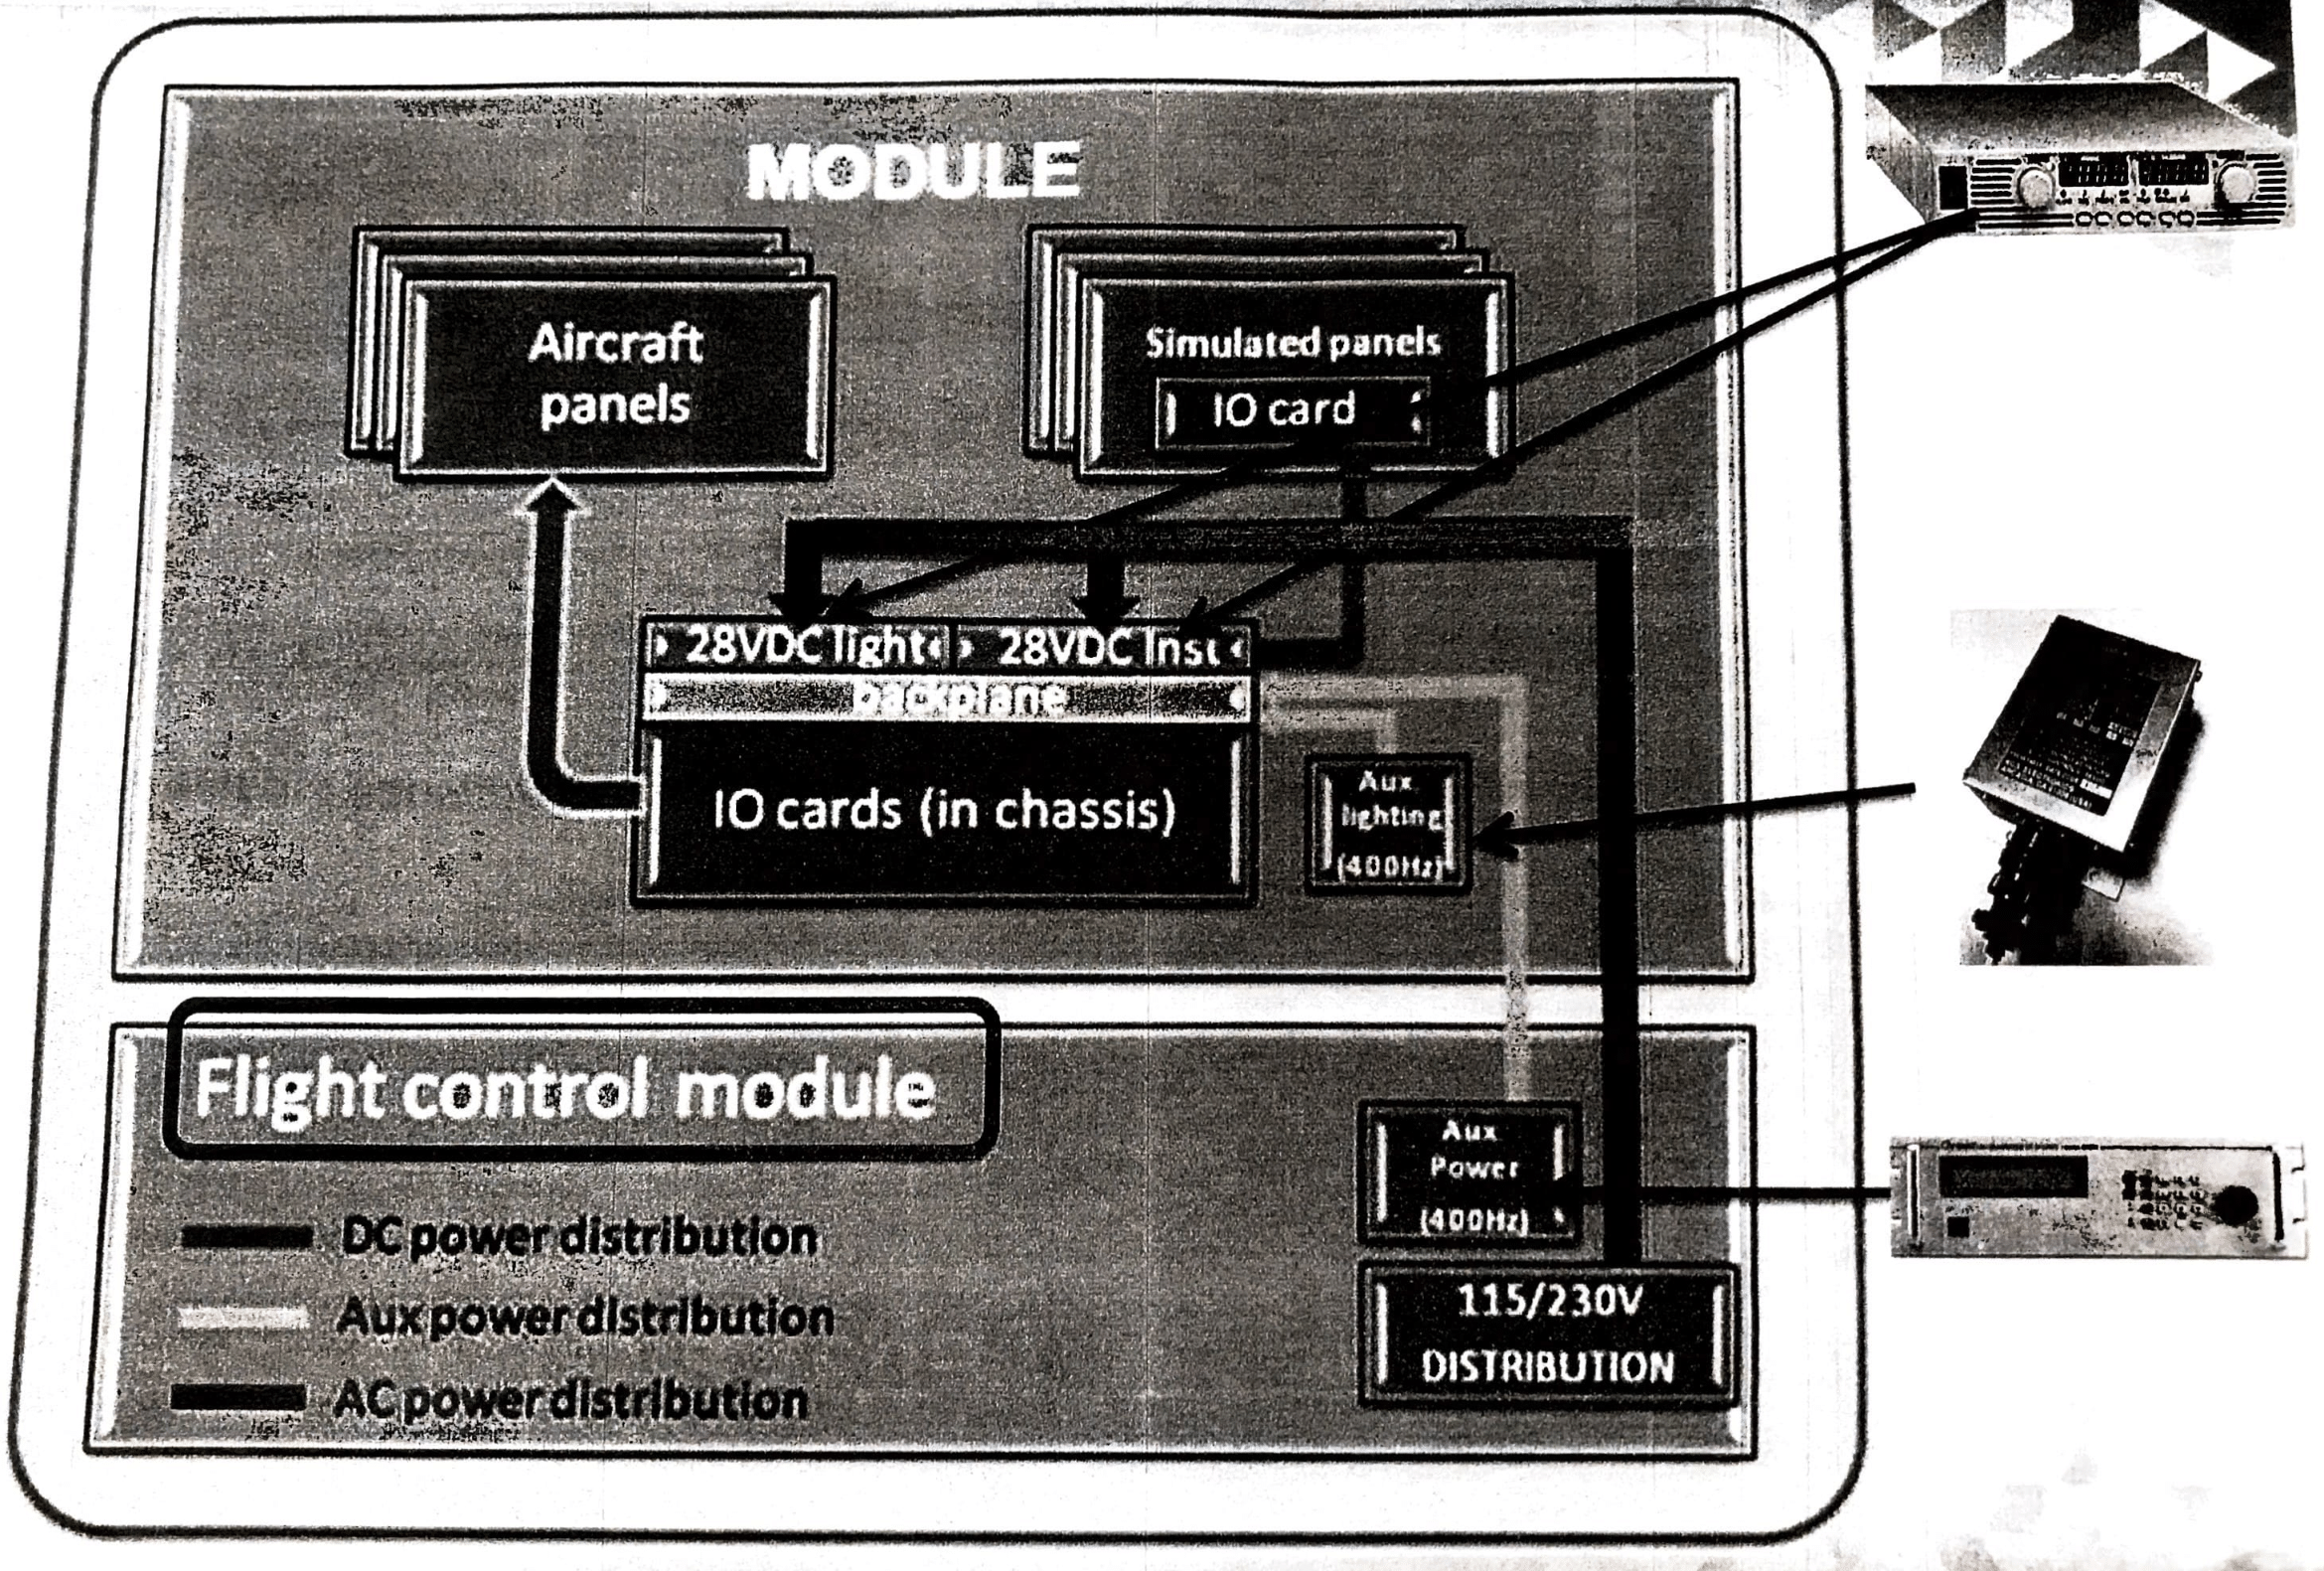
\includegraphics[width=0.6\linewidth]{img/flight-control.png}
            \caption{Flight control module}
        \end{figure}
        \begin{figure}[H]
            \centering
            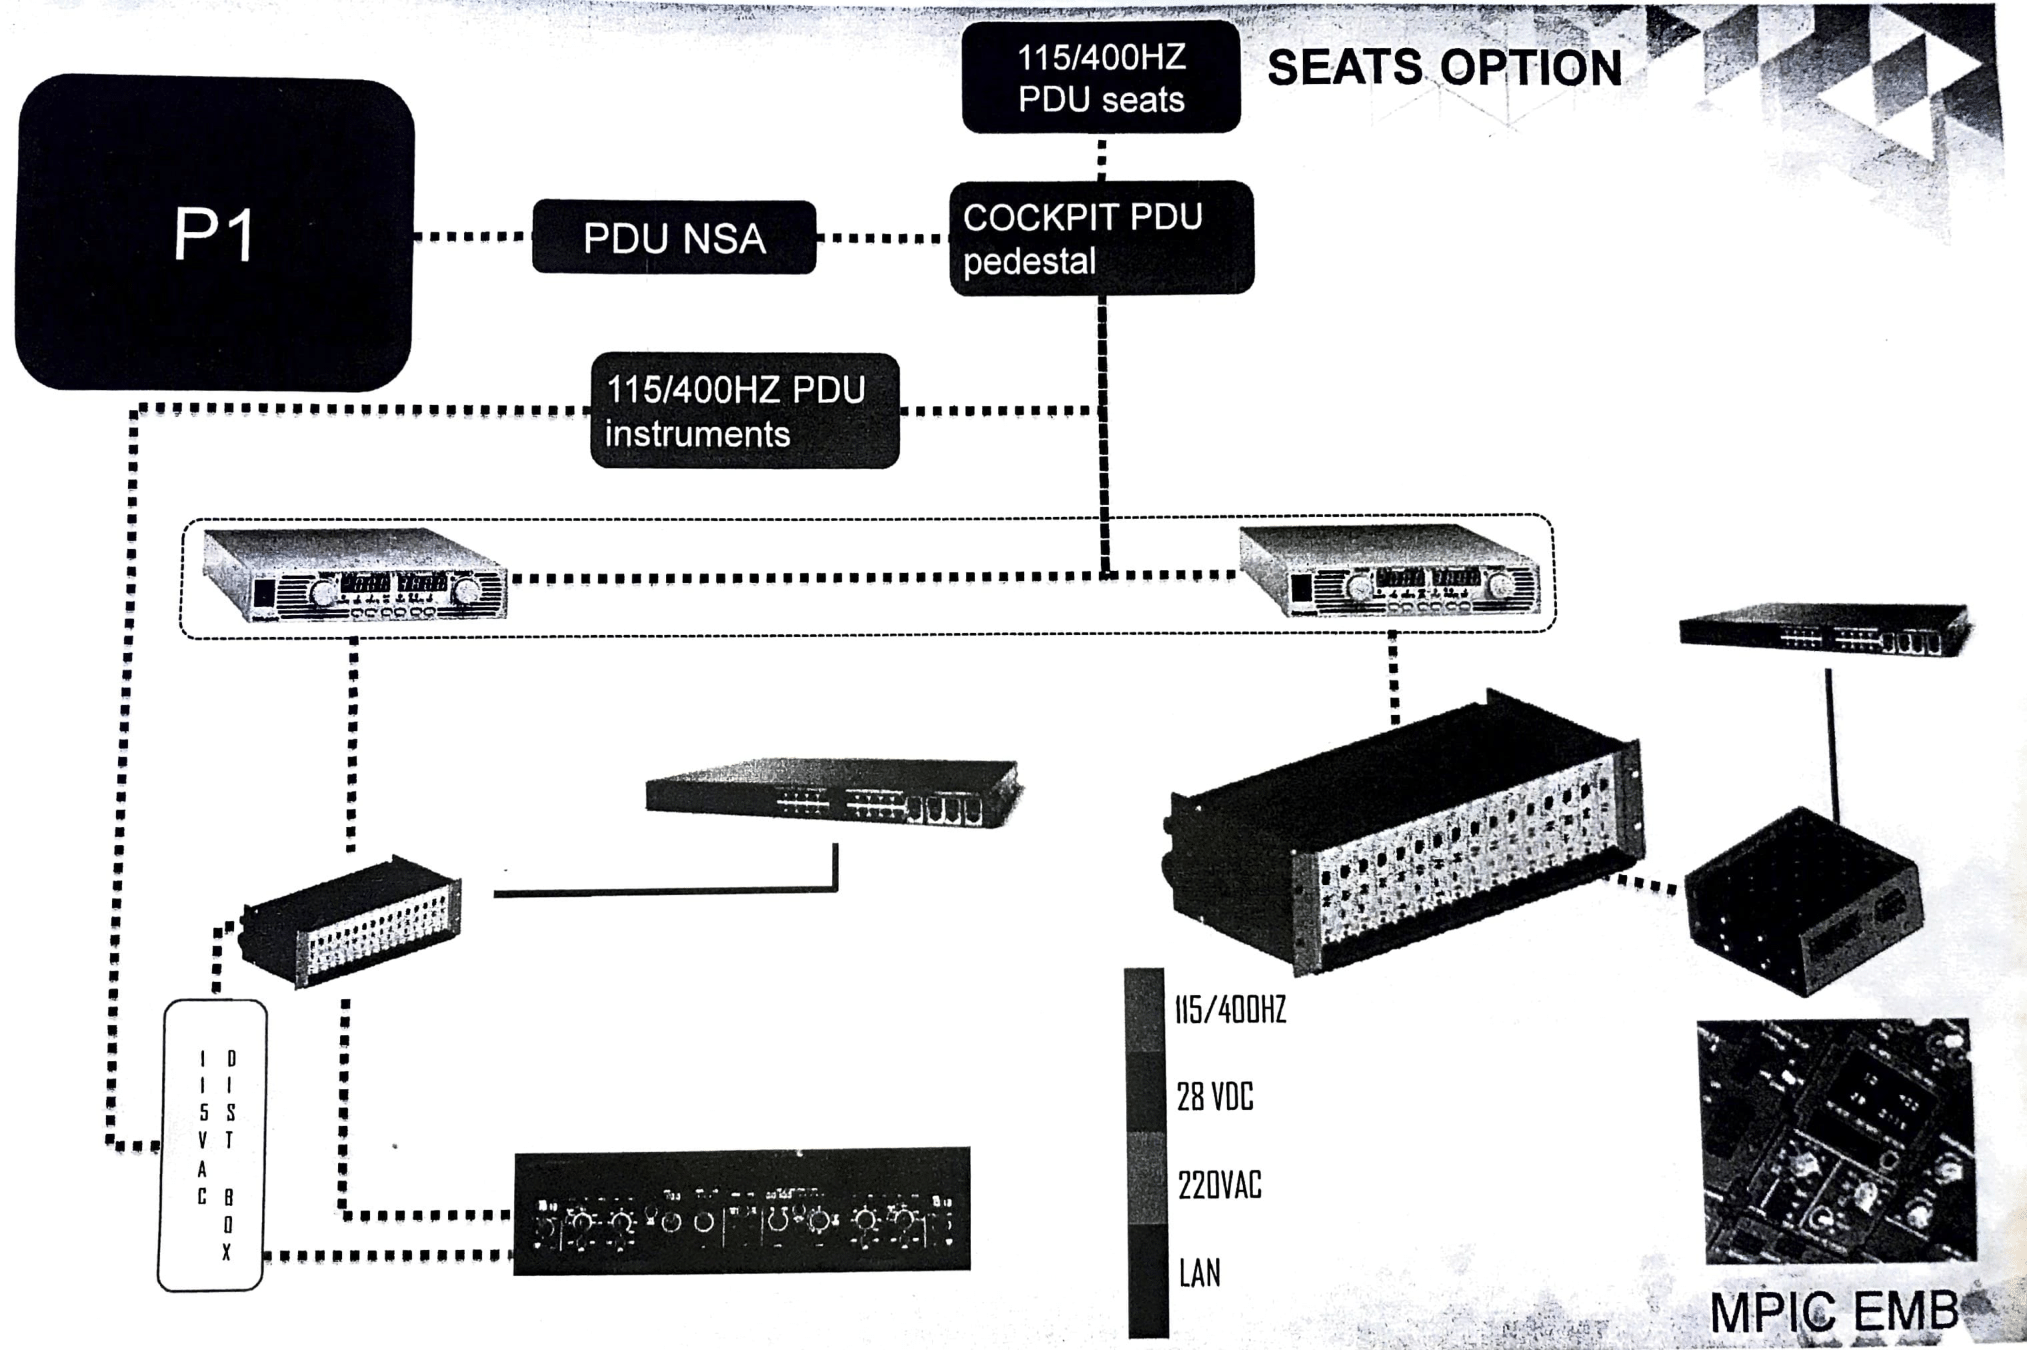
\includegraphics[width=0.6\linewidth]{img/seat-option.png}
            \caption{Seats option}
        \end{figure}
    

\section{Generic CDS Testing}
    Three generic CDSs have been initially created and tested on the CAE-MPIC. The development and tests conducted of those 
    CDSs and their related UAs helped understand the specificities of ARINC 661. Furthermore, it allowed to observe some 
    performance limitations and to determine the relevant benchmarking tests that must be further conducted. The CDSs designed 
    for the preliminary testing are very simple; the goal being the familiarization with the A661 standard.
    \subsection{PFD}
        The PFD is a non-interactive CDS. The widget positions are determined by the commands sent by the UA. The UA
        treats data received from the simulator. This new A661 PFD displays the same information as the simulator’s PFD. 
        This figure down here shows the PFD designed for the Benchmarking phase. 
        \begin{figure}[H]
            \centering
            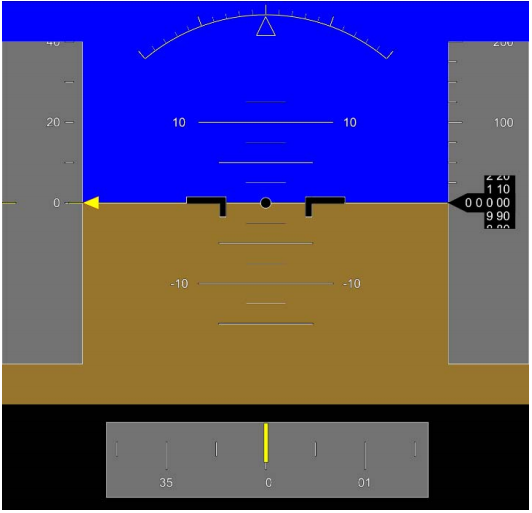
\includegraphics[width=0.6\linewidth]{img/PFD.PNG}
            \caption{Primary Flight Display (PFD)}
        \end{figure}
    \subsection{Fuel and Radio Page}
        Fuel and radio pages are interactive CDSs. Data is transmitted by the simulator to the UA that commands the appropriate W. 
        The user has the ability to send commands to the simulator. The selection is done with interactive A661\_TOGGLE\_BUTTON widgets. 
        Calculations, transmission to the simulator and display refresh are done by the UA.
        \begin{figure}[H]
            \centering
            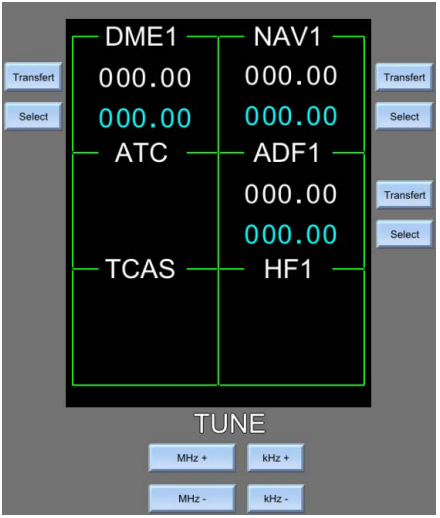
\includegraphics[width=0.6\linewidth]{img/Radio-page.PNG}
            \caption{Radio page}
        \end{figure}
        \begin{figure}[H]
            \centering
            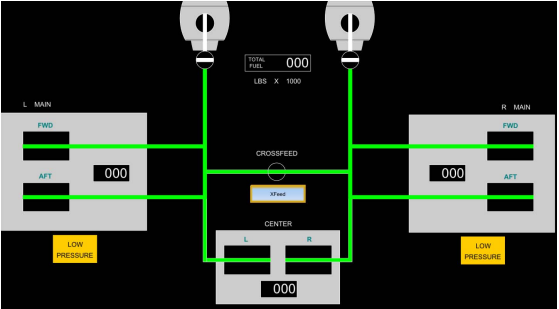
\includegraphics[width=0.6\linewidth]{img/Fuel.PNG}
            \caption{Fuel page}
        \end{figure}

    \chapter{CONCLUSION AND TOPIC ORIENTATION}

\renewcommand{\headrulewidth}{0.5pt}
\renewcommand{\footrulewidth}{0.5pt}
\thispagestyle{plain}
\pagestyle{fancy}
\fancyhf{}
\fancyhead[L]{\textbf{CHAPTER 5}}
\fancyhead[R]{\textbf{DROWSINESS DETECTION AND ALERT SYSTEM IN THE CAR}}
\raggedright
\fancyfoot[L]{From: Nguyen Van Anh Tuan}
\fancyfoot[R]{Page \thepage}

\justifying

\section{Conclusion}
    During the process of implementing this topic, I have built a system with practical applications for drivers 
    when participating in traffic, which is a sleep detection system, built on the Linux and Linux operating system. 
    Raspberry Pi 3B+ kit,with the support of OpenCV and Dlib libraries and programmed in Python programming language 
    with the task of issuing warnings when drivers doze off. \\ 
    \vspace{3mm}
    \textbf{Prodcut review:} \\ 
    To evaluate and comment objectively, I have tried to detect drowsiness in many different cases such as: front angle, 
    tilt angle, bright enough, low light, the results obtained are shown in the version below. 
    \begin{table}[ht]
        \centering
        \begin{tabular}{| l | l | l |}
            \hline
            \rowcolor{lightgray} Cases & Brightness enough & Lack of brightness \\ \hline
            Front corner & 91/100 images & 53/100 images \\ \hline
            Left tilt angle & 82/100 images & Almost undetectable \\ \hline
            Right tilt angle & 76/100 images & Almost undetectable \\ \hline
        \end{tabular}
        \caption{Results of eye state recognition in many cases}
    \end{table}
    Based on the above table, we can see that the identification results with relatively high accuracy in the case of 
    the frontal face in bright enough conditions, for the left and right tilt angles, the recognition process will be 
    more difficult. a bit, but the camera still catches the eye with high accuracy (in bright enough conditions) \\ 
    \vspace{3mm}
    On the contrary for the above three cases, the accuracy will gradually decrease in low light and almost undetectable 
    for the case of right tilt angle (low light conditions) and tilt angle greater than 40 degrees (both bright enough and low light).

\section{Limitations}
    \subsection{Advantages}
        \begin{itemize}
            \item Compact, convenient due to the small size of the Raspberry pi, it can be integrated directly on the car without 
            taking up too much space, can be integrated based on the existing security systems on the vehicle
            \item As a programmed application, it can save costs, the design and construction is also quite simple because the 
            hardware is simple, does not require complicated components
            \item Relatively high accuracy
            \item The program meets the actual requirements, the image processing time is fast, and the warning is issued in real time
        \end{itemize}
    \subsection{Disadvantages}
        \begin{itemize}
            \item Depends heavily on external conditions such as light, rotation angle,... 
            \item Face to face directly, if turning left or right with an angle greater than 40 degrees or the end of the head, 
            raising the head more than 30 degrees, it may not be detected
        \end{itemize}

\section{Development Orientation}
    \begin{itemize}
        \item Research using new, optimized and better recognition algorithms
        \item For the convenience of use, it is necessary to research and develop application software that can be controlled via smartphones
        \item Developing more diverse warning systems such as vibrating seats, or calling directly to the driver's phone, ... to wake up more effectively.
        \item When the driver shows signs of falling asleep, we can activate the car's self-driving mode and send a continuous warning to wake the driver.
    \end{itemize}

    \chapter{APPENDICES}

\renewcommand{\headrulewidth}{0.5pt}
\renewcommand{\footrulewidth}{0.5pt}
\thispagestyle{plain}
\pagestyle{fancy}
\fancyhf{}
\fancyhead[L]{\textbf{CHAPTER 6}}
\fancyhead[R]{\textbf{DROWSINESS DETECTION AND ALERT SYSTEM IN THE CAR}}
\raggedright
\fancyfoot[L]{From: Nguyen Van Anh Tuan}
\fancyfoot[R]{Page \thepage}

\justifying

\definecolor{mygray}{rgb}{0.5,0.5,0.5}

\section{Drowsiness Detection Program}

    \lstset{ 
        backgroundcolor=\color{white},   % choose the background color; you must add \usepackage{color} or \usepackage{xcolor}; should come as last argument
        basicstyle=\footnotesize,        % the size of the fonts that are used for the code
        breakatwhitespace=false,         % sets if automatic breaks should only happen at whitespace
        breaklines=true,                 % sets automatic line breakingcommentstyle=\color{mygreen},    % comment style
        captionpos=b,
        deletekeywords={...},            % if you want to delete keywords from the given language
        escapeinside={\%*}{*)},          % if you want to add LaTeX within your code
        extendedchars=true,              % lets you use non-ASCII characters; for 8-bits encodings only, does not work with UTF-8
        firstnumber=1,                % start line enumeration with line 1
        frame=single,	                   % adds a frame around the code
        keepspaces=true,                 % keeps spaces in text, useful for keeping indentation of code (possibly needs columns=flexible)
        keywordstyle=\color{blue},       % keyword style
        language=Python,                 % the language of the code
        morekeywords={*,...},            % if you want to add more keywords to the set
        numbers=left,                    % where to put the line-numbers; possible values are (none, left, right)
        numbersep=5pt,                   % how far the line-numbers are from the code
        numberstyle=\tiny\color{mygray}, % the style that is used for the line-numbers
        rulecolor=\color{black},         % if not set, the frame-color may be changed on line-breaks within not-black text (e.g. comments (green here))
        showspaces=false,                % show spaces everywhere adding particular underscores; it overrides 'showstringspaces'
        showstringspaces=false,          % underline spaces within strings only
        showtabs=false,                  % show tabs within strings adding particular underscores
        stepnumber=1,                    % the step between two line-numbers. If it's 1, each line will be numberedstringstyle=\color{mymauve},     % string literal style
        tabsize=2,	                   % sets default tabsize to 2 spaces
        title=\lstname                   % show the filename of files included with \lstinputlisting; also try caption instead of title
    }

    \begin{lstlisting}[caption={Import library}]
        from imutils.video import VideoStream
        from imutils import face_utils
        import numpy as np
        import argparse
        import imutils
        import playsound
        import time
        from threading import Thread
        import dlib
        import os
        import cv2
    \end{lstlisting}

    \begin{lstlisting}[caption={Setup sound file and turn it on}]
        wav_path = "/Drowsiness/alarm.wav"
        def play_sound(path):
            os.system('play' + path)
    \end{lstlisting}

    \begin{lstlisting}[caption={Compute the distance between 2 point A and B}]
        def e_dist(pA, pB):
            return np.linalg.norm(pA - pB)
        def eye_ratio(eye):
            #Khoang cach theo chieu doc mi tren va mi duoi
            d_V1 = e_dist(eye[1], eye[5])
            d_V2 = e_dist(eye[2], eye[4])
        
            #Khoang cach theo chieu ngang giua 2 mat
            d_H = e_dist(eye[0], eye[3])
        
            #Ty le giua chieu doc va ngang
            eye_ratio_val = (d_V1 + d_V2) / (2.0 * d_H)
            
            return eye_ratio_val
    \end{lstlisting}

    \begin{lstlisting}[caption={Define threshold level. If smaller than this is drowsiness}]
        eye_ratio_threshold = 0.25
    \end{lstlisting}

    \begin{lstlisting}[caption={Threshold so frame lien tuc nham mat}]
        max_sleep_frames = 16
    \end{lstlisting}

    \begin{lstlisting}[caption={Dem so frame ngu}]
        sleep_frames = 0
    \end{lstlisting}

    \begin{lstlisting}[caption={Check xem da canh bao hay chua}]
        alarmed = False 
    \end{lstlisting}

    \begin{lstlisting}[caption={Khoi tao cac module detect mat va facial landmark}]
        face_detect = cv2.CascadeClassifier("haarcascade_frontalface_default.xml")
        landmark_detect = dlib.shape_predictor("shape_predictor_68_face_landmarks.dat")
    \end{lstlisting}

    \begin{lstlisting}[caption={Lay danh sach cac cum diem landmark cho 2 mat}]
        (left_eye_start, left_eye_end) = face_utils.FACIAL_LANDMARKS_IDXS["left_eye"]
        (right_eye_start, right_eye_end) = face_utils.FACIAL_LANDMARKS_IDXS["right_eye"]
    \end{lstlisting}

    \begin{lstlisting}[caption={Doc tu camera}]
        vs = VideoStream(src=0).start()
        time.sleep(1.0)

        while True:

            # Doc tu camera
            frame = vs.read()

            # Resize de tang toc do xu ly
            frame = imutils.resize(frame, width=450)

            # Chuyen ve gray
            gray = cv2.cvtColor(frame, cv2.COLOR_BGR2GRAY)

            # Detect cac mat trong anh
            faces = face_detect.detectMultiScale(gray, scaleFactor=1.1,	minNeighbors=5, minSize=(100, 100),	flags=cv2.CASCADE_SCALE_IMAGE)

            # Duyet qua cac mat
            for (x, y, w, h) in faces:

                # Tao mot hinh chu nhat quanh khuon mat
                rect = dlib.rectangle(int(x), int(y), int(x + w),
                    int(y + h))

                # Nhan dien cac diem landmark
                landmark = landmark_detect(gray, rect)
                landmark = face_utils.shape_to_np(landmark)

                # Tinh toan ty le mat phai va trai va trung binh cong 2 ratio
                leftEye = landmark[left_eye_start:left_eye_end]
                rightEye = landmark[right_eye_start:right_eye_end]

                left_eye_ratio = eye_ratio(leftEye)
                right_eye_ratio = eye_ratio(rightEye)

                eye_avg_ratio = (left_eye_ratio + right_eye_ratio) / 2.0

                # Ve duong bao quanh mat
                left_eye_bound = cv2.convexHull(leftEye)
                right_eye_bound = cv2.convexHull(rightEye)
                cv2.drawContours(frame, [left_eye_bound], -1, (0, 255, 0), 1)
                cv2.drawContours(frame, [right_eye_bound], -1, (0, 255, 0), 1)

                # Check xem mat co nham khong
                if eye_avg_ratio < eye_ratio_threshold:
                    sleep_frames += 1
                    # if the eyes were closed for a sufficient number of
                    # frames, then sound the alarm
                    if sleep_frames >= max_sleep_frames:

                        if not alarmed:
                            alarmed = True
                            # Duong dan den file wav


                            # Tien hanh phat am thanh trong 1 luong rieng
                            t = Thread(target=play_sound,
                                        args=(wav_path,))
                            t.deamon = True
                            t.start()

                        # Ve dong chu canh bao
                        cv2.putText(frame, "DROWSINESS ALERT", (10, 30), cv2.FONT_HERSHEY_SIMPLEX, 0.7, (0, 0, 255), 2)

                # Neu khong nham mat thi
                else:

                    # Reset lai cac tham so
                    sleep_frames = 0
                    alarmed = False

                    # Hien thi gia tri eye ratio trung binh
                    cv2.putText(frame, "EYE AVG RATIO: {:.3f}".format(eye_avg_ratio), (10, 30),	cv2.FONT_HERSHEY_SIMPLEX, 0.7, (255, 0, 0), 2)

            # Hien thi len man hinh
            cv2.imshow("Camera", frame)

            # Bam Esc de thoat
            key = cv2.waitKey(1) & 0xFF
            if key == 27:
                break
    \end{lstlisting}

    \begin{lstlisting}[caption={End program}]
        cv2.destroyAllWindows()
        vs.stop()
    \end{lstlisting}

\section{Install Raspbian OS for Raspberry Pi 3B+}
    Require equipment for installation: 
    \begin{itemize}
        \item Micro SDHC card 32GB + adapter 
        \item Laptop for installation 
        \item Monitor 
        \item LAN cable for convenient remote control by laptop
        \item Power 5v, 2.5A (at least 1A) 
    \end{itemize}
    \subsection{Step 1}
        Download Raspbian OS ISO file to laptop and extract it
        \begin{figure}[H]
            \centering
            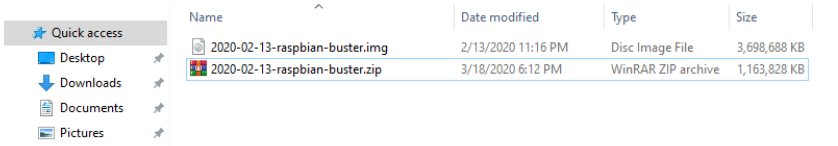
\includegraphics[width=0.8\linewidth]{img/download.PNG}
            \caption{The file contain Raspbian OS}
        \end{figure}
    \subsection{Step 2}
        Install SD card formater and win32 Disk Imager software
    \subsection{Step 3}
        Insert MicroSD card into card reader in laptop and check drive name of disk assigned to memory card to avoid 
        confusion causing other data loss. 
    \subsection{Step 4}
        Run SD Card Formater software to format memory card then run Win32 Disk Imager start install OS to the memory card
        \begin{figure}[H]
            \centering
            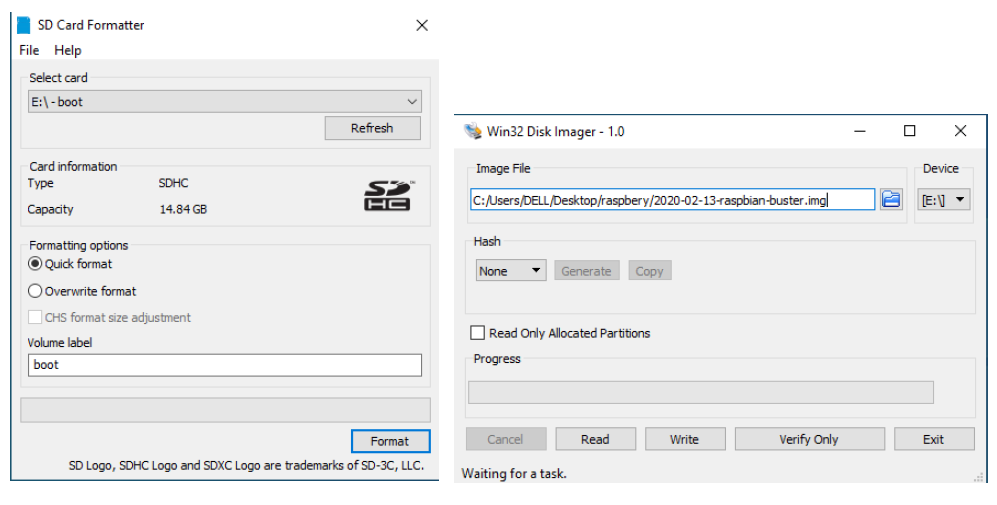
\includegraphics[width=0.8\linewidth]{img/format-disk.PNG}
            \caption{Format disk and install OS into memory card}
        \end{figure}
\section{Install Necessary Libraries}
    \subsection{OpenCV}
        \textbf{\$sudo apt install python3-pip} \\ 
        \vspace{3mm}
        This step allow us to install pip in Python 3. Next we using Pip command to install OpenCV library by using: \\ 
        \vspace{3mm}
        \textbf{\$sudo pip3 install opencv-python} \\ 
        \vspace{3mm}
        Next we install another package to run the code: 
        \begin{itemize}
            \item imutils
            \item numpy
            \item playsound 
            \item dlib
        \end{itemize}
\section{Run program}
    At last, we run this command to run program with 2 components is sound file and data file of HaarCascade front face: \\
    \vspace{3mm}
    \textbf{\$python3 main.py}
    \begin{figure}[H]
        \centering
        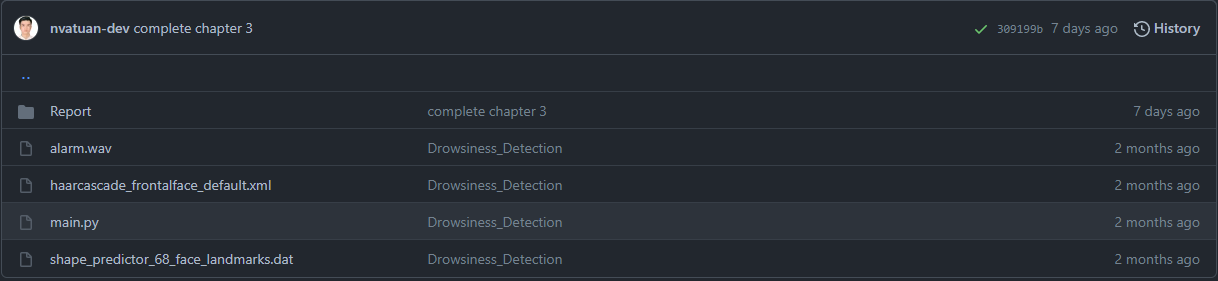
\includegraphics[width=0.8\linewidth]{img/folder-tree.PNG}
        \caption{Folder tree of project}
    \end{figure}

    \newpage
    \thispagestyle{plain}
    \begin{center}
        \Huge{\textbf{THE REFERENCES}}
    \end{center}
    \vspace{3mm}
    \begin{enumerate}
        \item Adrian Rosebrock, May 8th 2017, "\textit{Drowsiness detection with OpenCV}"
        \item Nguyen Chien Thang, February 26th 2017, "\textit{Computer Vision \& Pi – Lap dat Pi tren xe hoi de phat hien tai xe ngu gat}"
        \item Raspberry Pi, January 28th 2019, "\textit{Raspberry Pi Compute Module 3+}"
        \item Hai Ha, February 20th 2019, "\textit{Histogram of Oriented Gradients}"
        \item Adrian Rosebrock, April 3rd 2017, "\textit{Facial landmarks with dlib, OpenCV, and Python}"
        \item Adrian Rosebrock, April 24th 2017, "\textit{Eye blink detection with OpenCV, Python, and dlib}"
        \item Wikipeidia, April 13th 2021, "\textit{Euclidean distance}"
        \item OpenCV, May 29th 2021, "\textit{Cascade Classifier}"
    \end{enumerate}

\end{document}